
\documentclass[12pt]{article}
\usepackage[english]{babel}
\usepackage{inputenc}
\usepackage{amsmath}
\usepackage{graphicx}
\usepackage[version=4]{mhchem}
\usepackage{mathtools}

\usepackage[margin=0.8in]{geometry}

\title{Combustion Processes in Thermochemical Propulsion}

\date{}
\author{Notes by Riccardo Canola}

\begin{document}

\maketitle

\newpage

\tableofcontents

\newpage

\section{Phenomenological introduction to combustion processes}

Combustion is the development of chemical reactions of oxido-reduction, strongly exothermic and very fast, due to heat and catalyst products accumulation.
\begin{itemize}
    \item \textit{Diffusion flame}: the reactants diffuse into each other during the chemical reaction.
    \item \textit{Premixed flame}: the reactants are perfectly mixed before chemical reaction.
\end{itemize}

\begin{figure}[!ht]
\centering
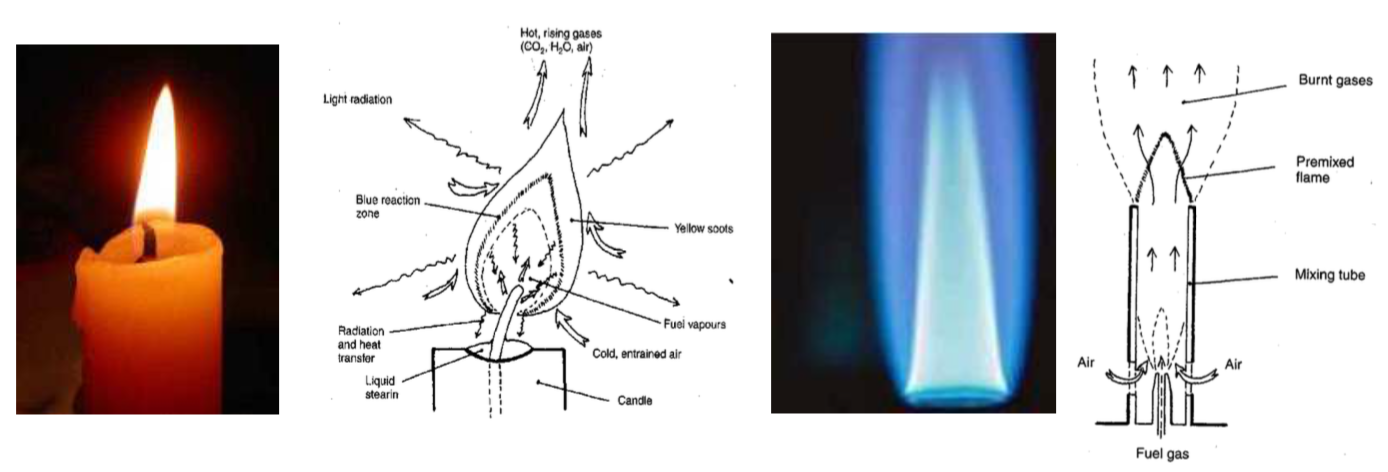
\includegraphics[width=0.8\textwidth]{figures/diffusion_premixed.png}
\end{figure}

\subsection{Industrial burners}

\begin{itemize}
    \item \textit{gas burners}: a swirler is responsible for high turbulence which increases flame speed propagation.
    \item \textit{liquid fuel burners}: the fuel is injected in form of spray. In order to anchor the flame, the air jet is introduced with a swirl motion, which causes a pressure drop and recirculation zone close to the central axis of the burner. The flame is longer and the soot is responsible for the higher radiation.
\end{itemize}

\subsection{Internal combustion engines}

\begin{itemize}
    \item \textit{Otto}: the combustion process in this kinf of engine which is spark-ignited, develop through a premixed flame with a laminar or turbulent flame propagation.
    \item  \textit{Diesel}: the combustion process develops through a diffusion flame and the flame speed propagation is turbulent.
\end{itemize}

\subsection{Ramjets}

Can be used above $Mach 2$. The gas velocity at the entrance of the combustion chamber is much faster than the flame propagation speed. The recirculation zone grants a permanence of the gas for several milliseconds. Temperature at turbine's blades has to be below a certain value.

\subsection{Rockets}

\begin{itemize}
    \item \textit{Liquid rocket}: they provide a good performance and permit re-ignition. The injector design is the most delicate aspect for the engine performance.
    \item \textit{Solid rocket}: fuel is a solid cylinder provided with a central perforation which forms the combustion chamber. The thrust is proportional to the combustion surface, therefore it is designed in a way that the combustion follows a rule ($r_{b}=ap^{n}$). The solid fuel (alluminum powder) contains the oxidizer and therefore the flame should be premixed. However, oxidizer decomposition products can react in diffusion flame. The interaction between premixed and diffusion flames is the most critical part of any modeling approach.

\begin{figure}[!ht]
\centering
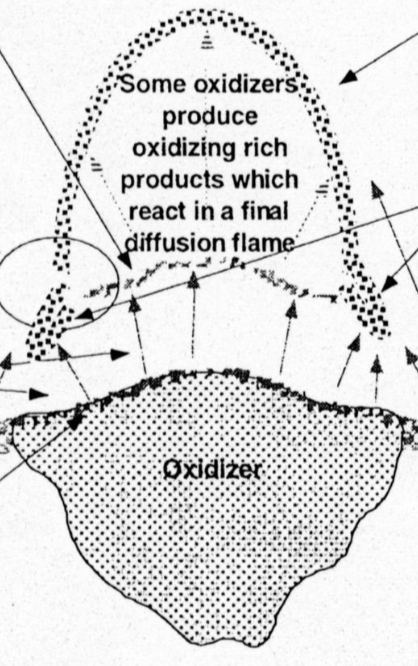
\includegraphics[width=0.3\textwidth]{figures/flame_solid.png}
\end{figure}

    \item \textit{Hybrid rocket}: fuel solid and oxidizer liquid. Oxidizer are introduced in form of spray. The flame develops inside the boundary layer ($r_{b}=aG_{ox}^{n}$).

\begin{figure}[!ht]
\centering
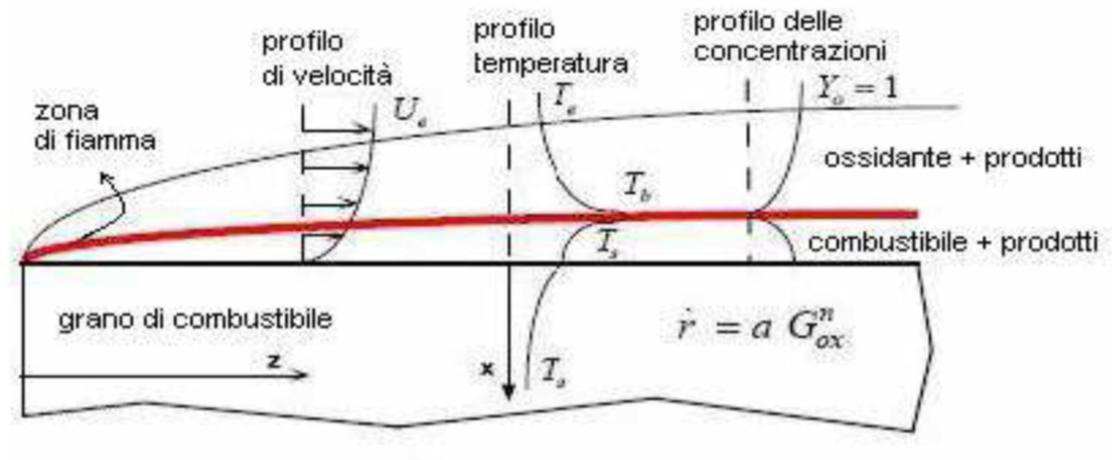
\includegraphics[width=0.8\textwidth]{figures/hybrid.png}
\end{figure}

\end{itemize}

\subsection{Flames}

Flame is a discontinuity surface separating reactants from combustion products. Its peculiar property is the capability of self-sustaining and propagation.

\begin{itemize}
    \item homogeneous and heterogeneous
    \item laminar and turbulent
    \item premixed and diffusion
    \item deflagration and detonation
\end{itemize}

\begin{figure}[!ht]
\centering
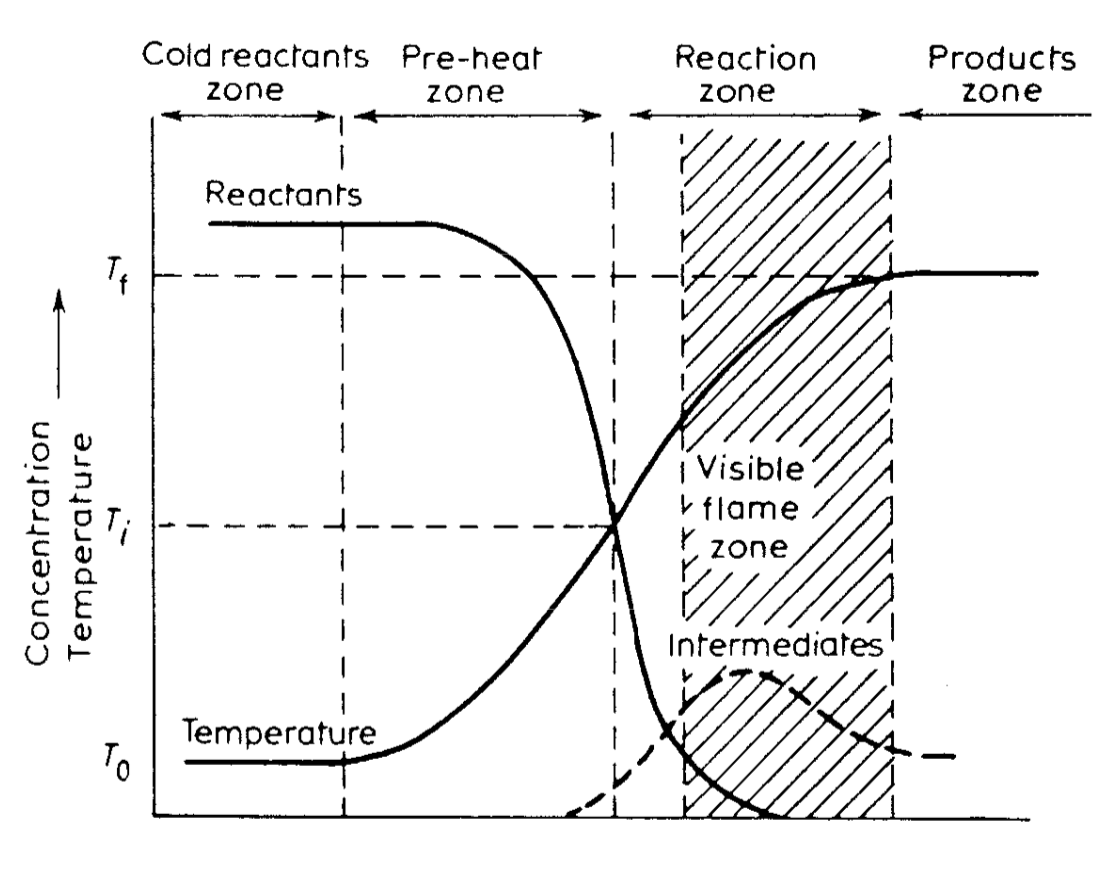
\includegraphics[width=0.5\textwidth]{figures/premixed_structure.png}
\caption{Premixed flame structure}
\end{figure}

\begin{figure}[!ht]
\centering
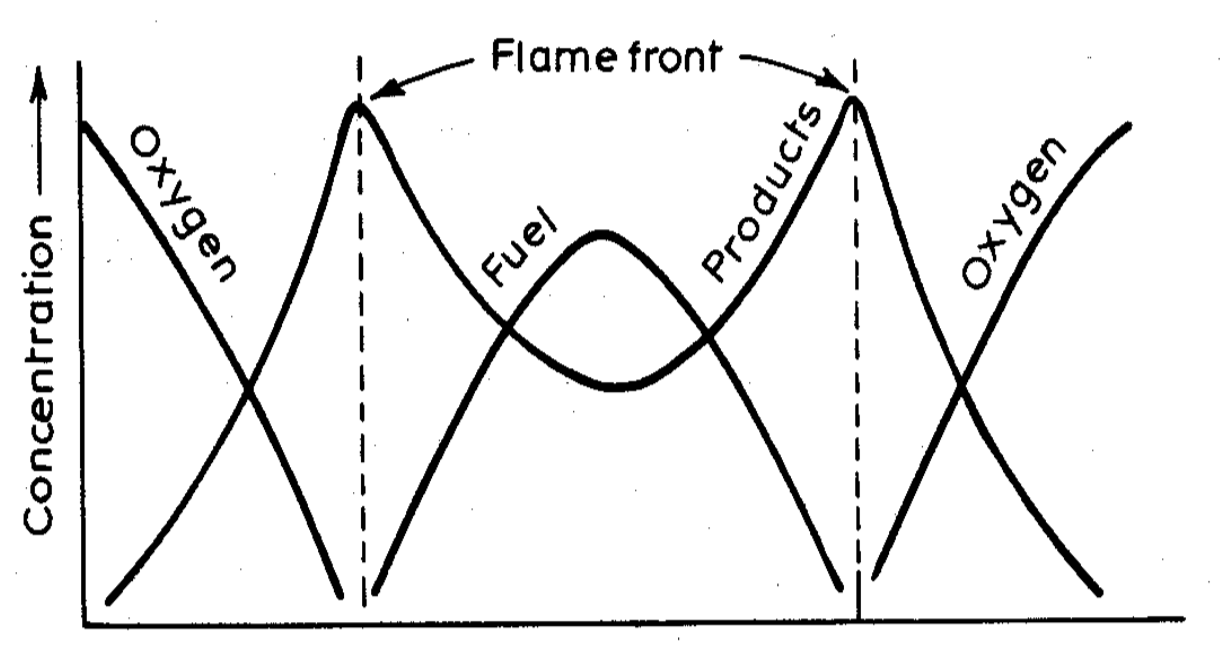
\includegraphics[width=0.5\textwidth]{figures/diffusion_structure.png}
\caption{Diffusion flame structure}
\end{figure}

\subsection{Flame propagation rate}

It is the speed relative to the fresh mixture. It is a constant for a specific mixture and it is proportional to the amount of mixture that in the time unit can be changed into combustion products.

\begin{itemize}
    \item methane/air: $0.4 m/s$
    \item methane/oxygen: $4.0 m/s$
    \item hydrogen/air: $1.8 m/s$
    \item hydrogen/oxygen: $10 m/s$
\end{itemize}

\subsection{Abiabatic flame temperature}

It is the temperature of combustion products in an adiabatic system. It depends on the fuel and oxidizer nature and on the mixture ratio.

\subsection{Mixture composition}

\begin{itemize}
    \item \textit{Mixture ratio} $\alpha$: amount of oxidizer, in mass or volume, linked to the fuel mass or volume unit.
    \item \textit{Equivalence ratio} $\phi$: mixture ratio normalized with respect to the stoichiometric ratio:
    \begin{equation}
        \phi = \frac{(Ox/F)}{(Ox/F)}_{stech}
    \end{equation}
    \item \textit{Air excess}: E.A.$=\phi-1$
\end{itemize}

\subsection{Inflammability limits}

Minimum volumetric concentration of fuel in the mixture (\textit{lower inflammability limit}) and maximum volumetric concentration of fuel in the mixture (\textit{upper inflammability limit}) in order to ignite the mixture. A mixture can be ignited only if the mixture ratio is within well defined limits.

\subsection{Reaction heat}

Energy released in the stoichiometric reaction of the fuel within molecular gaseous oxygen.

\subsection{Flash point}

Flash point of a liquid fuel is the lowest temperature at which, an amount of fuel vapour is produced which is able to be ignited by a suitable ignition device. The value decreases when pressure decreases and the oxygen content increases. The temperature of self-ignition is usually much higher than the temperature of the flash point. The two temperatures have a completely different physical meaning.

\newpage

\section{Fundamentals of chemical thermodynamics}

Thermochemistry provide a quantitative assessment of the energy released in a chemical reaction.
For a generic chemical equilibrium the mathematical formalism proposed by Penner is considered:

\begin{equation}
    \sum_{j=1}^{N} v_{i}^{'}M_{i} \rightarrow  \sum_{j=1}^{N} v_{i}^{''}M_{i}
\end{equation}

\begin{itemize}
    \item $M$ is the generic chemical substance
    \item $v^{'}$ are the stoichiometric coefficients relative to the reactants
    \item $v^{''}$ are the stoichiometric coefficients relative to the products
    \item $N$ is the total number of chemical components of the mixture

\end{itemize}

\subsection{Standard formation enthalpy $\Delta h_{f}^{0}$}

The standard enthalpy of formation $\Delta h_{f}^{0}$ of a substance at a given temperature is defined as the enthalpy of the substance obtained at the standard thermodynamic state.
\begin{itemize}
    \item The standard thermodynamic state of a given substance is the ideal gas or liquid or solid state that the substance assumes at the conditions of $p=1$ atm and temperature T.
\end{itemize}
The standard enthalpy of formation is a state property, therefore we are only interested in the initial and final state.

\subsection{Reaction enthalpy $\Delta h_{r}$}

The reaction enthalpy $(\Delta h_{r})_{T}$ at a given temperature T, is defined as the thermal energy released or absorbed during the reaction:
\begin{equation}
    \sum_{j=1}^{N} v_{i}^{'}M_{i} \rightarrow  \sum_{j=1}^{N} v_{i}^{''}M_{i} + \Delta h_{r}
\end{equation}
If the final temperature of the products is the same of the temperature of the reactants, the energy balance does not include contributions linked to the change of temperature:
\begin{equation}
    \Delta H_{r}=(\Delta h)_{T}^{0}= \sum_{products} v_{j}^{''}(\Delta h_{f}^{0})_{T} -\sum_{reactants} v_{j}^{'}(\Delta h_{f}^{0})_{T}
\end{equation}
This equation states that if the standard enthalpy of formation is known, the reaction enthalpy of any reaction can be evaluated.
\\
The energy released or absorbed has a definite value determined by the initial and final state:
\begin{itemize}
    \item for a reaction at constant pressure: $Q=\Delta H$
    \item for a reaction at constant volume: $Q=\Delta U$
\end{itemize}
the enthalpy totally involved, is given by:
\begin{equation}
    \Delta h_{r}= \sum_{products} v_{j}^{''}[\Delta (h_{f}^{0})_{T_{0}}+(h_{T_{2}}-h_{T_{0}})] -\sum_{reactants} v_{j}^{'}[\Delta (h_{f}^{0})_{T_{0}}+(h_{T_{1}}-h_{T_{0}})]
\end{equation}

\subsection{Reaction advancement}

The reaction advancement, defined as "$z$", is a molar concentration change. It is $z=0$ at the beginning of the reaction, and $z=1$ at the end. Consequently, the reaction enthalpy becomes $z\Delta u$ for a constant volume or $z\Delta h$ for a constant pressure.

\subsection{Fundamental thermochemical laws}

\begin{itemize}
    \item \textbf{Lavoisier and Laplace}: the energy associated to a chemical reaction in one direction is equal and opposite in sign, to the energy associated to the same reaction in the inverse direction.
    \item \textbf{Hess}: the energy associated to a chemical reaction at constant pressure or constant volume, is the same if the reaction is developed in one or more steps. It does not depend on the path, consequently, reactions can be treated as algebraic equations.
\end{itemize}

\subsection{Bond energies}

Bond energy is the energy required to break a bond between two atoms. Usually, this energy depends on the distance between atoms. It is necessary to consider the resonance in the molecule, which gives higher values of the standard formatioon enthalpy (it happens in the benzene $C_{6}H_{6}$).

\subsection{Adiabatic flame temperature}

The equation for the computation of the entalpy of reaction is:
\begin{equation}
    \Delta h_{r}= \sum_{products} v_{j}^{''}[\Delta (h_{f}^{0})_{T_{0}}+(h_{T_{2}}-h_{T_{0}})] -\sum_{reactants} v_{j}^{'}[\Delta (h_{f}^{0})_{T_{0}}+(h_{T_{1}}-h_{T_{0}})]
\end{equation}
if the heat released is used to heat the products, the products temperature $T_{2}$ is defined as \textit{adiabatic flame temperature}, therefore $(\Delta h_{r})=0$ and the equation becomes:
\begin{equation}
    \sum_{products} v_{j}^{''}[\Delta (h_{f}^{0})_{T_{0}}+(h_{T_{2}}-h_{T_{0}})] =\sum_{reactants} v_{j}^{'}[\Delta (h_{f}^{0})_{T_{0}}+(h_{T_{1}}-h_{T_{0}})]
\end{equation}
if the products are known, it is possible to obtain the flame temperature.
\\
The heat released to the combustion products under adiabatic conditions is:
\begin{equation}
    -\Delta H_{r} = N_{tot}C_{P}\Delta T_{adiabatic}
\end{equation}
\begin{equation}
    \Delta T_{adiabatic} = \frac{\Delta H_{r}}{C_{P}N_{tot}}
\end{equation}
 For high temperature \textit{dissociation reactions} (strongly endothermic) develop. They produce other species ($CO, H_{2},...$), decreasing the global exothermicity of the reaction and the adiabatic flame temperature.
\begin{figure}[!ht]
\centering
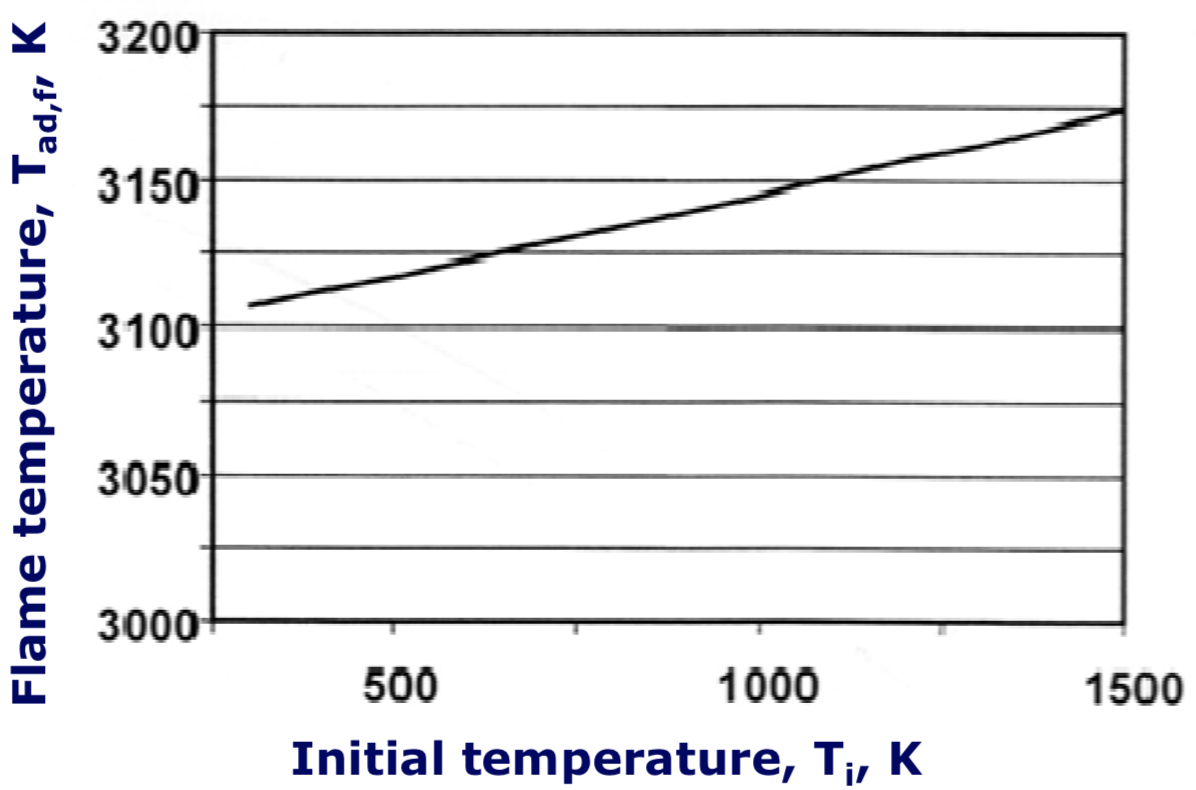
\includegraphics[width=0.5\textwidth]{figures/dissociation.png}
\end{figure}
Trend of the adiabatic flame temperature, significant increases of $T_{i}$ cause modesr increases of $T_{ad}$ due to dissociation reactions.

\subsection{Equilibrium ($K_{p}$)}

Chemical equilibrium is one of the most important concepts in thermochemical propulsion. It assumes that at the exit from the combustion chamber, chemical phenomena behave as quasi-steady (much faster) with respect to the fluid dynamic phenomena:
\begin{equation}
    \frac{t_{ch}^{*}}{t_{fl}^{*}} << 1
\end{equation}
A system is in a stable equilibrium when its state can be changed reversibly by an infinitesimmal amount. Such system obeys to the relationship:
\begin{equation}
    TdS=de+pdV=dh-Vdp
\end{equation}
combustion processes are characterized by constant pressure and temperature, therefore the condition can be rewritten as:
\begin{equation}
    d(e+pV-TS)_{p,T}=d(h-TS)_{p,T}=0
\end{equation}
where the \textit{Gibbs free energy}, is:
\begin{equation}
    F=(e+pV-TS)=h-TS
\end{equation}
Thus, the stable equilibrium condition of any chemical system working at constant temperature and pressure, is:
\begin{equation}
    (dF)_{p,T}=0
\end{equation}
It is possible to show that the criterium of stable equilibrium to small perturbations leads to:
\begin{equation}
    \Delta F^{0}(T)=-RTlnK_{p} = \sum_{j=1}^{N}(v_{j}^{''}-v_{j}^{'})F_{j}^{0}
\end{equation}
\begin{equation}
    K_{p}(T)= \frac{\prod_{j=1}^{N}(p_{j})^{v_{j}^{''}}}{\prod_{j=1}^{N}(p_{j})^{v_{j}^{'}}}
\end{equation}
$K_{p}$ is the \textit{equilibrium constant} and $p_{j}$ are the partial pressure of the mixture.

\subsection{The physical meaning of $K_{p}$}

The more negative $\Delta F^{0}$ is, the larger is $K_{p}$. This means that the reaction is more spontaneous. When the free energy of the reactants and products is the same, the reaction has no tendency to proceed in either direction.
The practical importance of $K_{p}$ is that it is independent on total pressure and can be a unique function of the temperature.
\begin{equation}
    \Delta F^{0}(T)=-RTlnK_{p}
\end{equation}
Since the variation $\Delta F^{0}$ depends only on temperature also the second member depends only on temperature.
Consequently, for a given mixture it is possible to tabulate $K_{p}(T)$. This is an extremely interesting result for propulsion applications since the free energy change at the standard pressure $p=1 atm$ determines the equilibrium conditions at all other pressure.
\begin{equation}
    \Delta F_{p,T}=0
\end{equation}
is the equilibrium condition (not $\Delta F^{0}$!)

\subsection{Equilibrium constants}

\begin{itemize}
    \item $K_{p}=\prod_{j=1}^{N}(p_{j})^{{v_{j}^{''}}-{v_{j}^{'}}} \rightarrow$ partial pressure
    \item $K_{n}=\prod_{j=1}^{N}(n_{j})^{{v_{j}^{''}}-{v_{j}^{'}}} \rightarrow$ number of partial moles
    \item $K_{X}=\prod_{j=1}^{N}(X_{j})^{{v_{j}^{''}}-{v_{j}^{'}}} \rightarrow$ partial molar function
    \item $K_{c}=\prod_{j=1}^{N}(M_{j})^{{v_{j}^{''}}-{v_{j}^{'}}} \rightarrow$ partial molar concentration
    \item $K_{Y}=\prod_{j=1}^{N}(Y_{j})^{{v_{j}^{''}}-{v_{j}^{'}}} \rightarrow$ partial mass fraction
\end{itemize}
but only $K_{p}$ and $K_{c}$ are functions of just one variable and don't depend on pressure. Propulsion applications preferably uses $K_{p}$.

\subsection{Mixture composition and flame temperature}

The problem of thermochemical equilibrium in combustion chambers requires to know simultaneously temperature and composition of the mixture (mass and energy conservation equations).\\
We can decouple the problem.

\subsubsection{Flame temperature}

We suppose the combustion chamber as an open thermodynamic system, where chemical reactions occur at constant pressure And we suppose known the composition of the reactive mixture before and after the reactions.

\begin{equation}
    \sum_{j=1}^{N}n_{j}^{'}\{(\Delta h_{f}^{0})_{T_{ref}}+[\Delta h^{0}]_{T_{ref}}^{T_{j}}\}_{j} \rightarrow
    combustor
    \rightarrow
    \sum_{j=1}^{N}n_{j}^{''}\{(\Delta h_{f}^{0})_{T_{ref}}+[\Delta h^{0}]_{T_{ref}}^{T_{c}}\}_{j}
\end{equation}

$T_{j}$ is the temperature of injection of $n_{j}$ moles of reactants in the combustion chamber, and $T_{c}$ is the common temperature of exit from the combustion chamber of the $n_{j}$ moles of products.
$T_{ref}$ is the reference table of the available tables.\\
The energy conservation requires:

\begin{equation}
    \sum_{j=1}^{N}n_{j}^{'}[(\Delta h_{f}^{0})_{T_{ref}}+(h_{T_{j}}^{0}-h_{T_{ref}}^{0})]_{j}
    =
    \sum_{j=1}^{N}n_{j}^{''}[(\Delta h_{f}^{0})_{T_{ref}}+(h_{T_{c}}^{0}-h_{T_{ref}}^{0})]_{j}+\Delta h_{ext}
\end{equation}

where $h_{T}^{0}-h_{T_{ref}}^{0} = \int_{T_{ref}}^{T} Cp_{j}(T)dT$ are tabulated values of the molar thermal enthalpy.\\
The temperature $T_{C}$ resulting from the conservation energy equation is called \textit{flame temperature}. It increases if enthalpy lost to the environment decreases. If $\Delta h_{ext}=0$, the adiabatic flame temperature is the maximum admissible temperature in the combustion chamber.

\subsubsection{Available and absorbed enthalpy}

\begin{equation}
    \Delta h_{available}^{0} = \left\{
    \sum_{j=1}^{N}n_{j}^{'}[(\Delta h_{f}^{0})_{T_{ref}}+(h_{T_{j}}^{0}-h_{T_{ref}}^{0})]_{j}
    -
    \sum_{j=1}^{N}n_{j}^{''}[(\Delta h_{f}^{0})_{T_{ref}}]_{j}\right\} - \Delta h_{ext}
\end{equation}

is the enthalpy available due to chemical reactions, while:

\begin{equation}
    \Delta h_{absorbed}^{0} = \sum_{j=1}^{N}n_{j}^{''}(h_{T_{c}}^{0}-h_{T_{ref}}^{0})_{j}
\end{equation}

is the enthalpy absorbed to warm up the combustion products.

\begin{figure}[!ht]
\centering
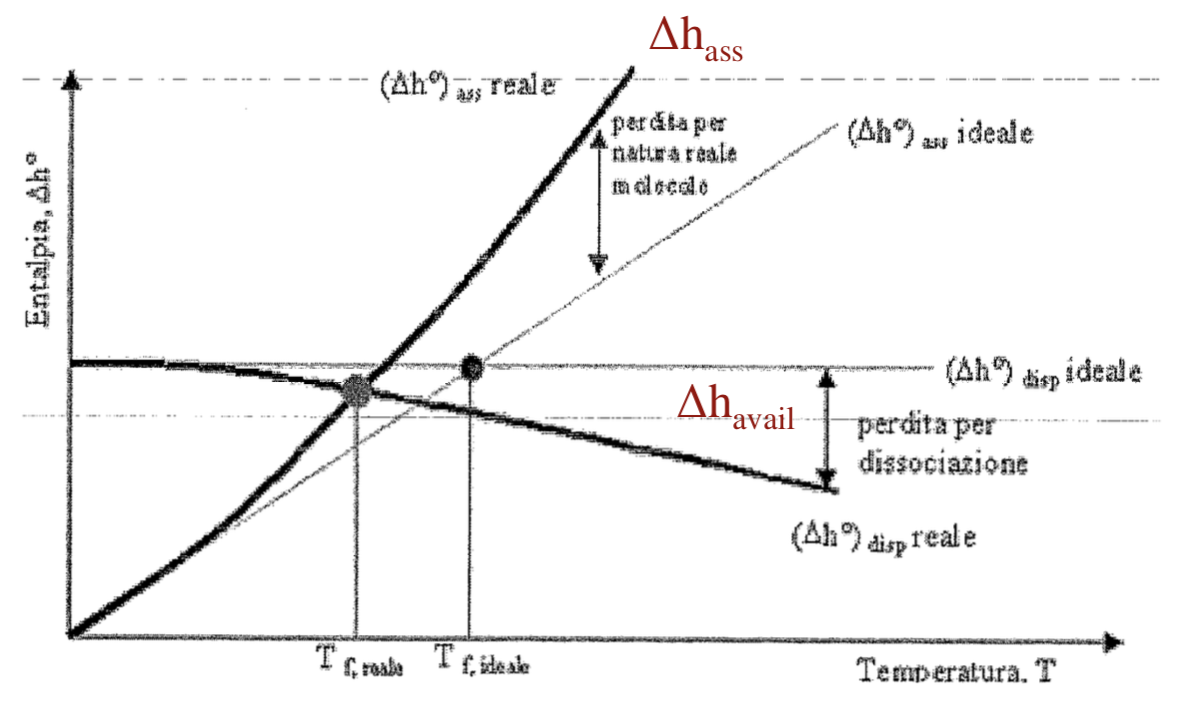
\includegraphics[width=0.6\textwidth]{figures/availablevsabsorbed.png}
\end{figure}

Increasing combustion temperature implies a fall in the available enthalpy due to molecular dissociation and the simultaneous growth of the absorbed enthalpy.\\
These phenomena, show a limit of operations for all thermal propulsion system which is approximately at $5000 K$.

\subsubsection{Mixture composition}

In this case it is knownn the working pressure $p_{c}$, $T_{j}$, $T_{c}$.

\begin{equation}
    n_{j}^{'} \rightarrow n_{j}^{''}?
\end{equation}

\newpage

\section{Fundamentals of chemical kinetics in combustion processes}

\begin{itemize}
    \item Chemical thermodynamics involves systems containing a high number of chemical species. The considered chemical quantity is the \textit{mole}.
    \item Chemical kinetics focuses on systems in which singular species are involved. The considered chemical quantity is the \textit{molecule}.
\end{itemize}

The study of the thermodynamic aspects of combustion only require the global reaction. However, when mechanisms involved in the reaction process are many, they cannot occur in one step of reaction. The singular step is named \textit{elementary reaction} and the set of elementary reactions is the so called \textit{reaction mechanism}.\\
In this section we study the rate of change at which elementary reactions develop, and the governing laws of the reaction rate.\\
Then the important concept of \textit{chain of reactions} is introduced.\\
Chemical reactions can be divided, looking at the reaction rate, into:
\begin{itemize}
    \item reactions of \textit{explosive nature}
    \item reactions of non-explosive nature
\end{itemize}
The explosive nature (high reaction rate) characterizes the combustion systems, but reactions non-explosive are also important (production of pollutants).

\subsection{Chemical reaction rate}

The reaction rate \textbf{$\dot{\omega}$} [$\frac{mole}{cm^{3}s}$] depends on:
\begin{itemize}
    \item concentration of reactants
    \item temperature (T)
    \item pressure (p)
    \item presence of catalysts or reaction inhibitors
    \item radiant effects
\end{itemize}
and can be expresses as the concentration rate decresase of one reactant, or concentration rate increase of a produced species.\\
Consider the elementary reaction in a closed system:
\begin{equation}
    aA+bB+... \rightarrow cC+dD+...
\end{equation}
now, let's define \textit{z} the reaction development:
\begin{equation}
    -\frac{dn_{A}}{a}dt =
    -\frac{dn_{B}}{b}dt =
    +\frac{dn_{C}}{c}dt =
    \frac{dz}{dt}
\end{equation}
and the reaction rate can be defines as:
\begin{equation}
    \dot{\omega} = \frac{dz}{dt}
\end{equation}
and does not depend on the chemical species considered.

\subsection{Law of mass action}

The chemical reaction is given by:
\begin{equation}
    \dot{\omega} = k \prod_{i=1}^{N}[M_{i}]^{v_{i}}
\end{equation}
where $K$ is the \textit{rate constant} which depend only on temperature T given by Arrhenius Law.

\subsection{Molecular collision theory}

Essential requirement for the occuring of an elementary reaction is that species come in contact. The reaction rate cannot be higher than the \textit{collision frequency} between A and B, named \textbf{$Z_{AB}$} which for gasses is given by the gas kinetic theory.\\
Real rate is $10^{10}$ times lower of the collision frequency $Z_{AB}$. Also, collision have to be considered effective only if their energy is higher than a \textit{treshold value} \textit{$E_{a}$}.

\subsection{The activated complex theory}

\begin{equation}
    X+YZ \rightarrow XY+Z
\end{equation}
$d_{YZ}$ is the distance between Y and Z and $d_{XY}$ is the distance between X and Y. The curves of the picture are curves at equal potential energy. Stability is given by two valleys. For the initial system point a and for the final system point b.
The transition from the intial system to the final system requires the moving from the first valley to the second, following the path which is the most efficient from the energetic point of view, crossing c (\textit{punto di sella}). The crossing of the point c can occur if the system receives a suitable amount of energy (molecular vibrations) that is given by an exponential term ($E_{a}/RT$) which explains the concepts of efficient collision which leads to the \textit{activated complex}.

\begin{figure}[!ht]
\centering
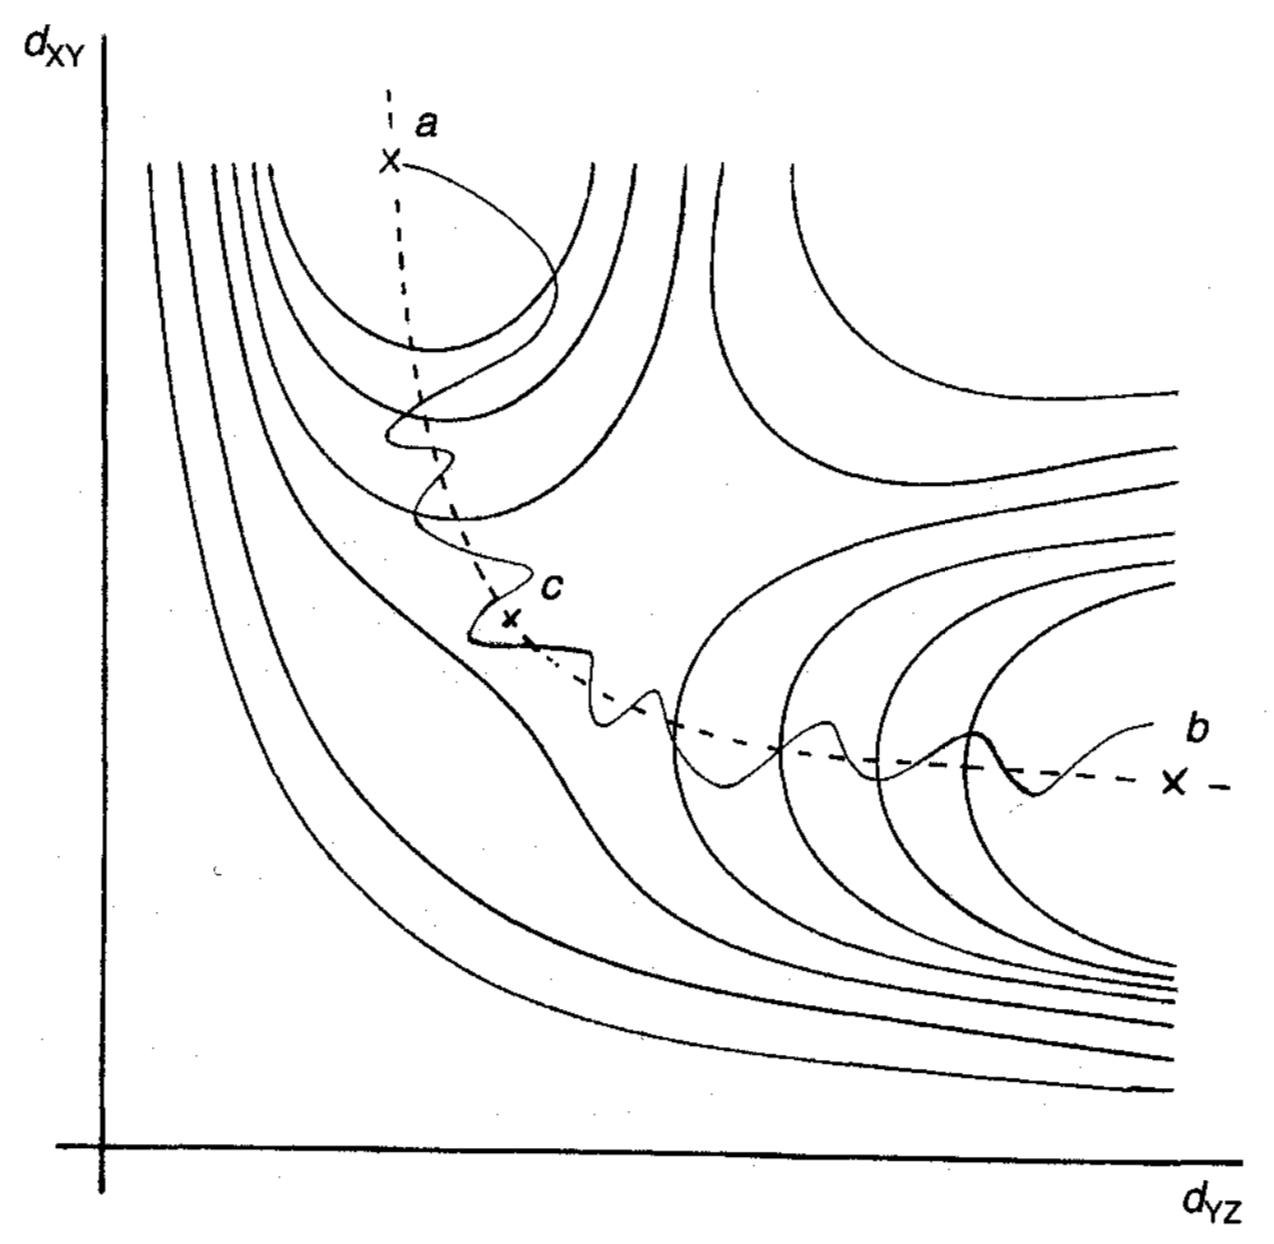
\includegraphics[width=0.35\textwidth]{figures/pointc.png}
\end{figure}



\subsection{Arrhenius law}

\begin{figure}[!htb]
    \centering
    \begin{minipage}{.5\textwidth}
        \centering
        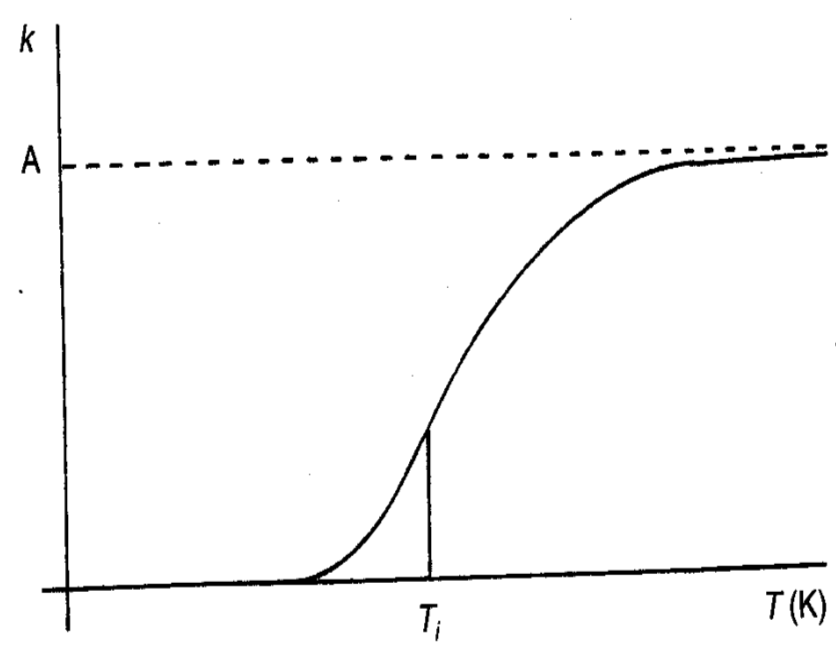
\includegraphics[width=0.8\linewidth, height=0.15\textheight]{figures/arr1.png}
    \end{minipage}%
    \begin{minipage}{0.5\textwidth}
        \centering
        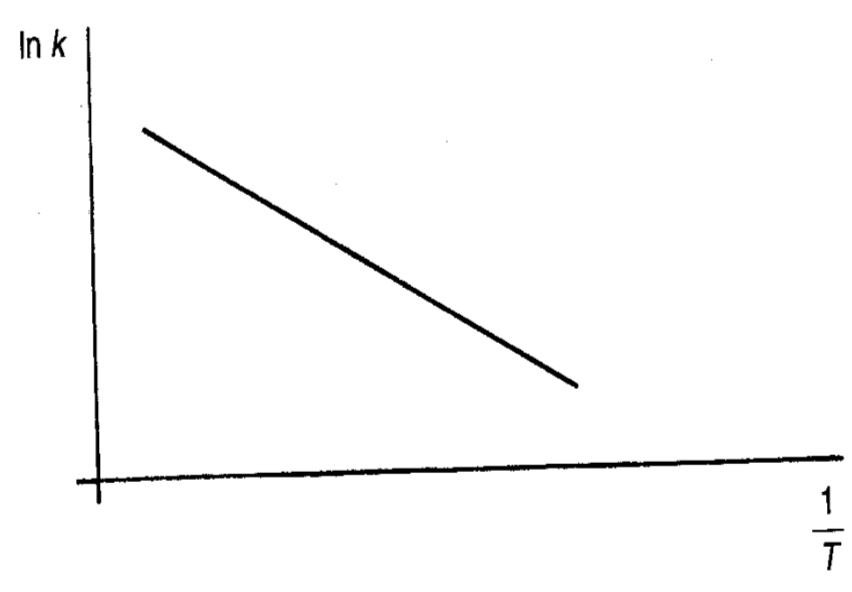
\includegraphics[width=0.8\linewidth, height=0.15\textheight]{figures/arr2.png}
    \end{minipage}
\end{figure}

Trend of the rate constant vs temperature according to the Arrhenius Law ($lnK=g(1/T)$). $K$ tends to the frequency factor when the temperature becomes very high. Reactions kinetics are investigated significantly below this limit.

\begin{equation}
    K=BT^{a}e^{-E_{a}/RT}
\end{equation}
where $BT^{a}$ is the collision frequency and $e^{-E_{a}/RT}$ is the Boltzmann factor (the fraction of collisions which have an energy larger than the activation energy $E_{a}$).\\
Thus, for a second order reaction:
\begin{equation}
    B+C \rightarrow products
\end{equation}
the reaction is given by:
\begin{equation}
    \frac{d[B]}{dt} = - K[B][C] = -A[B][C]e^{-E_{a}/RT}
\end{equation}
where $A=BT^{a}$.
Given a chemical reaction, the specific reaction rate does not depend on concentrations $[M]_{i}$, it depends only on temperature.

\subsection{Activation energy}

A collision leads to the formation of a transient chemical species, an aggregate which is defined activated complex $X^{+}$. The energy between two atoms of a diatomic molecul ($A_{2}$) depends on the distance between the two atoms. When an atom B becomes closer to the molecul, the distance between the atoms A and A changes. The collision of B with $A_{2}$ leads to the formation of the activated complex $BA_{2}^{+}$ , which has a much higher reactivity than that of neutral atoms.\\
The reaction follows the reaction path with the lowest energy among all possible paths.

\begin{itemize}
    \item the activation energy for direct and indirect reactions is not the same
    \item the direct and reverse reactions have different rate constant
    \item $E_{a}$ is the required energy in order to develop the reaction, it is the energy to bring reactants over the energy treshold needed
\end{itemize}

\subsection{Reaction order}

The net rate of production of a chemical species is given by:
\begin{equation}
    \frac{d[M]_{i}}{dt} = (v_{i}^{''}-v_{i}^{'})\dot{\omega}=(v_{i}^{''}-v_{i}^{'})K_{f}\prod_{i=1}^{N}[M]_{i}^{v_{i}^{'}}
\end{equation}
The reaction process is of order $v_{i}^{'}$ respect to $M_{i}$, the \textit{global reaction order m} is given by:
\begin{equation}
    m = \sum_{i=1}^{N}v_{i}^{'}
\end{equation}
in other words, the sum of the exponents of the reactants concentration terms.

\subsection{One-step chemical reactions}

\subsubsection{First order reactions}

\begin{itemize}
    \item Decomposition of the molecule: $A_{2}\xrightarrow{k_{f}} 2A$
    \begin{equation}
        \frac{d[A]}{dt}=2K_{f}[A_{2}]
    \end{equation}
    \item Dissociation of the molecule:
    $AB\xrightarrow{k_{f}} A+B$
    \begin{equation}
        \frac{d[AB]}{dt}=-K_{f}[AB]
    \end{equation}
    \item Bimolecular reaction:
    $A+C\xrightarrow{k_{f}} D$ \\where $[C]>[A]$
    \begin{equation}
        \frac{d[A]}{dt}=-\frac{d[D]}{dt}=-K_{f}[A][C]=k'[A]
    \end{equation}
    $k'$ is a new specific rate constant, defined considering that $[C]=constant$.
\end{itemize}
All monomolecular reactions are of order 1, but not all the first order reactions are monomolecular.

\subsubsection{Second order reactions}

Often chemical reactions follow second order reactions. In more complex reaction, the second order means that the slow step, which is responsible for the reaction rate, is bimolecular.
\begin{equation}
 A+B\xrightarrow{k_{f}} AB
\end{equation}
    \begin{equation}
        \frac{d[AB]}{dt}=K_{f}[A][B]=-\frac{d[A]}{dt}=-\frac{d[B]}{dt}
    \end{equation}
\begin{equation}
   2A\xrightarrow{k_{f}} C+D
\end{equation}
    \begin{equation}
        2\frac{d[C]}{dt}=2\frac{d[D]}{dt}=2K_{f}[A]^{2}=-\frac{d[A]}{dt}
    \end{equation}

\subsubsection{Third order reactions}
\begin{itemize}
    \item Trimolecular reaction:
    \begin{equation}
    2NO+O_{2}\xrightarrow{k_{f}} 2NO_{2}
    \end{equation}
    \item Involvement of a third body:
    \begin{equation}
    M+2A_{2}\xrightarrow{k_{f}} A_{2}+M^{*}
    \end{equation}
    \begin{equation}
        \frac{d[A_{2}]}{dt}=k_{f}[M][A]^{2}=-\frac{1}{2}\frac{d[A]}{dt}
    \end{equation}
    \begin{equation}
        \frac{d[A]}{dt}=-2k_{f}[M][A]^{2}
    \end{equation}
\end{itemize}
If $[M]=const,  \frac{d[A]}{dt}=-k'[A]^{2}$\\ in this case the reaction order is reduced from 3 to 2.

\subsection{Consecutive Reactions}

\begin{equation}
    A+B\xrightarrow{k_{2}}AB\xrightarrow{k_{2}}C+D
\end{equation}
\begin{equation}
        \frac{d[AB]}{dt}=k_{1}[A][B]=-\frac{d[A]}{dt}=-\frac{d[B]}{dt}
\end{equation}
\begin{equation}
        \frac{d[AB]}{dt}=k_{2}[AB]=-\frac{d[C]}{dt}=-\frac{d[D]}{dt}
\end{equation}
\begin{equation}
        \frac{d[AB]}{dt}=k_{1}[A][B]-k_{2}[AB]
\end{equation}

With the development of the reaction, the concentrations of A and B decrease, and the concentrations of C and D increase.

\subsection{Competitive reactions}

\begin{equation}
    A+B\xrightarrow{k_{1}}AB
\end{equation}
\begin{equation}
    A+B\xrightarrow{k_{2}}E+F
\end{equation}

\begin{itemize}
    \item $1^{st}$ reaction:
    \begin{equation}
        \frac{d[A]}{dt}=-k_{1}[A][B]
    \end{equation}
     \item $2^{nd}$ reaction:
    \begin{equation}
        \frac{d[A]}{dt}=-k_{2}[A][B]
    \end{equation}
    \begin{equation}
        \frac{d[A]}{dt}=-(k_(1)+k_{2})[A][B]
    \end{equation}
\end{itemize}
The specific rate constant can depend on temperature. The extrapolation of the rate law, obtained in a certain temperature interval, could lead to a mistake if extrapolated to a higher temperature interval.

\subsection{Opposite reactions}

TODO

\newpage

\section{Laminar premixed and diffusion flames}

A flame, which depends on the interplay of chemical and physical processes, is caused by the self-propagating of exothermic reaction. Two properties can be defined and measured: the \textit{burning rate or flame propagation rate ($S_{i}$)} and the \textit{adiabatic flame temperture ($T_{f,ad}$)}. \\
Burning rate increases at reduced pressure and at elevated temperatures. The mixture ratio at stoichiometric conditions lead to a maximum value.\\
The flame will be held at a fixed position (stationarity) since the gas flow rate is equal in magnitude, but opposite in sign, to the burning rate.\\
The goal is to predict the value of the burning rate from knowledge of the physical and chemical properties.

\subsubsection{The Mallard - Le Chatelier Model (P)}

It is assumed:
\begin{itemize}
    \item $(T_{f}-T{i}/\delta_{r})$ is the temperature gradient where $\delta_{r}$ is the reaction zone thickness
    \item $\lambda(T_{f}-T{i}/\delta_{r})$ is the \textit{heat flux} where $\lambda$ is the thermal conductivity
    \item the heat flux must be equal to the increase of enthalpy $\dot{m}C_{p}(T_{i}-T{0})$
    \item $\dot{m}=S_{L}\rho$ is the mass flow for a one-dimensional system, where \textbf{$S_{L}$} is the \textit{flow velocity}.
\end{itemize}
Therefore:
\begin{equation}
    S_{L} = \bigg[\frac{\lambda(T_{f}-T{i})\dot{\omega}}{\rho C_{p}(T_{i}-T{0}}\bigg]^{\frac{1}{2}}
\end{equation}
As $\frac{\lambda}{\rho C_{p}} = \alpha$ is the \textit{thermal diffusity}, the approach lads to the important conclusion that:
\begin{equation}
    S_{L}\sim[\alpha \dot{\omega}]^{\frac{1}{2}}
\end{equation}

which is not an accurate calculation of the burning rate (flame propagation rate), but enables to take into account parameters to be then predicted with some precision.

\subsubsection{Propagation by active species (P)}

The Mallard - Le Chatelier model assumes that the flame propagation is due entirely to heat conduction. A new model propose that the diffusion of active species ahead of the flame could provide an other explanation (\textit{thermal vs diffusional theories}).\\
A theory based purely on diffusion assumes isothermal propagation and that the equilibrium is attained at the end of the reaction zone. Then, the \textit{active centers} diffuse upstream into the reaction zone where their concentrations are in excess of equilibrium values for the given temperature.\\
A concentration profile can be found by solving the diffusion equation and the following burning rate is obtained:

\begin{equation}
    S_{L}^{2} =\frac{\sum_{j}K_{j}[F]X_{j}D_{j0}}{X^{'}}
\end{equation}
\begin{itemize}
    \item $K_{j}$ is the specific rate for the reaction of the j-th species
    \item $X_{j}$ is the mole fraction of species j in the combustion products
    \item $[F]$ is the fuel concentration
    \item $D_{j0}$ is the diffusion coefficient of species j
    \item $X^{'}$ is the mole fraction of the combustion product
\end{itemize}

However, due to powerful computers available, it is no longer necessary to ignore diffusion in thermal theory or heat transfer in a diffusional theory. A complex set of simultaneous partial differential equations taking into account all these effects can be solved very accurately.

\subsubsection{Effect of $T_{react}$ and $T_{f}$ (P)}

$S_{L}$ increases with $T_{react}$: $S_{L}\sim (T_{react})^{m}$.\\
$T_{f}$ has a very strong effect on $S_{L}$. At high temperature, free radicals provided by the dissociation reactions promote the flame propagation.

\subsubsection{Effect of $\alpha$ and $C_{p}$ (P)}

\begin{figure}[!ht]
\centering
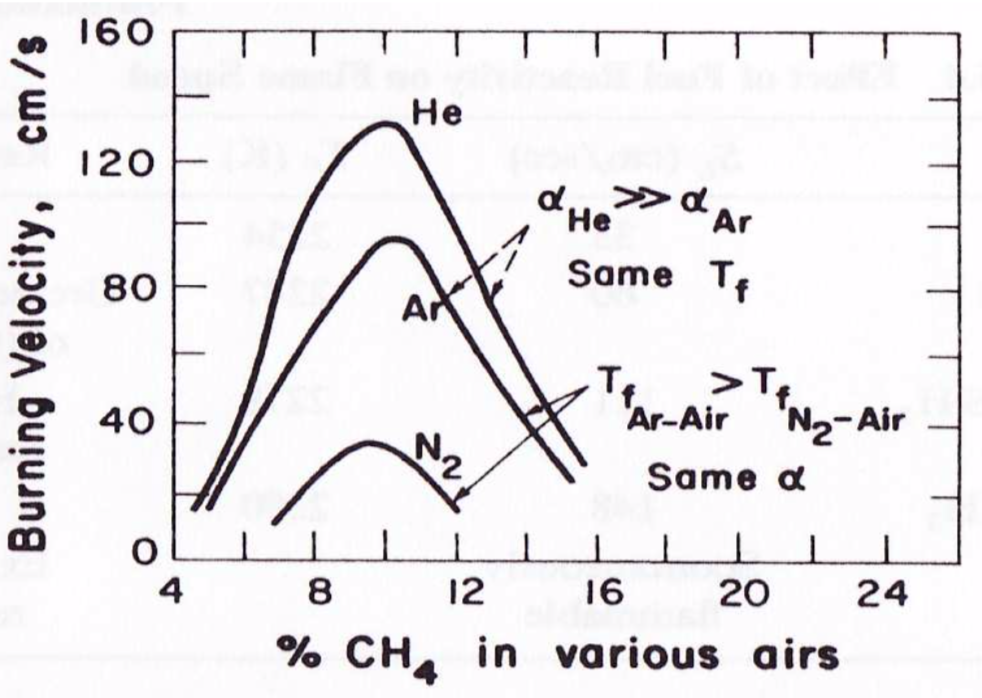
\includegraphics[width=0.6\textwidth]{figures/speed.png}
\end{figure}

\begin{itemize}
    \item $S_{L}$ in $He$ mixture is higher than $Ar$ mixtures. This is due to thermal diffusivity of $He$ which is much larger than that of $Ar$ (because weight of $He$ is much smaller). $He$ and $Ar$ are both monoatomic gas and thus their flame temperature are equal (they have same $C_{p}$).
    \item $S_{L}$ in $Ar$ mixture is higher than $N_{2}$ mixtures. This is due to lower specific heat of $Ar$ ($C_{p}=5/2R$ monoatomic) with respect to $N_{2}$ ($C_{p}=9/2R$ diatomic). But the flame temperature will be higher in the $Ar$.
\end{itemize}

Therefore, high values of $\alpha$ and low values of $C_{p}$ are key for a good burning rate.

\subsubsection{The Burke and Schumann model (D)}

Rather than considering a round jet, the jet is considered to be planar. The geometry is thus totally two-dimensional. Moreover, the jet and the sorrounding air have the same unit flow rate $\rho v$.

\begin{figure}[!ht]
\centering
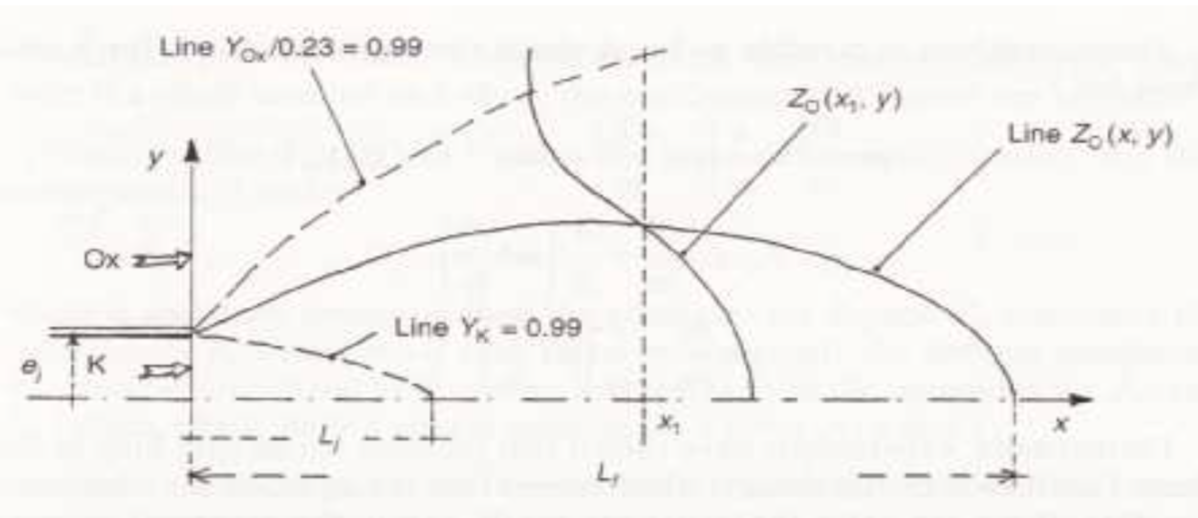
\includegraphics[width=0.8\textwidth]{figures/burke.png}
\end{figure}

Main assumptions:
\begin{itemize}
    \item Steady state
    \item Only three reactive species are present: the fuel ($K$), the oxidant ($Ox$) and the products ($P$).
    \begin{equation}
        K + vOx \rightarrow P
    \end{equation}
    where $v$ is the stoichiometric coefficient
    \item Three equations can be written for $Y_{i}$ where $i=K,Ox,P$
    \item Diffusion is the same: $D_{Ox}=D_{K}=D_{P}=d$
    \item Flow velocity is always parallel to the plane of symmetry, therefore the perpendicular equations are neglected.
\end{itemize}
Under these assumptions the equations are:

\begin{equation}
    \rho v\frac{\partial Y_{i}}{\partial x}=\frac{\partial}{\partial y}\bigg(\rho d \frac{\partial Y_{i}}{\partial y} \bigg) + \rho w_{i}, \text{\;}\text{\;}\text{\;} i=Ox, K, P
\end{equation}
\begin{equation}
    \rho v\frac{\partial h}{\partial x}=\frac{\partial}{\partial y}\bigg(\rho d \frac{\partial h}{\partial y} \bigg)
\end{equation}
\begin{equation}
    \rho v\frac{\partial v}{\partial x}=\frac{\partial}{\partial y}\bigg(\rho d \frac{\partial v}{\partial y} \bigg) - \frac{\partial p}{\partial x}
\end{equation}

Experiments have shown that pressure varies very little in the flame, which means that the last equation become obsolete. The remaining 4 differential equations require boundary conditions at $x=0$, $y=0$, $y=\infty$.\\
Note that since the reaction which consumes K and Ox, is the same as that which produces P, then the rates of reaction by mass for these species are related by their specific stoichiometric coefficients:
\begin{equation}
    \dot{\omega}_{Ox} = v_{s}\dot{\omega}_{K} \text{\;\;\;\;\;\;} \dot{\omega}_{P} = -\dot{\omega}_{K}
\end{equation}
where $v_{s}=v\frac{M_{Ox}}{M_{K}}$ is the mass stoichiometric coefficient.\\
Consequently, if two functions are defined $Z_{0}=Y_{K}-Y_{Ox}/v_{s}$ and $Z_{P} = Y_{K}+Y_{P}$, then these two functions satisfy the following differential equation, obtained as indicated in their definitions:
\begin{equation}
    \rho v\frac{\partial Z_{0}}{\partial x}=\frac{\partial}{\partial y}\bigg(\rho d \frac{\partial Z}{\partial y} \bigg)
\end{equation}
Such functions are called \textit{Schvab-Zeldovitch} functions and they exist only when the diffusion coefficients are the same. They satisfy the boundary conditions. Solving $Z_{0}(x,y)$ is now simply a question of mathematics.

\begin{figure}[!ht]
\centering
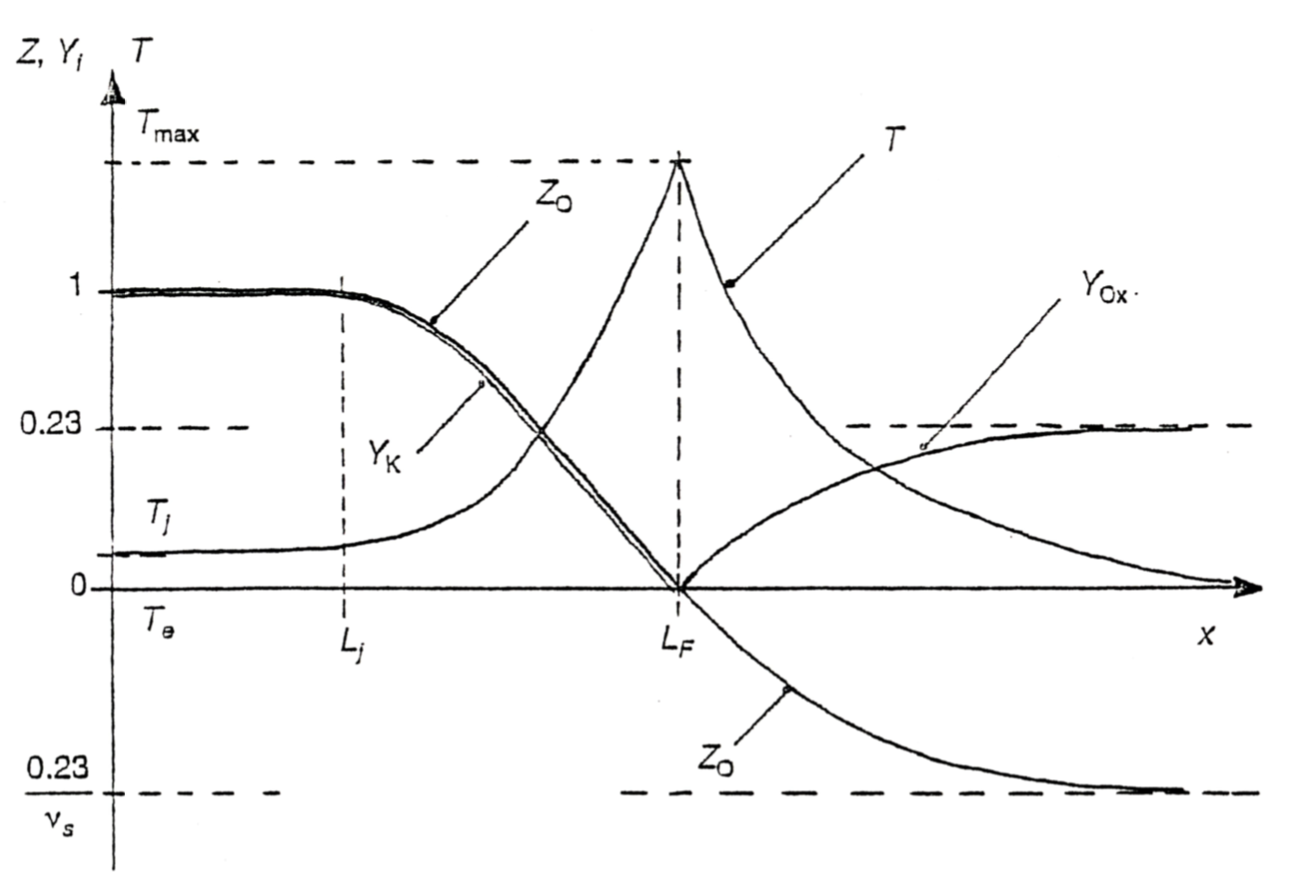
\includegraphics[width=0.6\textwidth]{figures/schumann.png}
\end{figure}

The length of the flame $L_{F}$ is inversely proportional to the diffusion coefficient and the greater is the jet velocity, the longer the flame is.

\subsection{Flame stability}

The stability of a combustion wave can be studied from a flame originated by a Bunsen burner. This is done by analyzing how the position of the flame changes with respect to the outflow section.

\begin{figure}[!ht]
\centering
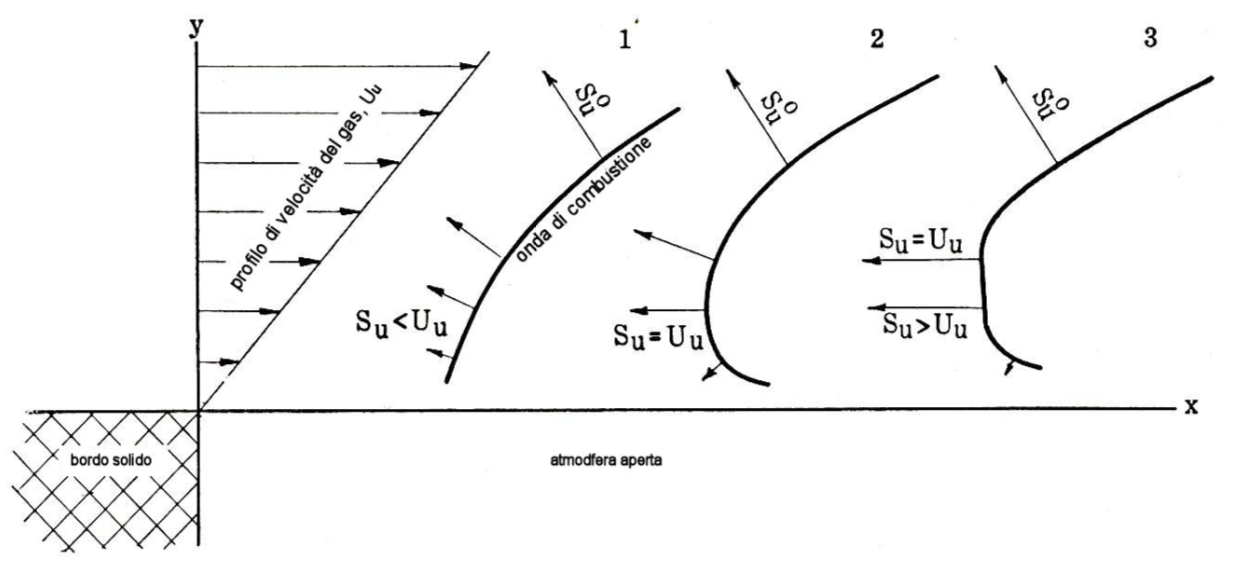
\includegraphics[width=0.6\textwidth]{figures/stability2.png}
\end{figure}

(flow is horizontal)
\begin{enumerate}
    \item combustion wave too close to solid rim. Jet velocity exceeds the flame velocity everywhere ($S_{u}<U_{u}$) and it is pushed back.
    \item equilibrium position ($S_{u}=U_{u}$). Due to the increased distance from the rim the burning rate increases but on the outer part the two velocities are equal.
    \item wave too far from the rim. In some points the flame velocity exceeds the jet and it moves forward toward the equilibrium position.
\end{enumerate}

\subsubsection{Flash-back and blow-off phenomena}

\begin{itemize}
    \item \textit{Flash-back}: upstrean propagation of the flame
    \item \textit{Blow-off}: downstream propagation of the flame
\end{itemize}
These conditions can be characterized by considering the jet and flame velocities and also the distance form the rim.
The parameters to look into to analyze these phenomena is the \textit{velocity gradient}.
We can distinguish the critical velocity gradient for flash-back and the critical velocity gradient for blow-off.

\begin{figure}[!ht]
\centering
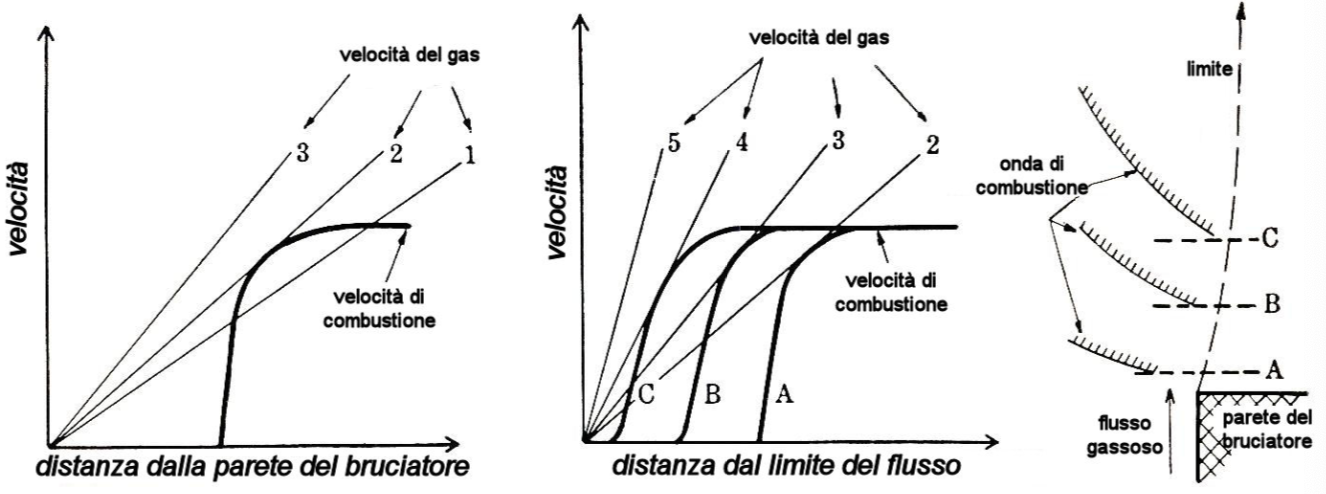
\includegraphics[width=0.9\textwidth]{figures/flash.png}
\end{figure}

\begin{enumerate}
    \item flash-back
    \item flash-back limit
    \item no flash-back
\end{enumerate}

\subsubsection{Quenching for natural gas-air mixtures}

\begin{itemize}
    \item \textit{Quenching}: the distance from the wall in which the flame is unable to propagate under the given conditions.
\end{itemize}
Due to heat transfer from the flame to the walls (which has higher thermal conductivity), temperature of the reaction zone gets lowered below ignition point and the flame gets extinguished.

\begin{figure}[!ht]
\centering
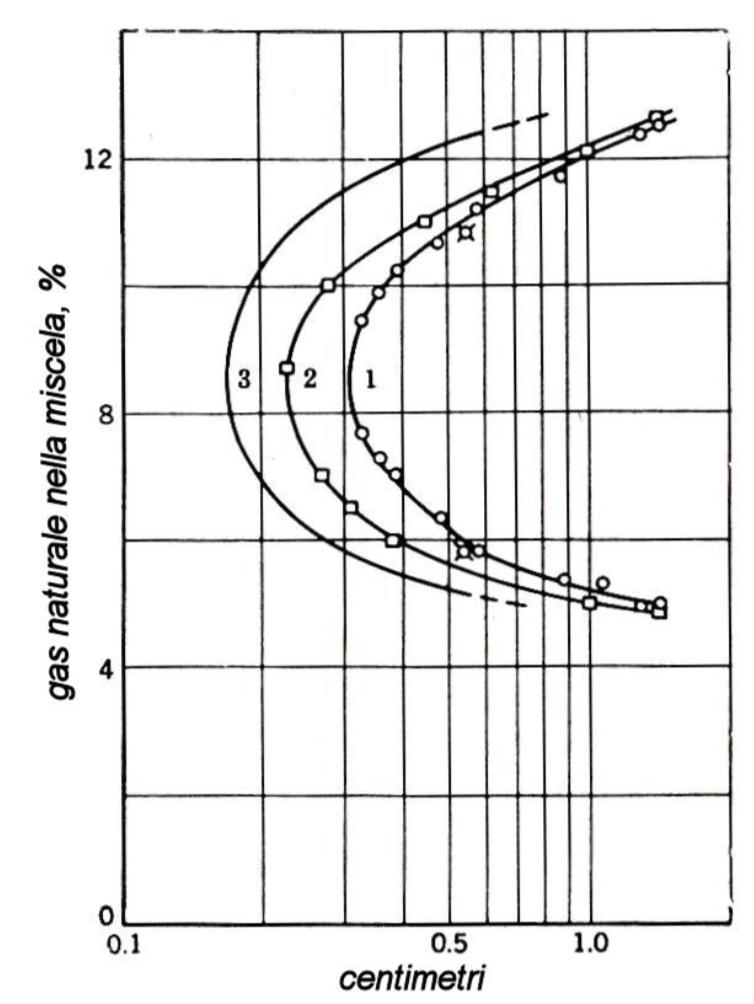
\includegraphics[width=0.4\textwidth]{figures/quenching.png}
\end{figure}

\begin{enumerate}
    \item quenching of cylindrical tubes
    \item quenching between plane-parallel plates
    \item depth of penetration from critical velocity gradient for flash-back
\end{enumerate}

\subsubsection{Characteristic regions of flame stability}

Flame stability is usually characterized by lift-off velocity, lift-off height and blow-out velocity:

\begin{itemize}
    \item \textit{lift-off velocity}: the mean jet velocity at which the flame becomes lifted from the rim exit
    \item \textit{lift-off height}: the distance between the lifted(!) flame base and the rim exit
    \item \textit{blow-out velocity}: the jet velocity at which the reaction cannot be sustained and the flame is extinguished
\end{itemize}

The stability limits of turbulent jet diffusion flames are important for operation of combustion systems and have safety implications. The lift-off and blow-out behaviors have been subject of numerous research efforts to allow the combustion within the stability limits.

\begin{figure}[!ht]
\centering
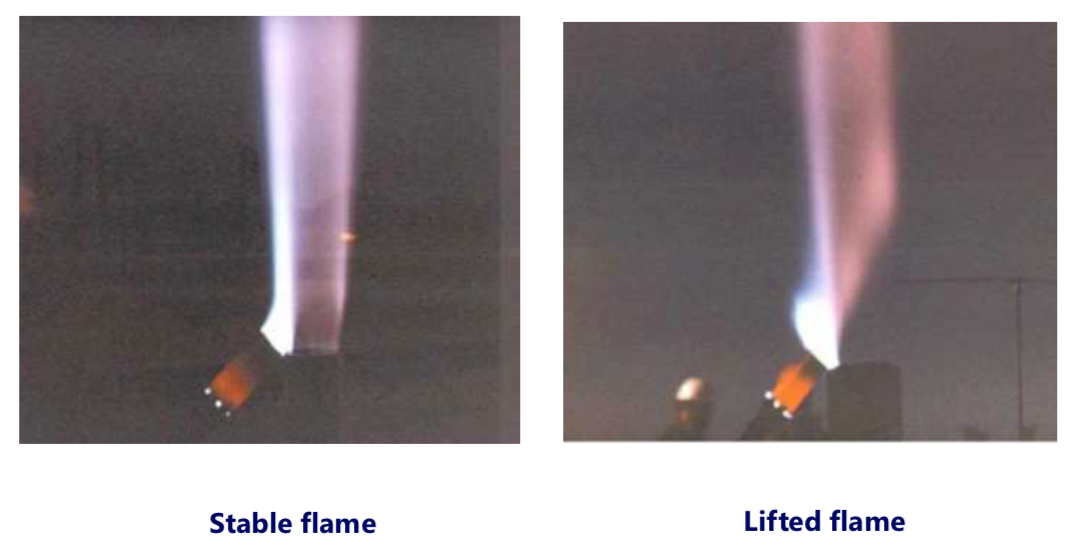
\includegraphics[width=0.5\textwidth]{figures/stableflame.png}
\end{figure}

\begin{itemize}
    \item Stable flame: firmly anchored at the rim exit
    \item Lift-off: permanent separation of the flame from the rim exit
\end{itemize}

\newpage

\section{Ignition and extinction phenomena}

Ignition is a transition from a nonreactive to a reactive state characterized by a self-sustained combustion.\\
The reason for studying ignition is to achieve basic understanding of the detailed process involved. Ignition involve many physical and chemical steps and it is a transient phenomena. Detailed chemical kinetics are used to predict ignition. The usual conditions for ignition are given by a "3T" rule of thumb:

\begin{itemize}
    \item \textit{Temperature}: must be high enough to cause reactions
    \item \textit{Time}: must be long enough enough to allow the heat to be absorbed
    \item \textit{Turbulence}: muste be high enough so that there is good mixing between fuel and oxidizer
\end{itemize}

There are various means of achieving ignition. External stimuli can be classified into:

\begin{itemize}
    \item \textit{thermal energy stimuli}: transfer of energy to the reactants by conduction, convection or radiation
    \item \textit{chemical stimuli}: introduction of \textit{hyoergolic} reactive agents
    \item \textit{mechanical stimuli}: impact, friction or shock wave
\end{itemize}

\subsection{Ignition temperature}

The concept of "ignition temperature" can be inappropiate because the chemical reaction rate is nonzero for all temperatures according to Arrhenius equation. However this concept is still useful.

\begin{itemize}
    \item \textit{van't Hoff ignition temperature}: the temperature at which the rate of heat loss due to conduction is equal to the rate of heat production by chemical reactions
\end{itemize}

\subsection{The thermal ignition}

The rate of heat evolution $q_{r}$ due to chemical reaction in a chamber volume $V$ can be expressed as:
\begin{equation}
    q_{r}=\Delta H_{r} V \dot{\omega} = H_{r} V \bigg[Ae^{\frac{-E_{a}}{R}T} \pi C_{i}^{v_{i}}\bigg]
\end{equation}
where $\Delta H_{r}$ is the heat of reaction and $\dot{\omega}$ is the reaction rate.\\
The rate of heat loss to the walls of a vessel having surface $S$, radius $r_{p}$ and temperature $T_{W}$ can be written as:
\begin{equation}
    q_{L} = -S \lambda \bigg(\frac{\partial T}{\partial r}\bigg) \approx S \lambda\bigg[\frac {(T-T_{W})}{L}\bigg]
\end{equation}
where $\lambda$ is the thermal conductivity and $L$ is the characteristic thickness of the thermal layer near the wall.\\
Both equation depend on the geometry of the vessel, therefore the ignition temperature from these quations will depend upon the geometry.

\begin{figure}[!ht]
\centering
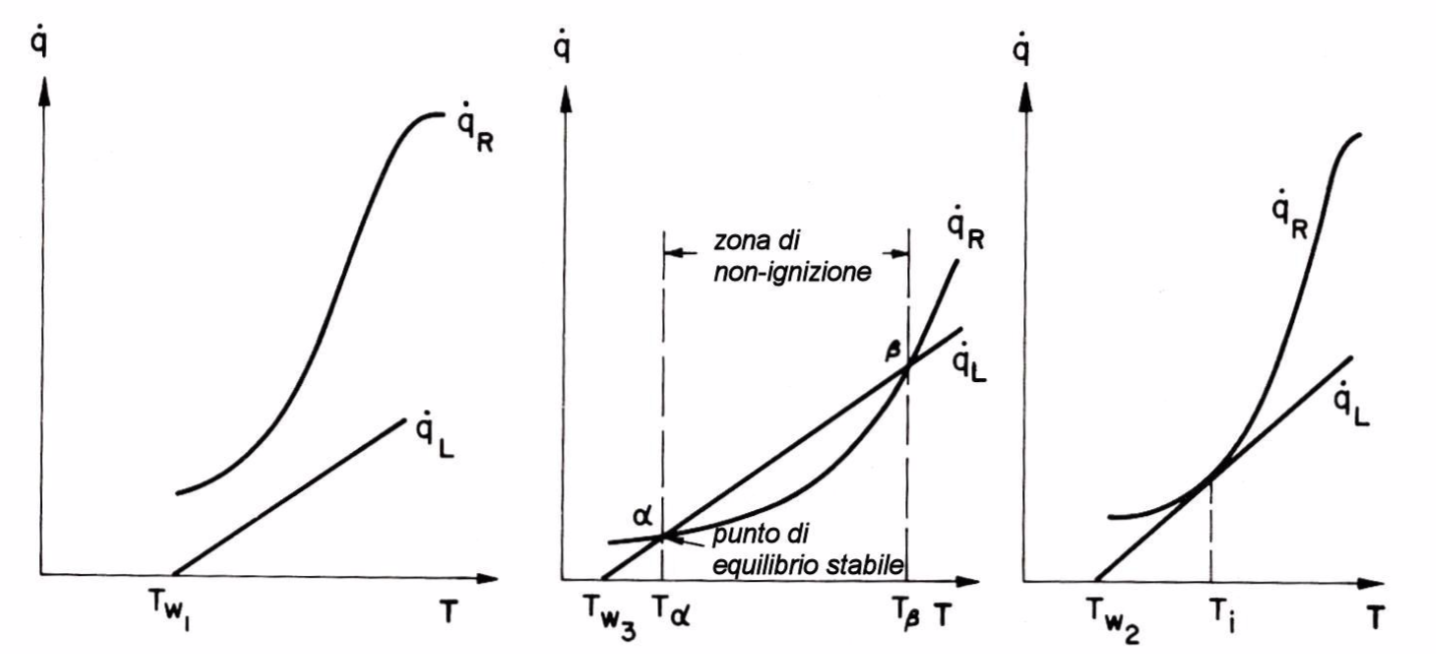
\includegraphics[width=0.6\textwidth]{figures/thermallossgain.png}
\end{figure}

This picture shows the relationship between the heat developed and the heat lost by a mixture in a vessel with temperature controlled walls:

\begin{itemize}
    \item \textit{(left)} the $T_{W}$ is high enough to cause immediate chemmical reactions, in this case $q_{r}$ is always greater than $q_{L}$.
    \item \textit{(center)} the $T_{W}$ is low enough to allow the heat generation by chemical reaction to be significant and the profile of $q_{r}$ near $T_{W}$ is flat. $q_{r}$ intersects $q_{L}$ at $T_{\alpha}$ and $T_{\beta}$. $T_{\alpha}$ is a stable equilibrium point since the mixture will self-heat to $T_{\alpha}$ but no further because $q_{L}$ is greater.
    \item \textit{(right)} the $q_{r}$ curve is tangent to $q_{L}$ at the ignition temperature $T_{i}$. This implies that after the reactants have been introduced into the vessel, they will self-heat to $T_{i}$. $T_{i}$ can be defined mathematically by equating the 2 slopes at the tangent point:
    \begin{equation}
        T_{i}=T_{W}+\bigg(R\frac{T_{W}^{2}}{E_{a}}\bigg)
    \end{equation}
\end{itemize}

\subsection{Effect of various parameters on $T_{i}$}

The effect of chamber volume can be seen from the following figure:

\begin{figure}[!ht]
\centering
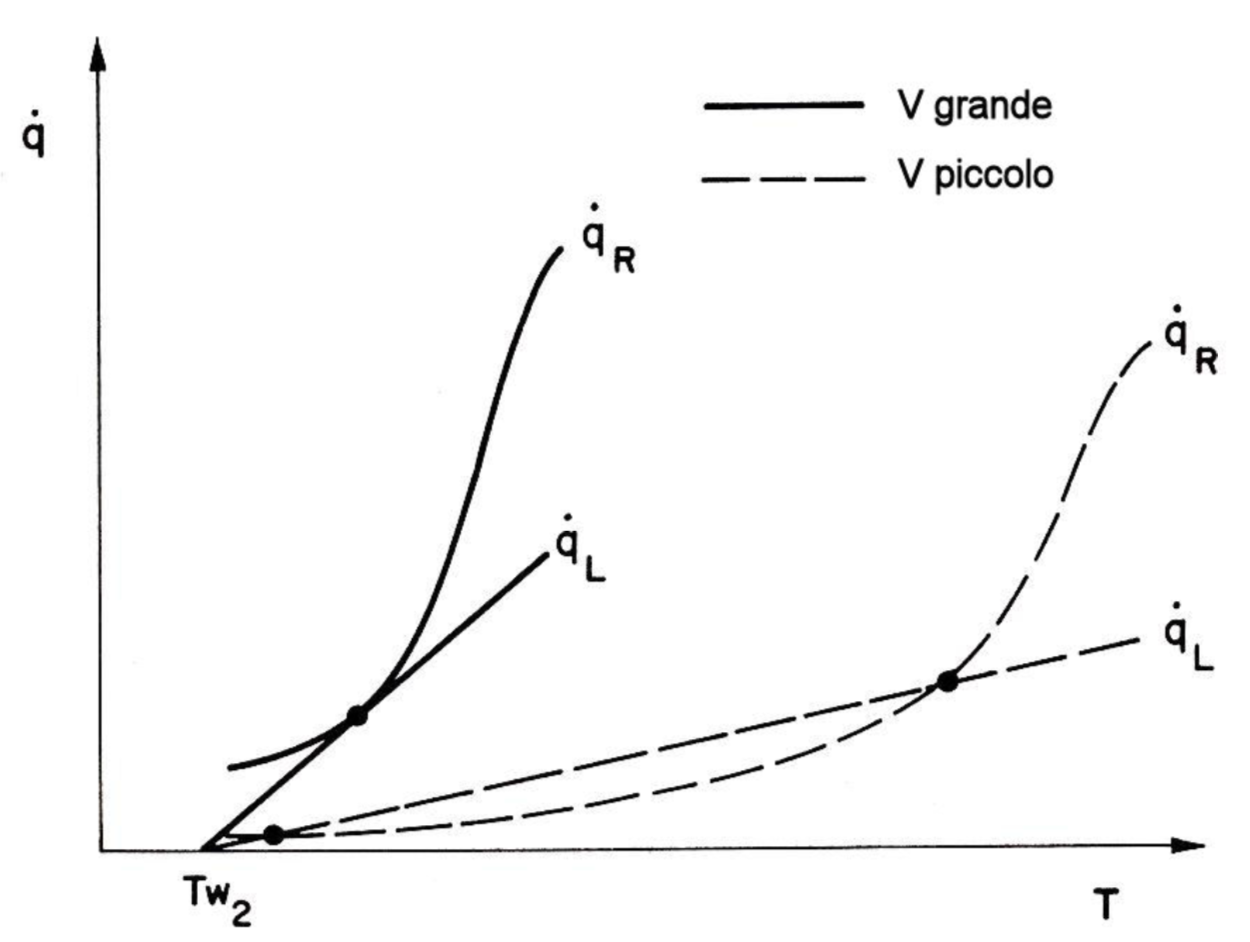
\includegraphics[width=0.5\textwidth]{figures/dashed.png}
\end{figure}

The dashed lines, corresponding to a smaller chamber, show no spontaneous ignition when wall temperature is $T_{W2}$. Thereforem it shows that by decreasing the volume, an ignitable system becomes not ignitable. This is due to the increase of heat loss and reduction of heat developed (see figure).\\
The reactant composition also has an effect on $T_{i}$ since $q_{r}$ is a function of the reaction rate which depends on the composition.\\
In general, $T_{i}$ is a function of:

\begin{itemize}
    \item the size of the apparatus
    \item the initial temperature of the mixture
    \item the reactant composition
    \item the activation energy
    \item time, pressure and turbulence
\end{itemize}

\subsection{Ignition of solid propellants}

The process of combustion of a solid substance involves a more complex analysis:

\begin{itemize}
    \item transfer of energy by conduction, convection or radiation
    \item in-depth energy absorption (inert heating)
    \item decomposition of solid phase, pyrolysis of fuel binder
    \item diffusion of species from the surface
    \item heterogeneous reaction between gaseous species and condensed phase
    \item abrupt increase of temperature
    \item emission of light from the reaction zone
\end{itemize}

\begin{figure}[!ht]
\centering
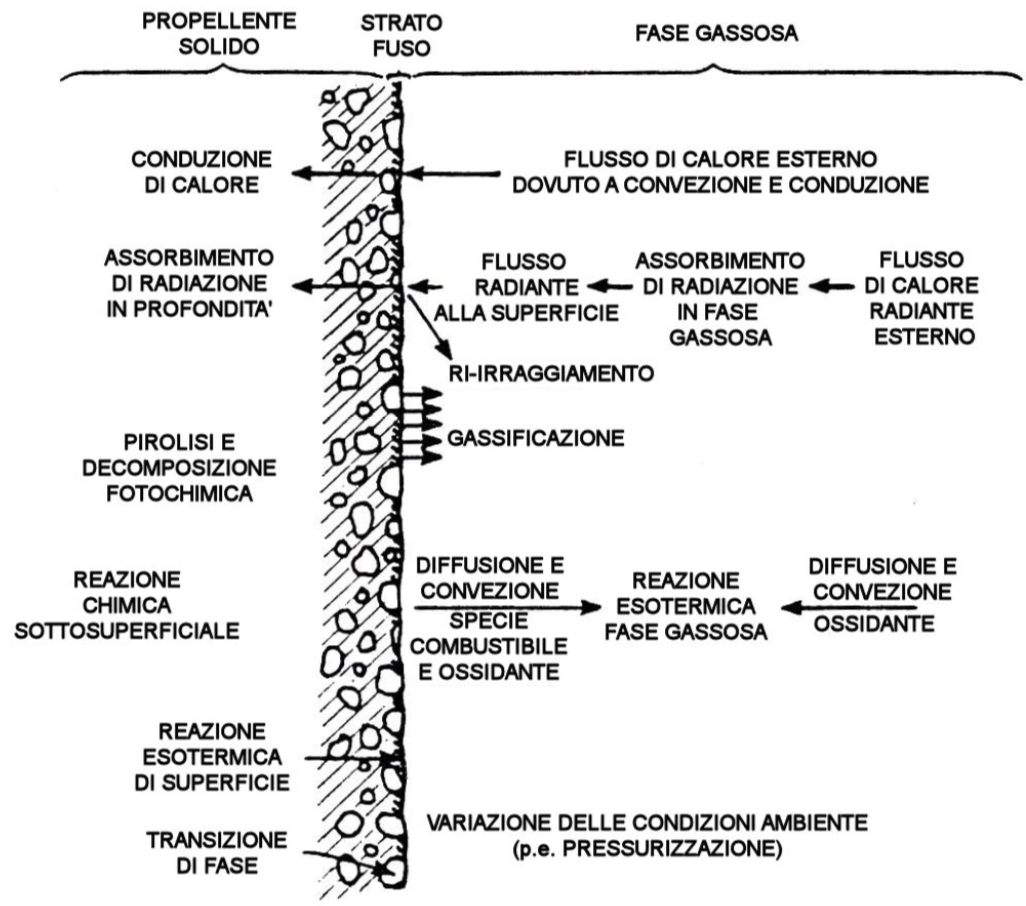
\includegraphics[width=0.6\textwidth]{figures/solid.png}
\end{figure}

\subsection{Ignition phenomena}

When the net heat involved overcomes heat losses, sustained ignition is achieved. Ignition is incomplete of combustion does not follow the ignition event after the removal of stimulus. The time period from the start of the stimulus to the instant of sustained ignition is called the \textit{ignition delay}.\\
Ignition theories are classified into 3 groups:

\begin{itemize}
    \item \textit{gas phase}: considers the ignition process to be controlled by the reaction between the fuel and oxidizer mixtures and the ambient oxidizer gases
    \item \textit{heterogeneous}: considers the reaction between the solid-phase fuel and ambient oxidizer at the interface
    \item \textit{solid-phase}: does not consider heat release and mass diffusion in the gas phase. The temperature rise inside a solid propellant is achieved by the heat release caused by subsurface reactions or external heating.
\end{itemize}

Within the 3 theories described above, several models have been proposed. These models differ in the governing equations considered, assumptions made, ignition criteria and type of propellants studied.

\subsection{Explosion limits}

\begin{figure}[!ht]
\centering
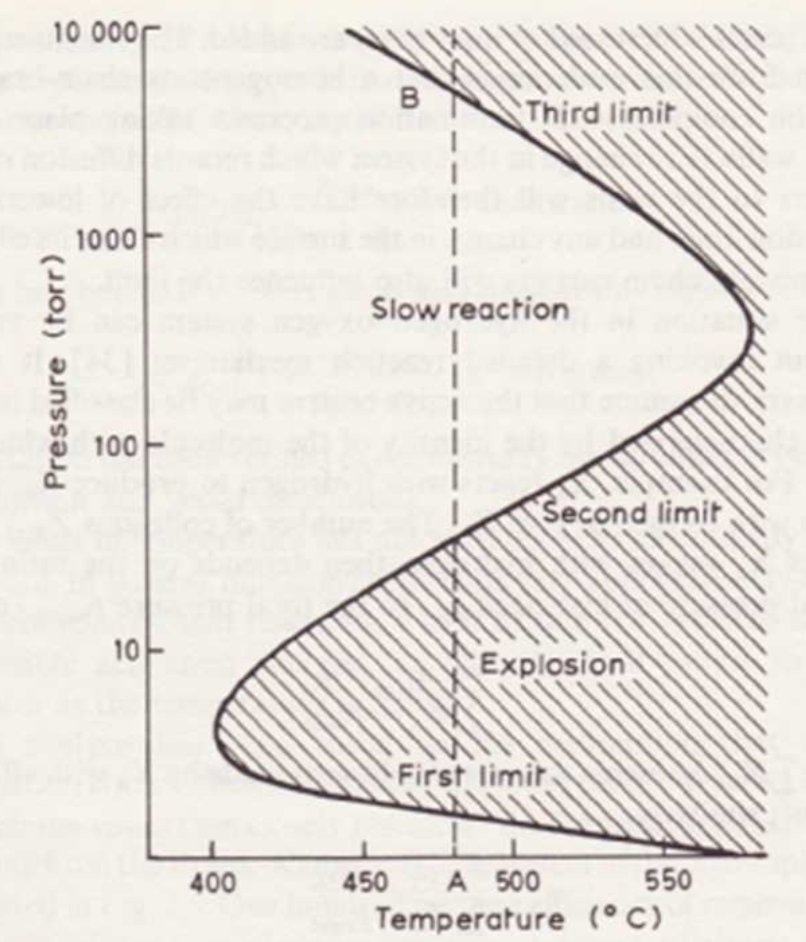
\includegraphics[width=0.4\textwidth]{figures/explosion.png}
\end{figure}

\begin{itemize}
    \item \textit{First limit}: the lower limit is affected by the nature of the surface coating of the container
    \item \textit{Second limit}: this limit is considered at higher pressures. At this limit, an increase in pressure inhibits the explosive reaction
    \item \textit{Third limit}: the rate of reaction is usually quite high immediately below the third limit and the characteristic observed tend towards those associated with thermal explosion
\end{itemize}

\subsection{Ignition of keresone sprays}

\begin{figure}[!ht]
\centering
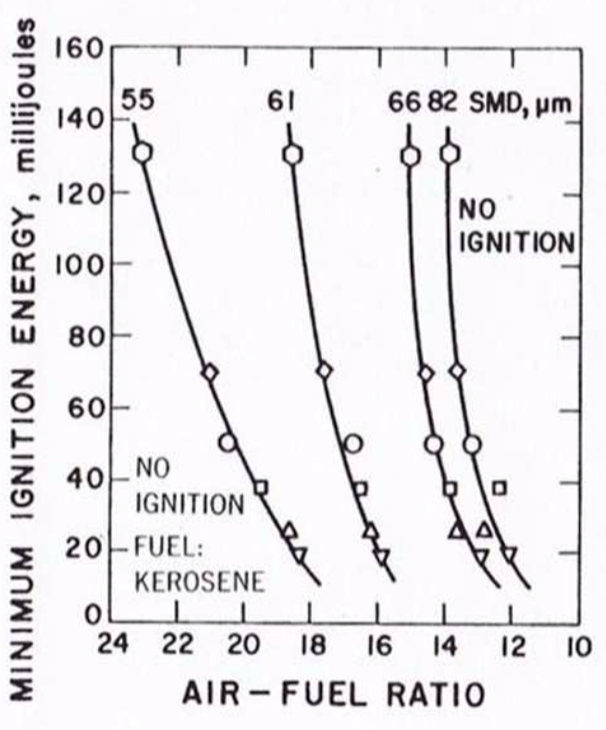
\includegraphics[width=0.3\textwidth]{figures/kerosene.png}
\end{figure}

The minimum ignition energy is plotted for 4 different values of the mean drop size. For each curve the left-hand size represents a region of no ignition and the right-hand size a region of ignition. This figure shows how the weak-ignition limit is improved by a reduction of drop size. The curves become steeper with increasing the drop size which indicates that a much greater increase in spark energy is needed.

\begin{figure}[!ht]
\centering
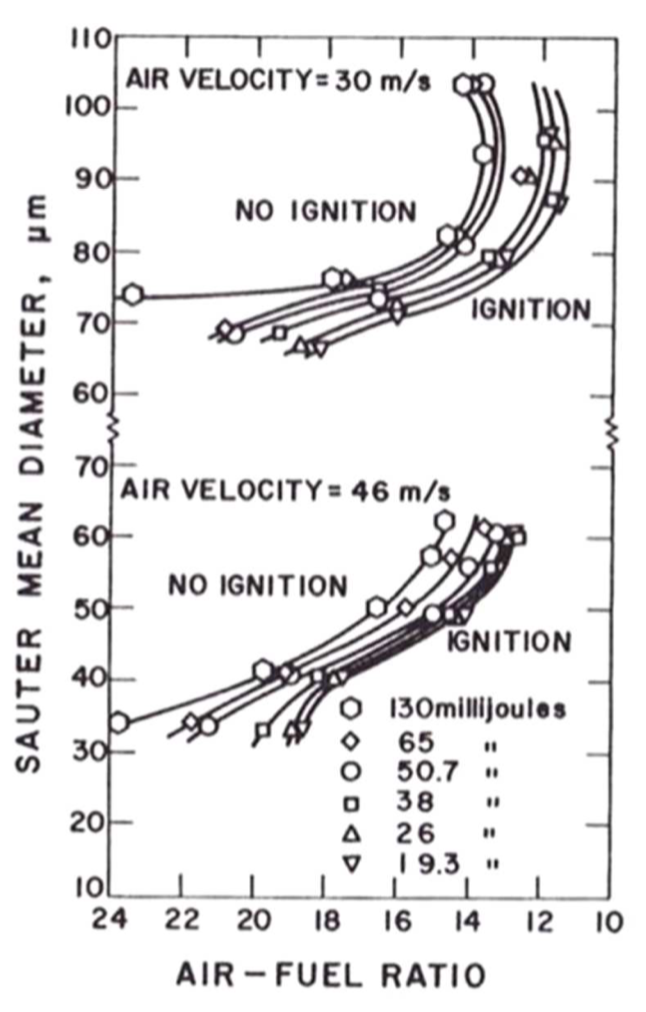
\includegraphics[width=0.3\textwidth]{figures/kerosene2.png}
\end{figure}

In this figure the ignition limits obtained at 2 different air velocities are plotted in terms of \textit{SMD} (sauter mean diameter - average of particle size) vs air-fuel ratio. For both velocities the weak-ignition limits are widened by an increase in spark energy. As the air-fuel ratio is reduced towards the stoichiometric value ($14.8$), the more rapid reaction releases more heat that allows further fuel evaporation and extend the ignition limits into a region of larger drop sizes.

\begin{figure}[!ht]
\centering
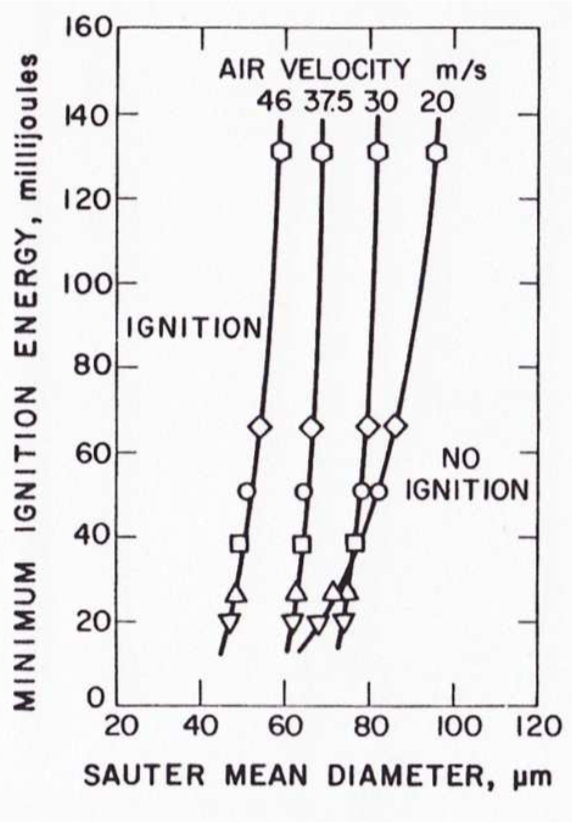
\includegraphics[width=0.3\textwidth]{figures/kerosene3.png}
\end{figure}

The figure shows the variation of minimum ignition energy vs the SMD for stoichiometric mixtures at 4 velocities. At all values of velocity, large increases in spark energy are needed to compensate for quite modest increase in drop size. This figure illustrates the crucial role of the fuel injector in the attainment of good ignition performance. Moreover improvements in the atomization during the ignition and minimization of the flow velocity (reduction of speed is good) in the ignition zone can significantly enhance ignition of sprays in flowing air streams.

\subsubsection{Minimum ignition energy}

The least amount of energy required from an external source to create such a spark whose size is equal to the quenching distance is defined as the \textit{minimum ignition energy $E_{min}$}:

\begin{equation}
    E_{min} = C_{p, air}\rho_{air}\Delta T_{stoich} \frac{\pi}{6}d_{q}^{3}
\end{equation}

the results of these experiments show that the most important parameters affecting $E_{min}$ are drop size, air velocity and fuel-air ratio. In particular, even a slight improvement in atomization quality decreases $E_{min}$ and is beneficial to ignition.

\newpage

\section{Two-phase flow combustion}

\subsection{Droplet combustion}

The simplest case to study is not that of a drop whose diameter reduces as it burns, but rather that of a drop which is fed with fuel at its center so the diameter remains constant. With this arrangement the problem is stationary, the flame and the drop can be described with one spatial variable, the distance from the center of the drop.\\
The combustion of a single droplet is studied using the double-film model. One film separates the droplet surface from the flame front, and the other separates the flame from the sorrounding oxidizer.

\begin{figure}[!ht]
\centering
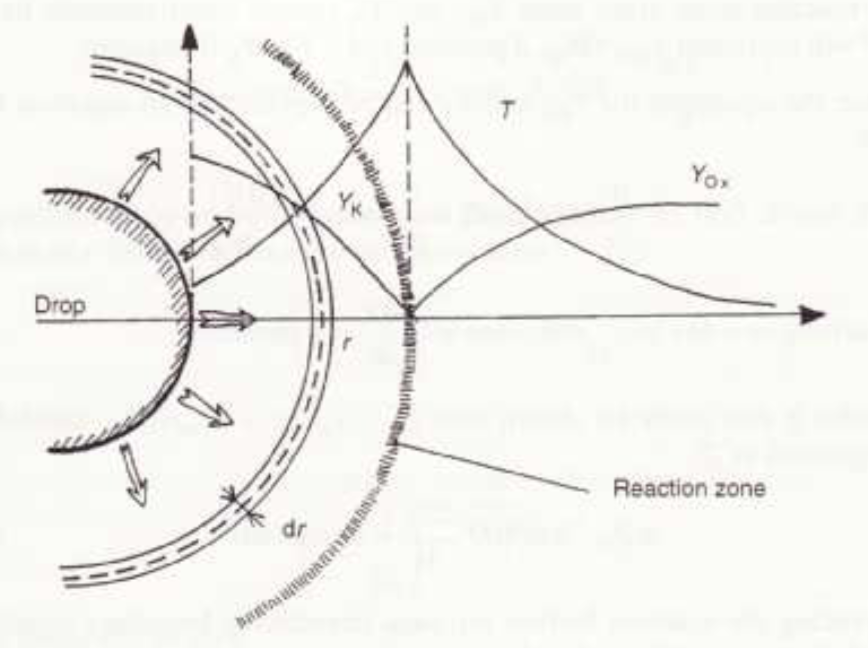
\includegraphics[width=0.5\textwidth]{figures/droplet.png}
\end{figure}

The solution of this problem is performed using the following assumptions:

\begin{itemize}
    \item pressure is constant
    \item the drop is at uniform temperature
    \item the $C_{p}$ for the gas is constant
    \item an infinitely rapid chemical reaction of the type $K+vOx \rightarrow P$ occurs
    \item the coefficient of molecular diffusion for $Ox$ and $K$ are all equal to $D$, and $\rho D$ can be assumed constant
\end{itemize}

The most important parameter to consider is the \textit{mass burning rate} since it permits the evaluation of the \textit{evaporation coefficient}.

\subsubsection{The evaporation coefficient}

The evaporation coefficient $\beta$ is defined by the following $d^{2}$ evaporation law:
\begin{equation}
    d^{2}=d_{0}^{2}-\beta_{0}t
\end{equation}
where $d_{0}$ is the original drop diameter, amd $d$ the drop diameter after time $t$.\\
We are interested in the rate of regression of he condensed material (mass consumption). The condensed phase must be gasified, and consequently there must be an energy input into the condensed material. The heat of flux at the surface determines the rate of regression:
\begin{equation}
    q_{s}=r\rho_{liq}Q
\end{equation}
(s: surface)
\begin{itemize}
    \item $q_{r}$ is the heat flux to the surface
    \item $r$ is the regression rate
    \item $Q$ is the energy required to bring the material to the temperature of vaporization
\end{itemize}

\subsubsection{Evaporation of a single fuel droplet}

The fuel \textit{evaporation rate} expression can be written as:
\begin{equation}
    G_{F}=\frac{\dot{m}_{F}}{4\pi r_{s}^{2}}=\rho_{s}\mathcal{D}_{s}\frac{ln(1+B)}{r_{s}}
\end{equation}
 where $B$ is called the \textit{Spalding transfer number}:
 \begin{equation}
     B=b_{\infty}-b_{s}=\frac{Y_{Fs}-Y_{F\infty}}{1-Y_{Fs}}
 \end{equation}
 The value of $B$ must be evaluated in order to calculate the mass evaporation rate. Before that, $Y_{F}$ (fuel mass fraction) or $p_{F}$ must be determined, but the gas which sorrounds the droplet is saturated by the vapor or liquid of the droplet at the surface. Thus the problem becomes to determine $T_{d}$ since pressure data are available.\\
 The time of evaporation of a liquid droplet is an important parameter in combustion chamber design since the lifetime of the largest droplet in a spray determines the minimum time the droplet must be allowed to reside in the combustion chamber.

\begin{figure}[!ht]
\centering
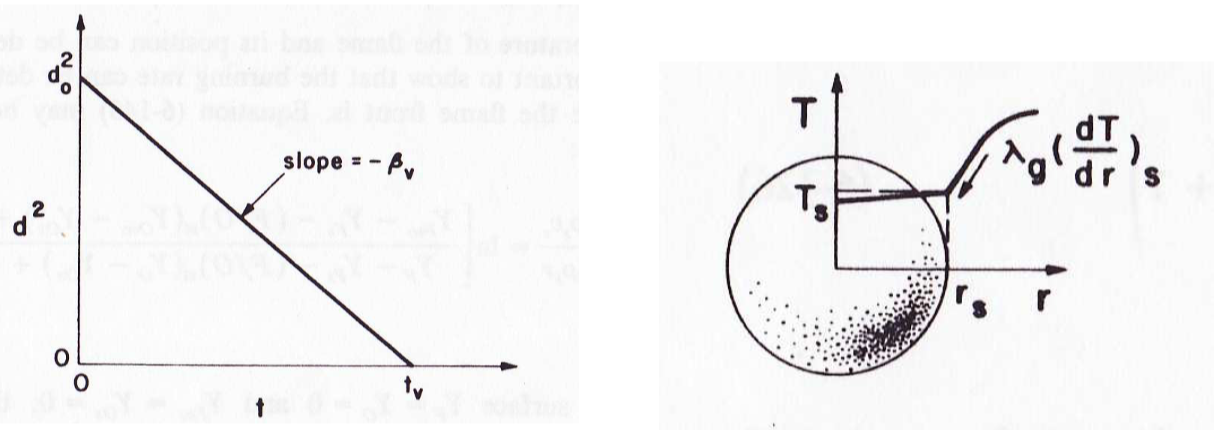
\includegraphics[width=0.8\textwidth]{figures/droprate.png}
\end{figure}

\begin{itemize}
    \item (left) the $d^{2}$ evaporation law for liquid fuel droplets. Note that the evaporation coefficient $\beta$ represents the magnitude of the negative slope
    \item (right) the temperature distribution of an evaporating liquid droplet
\end{itemize}

\begin{figure}[!ht]
\centering
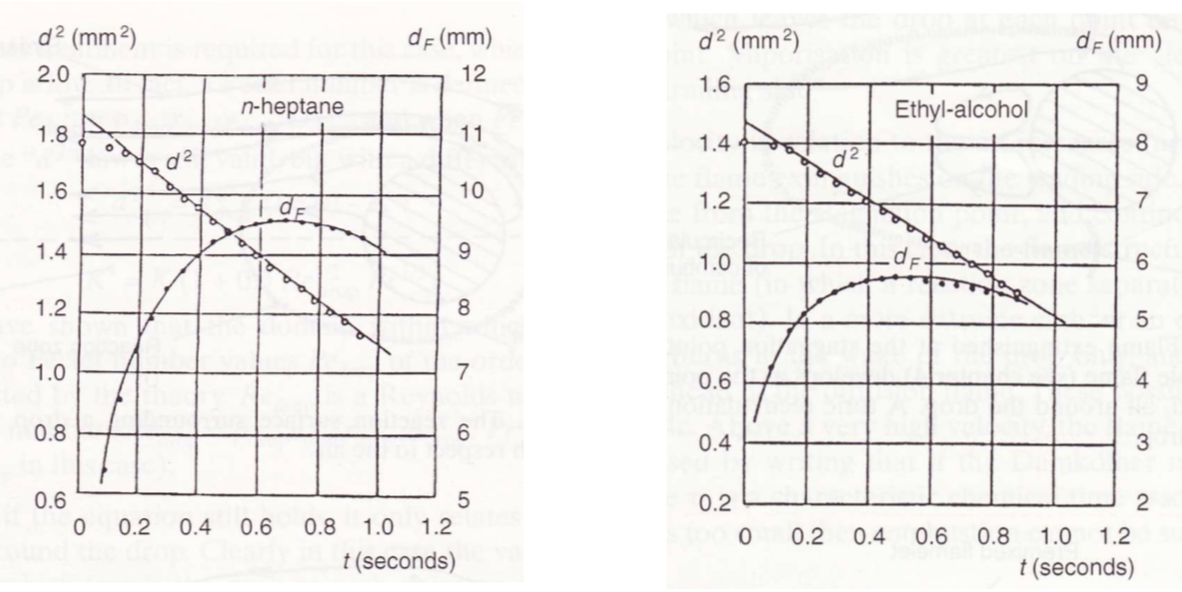
\includegraphics[width=0.8\textwidth]{figures/flamediameter.png}
\end{figure}

Note that the ratio $\frac{r_{F}}{r_{drop}}$ ($r_{F}$ is the radius of flame) assumed to be constant in the steady-state theory, varies greatly as the drop burns. This is apparent in the figure which plots the diameters.

\subsubsection{Combustion of a single fuel droplet}

In a single droplet burning analysis we assume that the fuel and oxidant depletion rates are related in stoichiometric proportions:
\begin{equation}
    \dot{\omega}_{F} = \dot{\omega}_{0}(F/O)_{stoich}
\end{equation}

TODO

\subsection{Spray combustion systems}

Spray combustion occurs in liquid rocket engines, gas turbines, diesel engines. The predictive models for spray combustion processes becomes important. A realistic analytical model of a combusting spray must involve consideration of several phenomena such as:
\begin{itemize}
    \item spray formation and transport characteristics of individual droplets
    \item turbulent two-phase flow
    \item interactions of radiation with flame turbulence
\end{itemize}

Sprays are burned in various ways, and each poses different problems:

\begin{figure}[!ht]
\centering
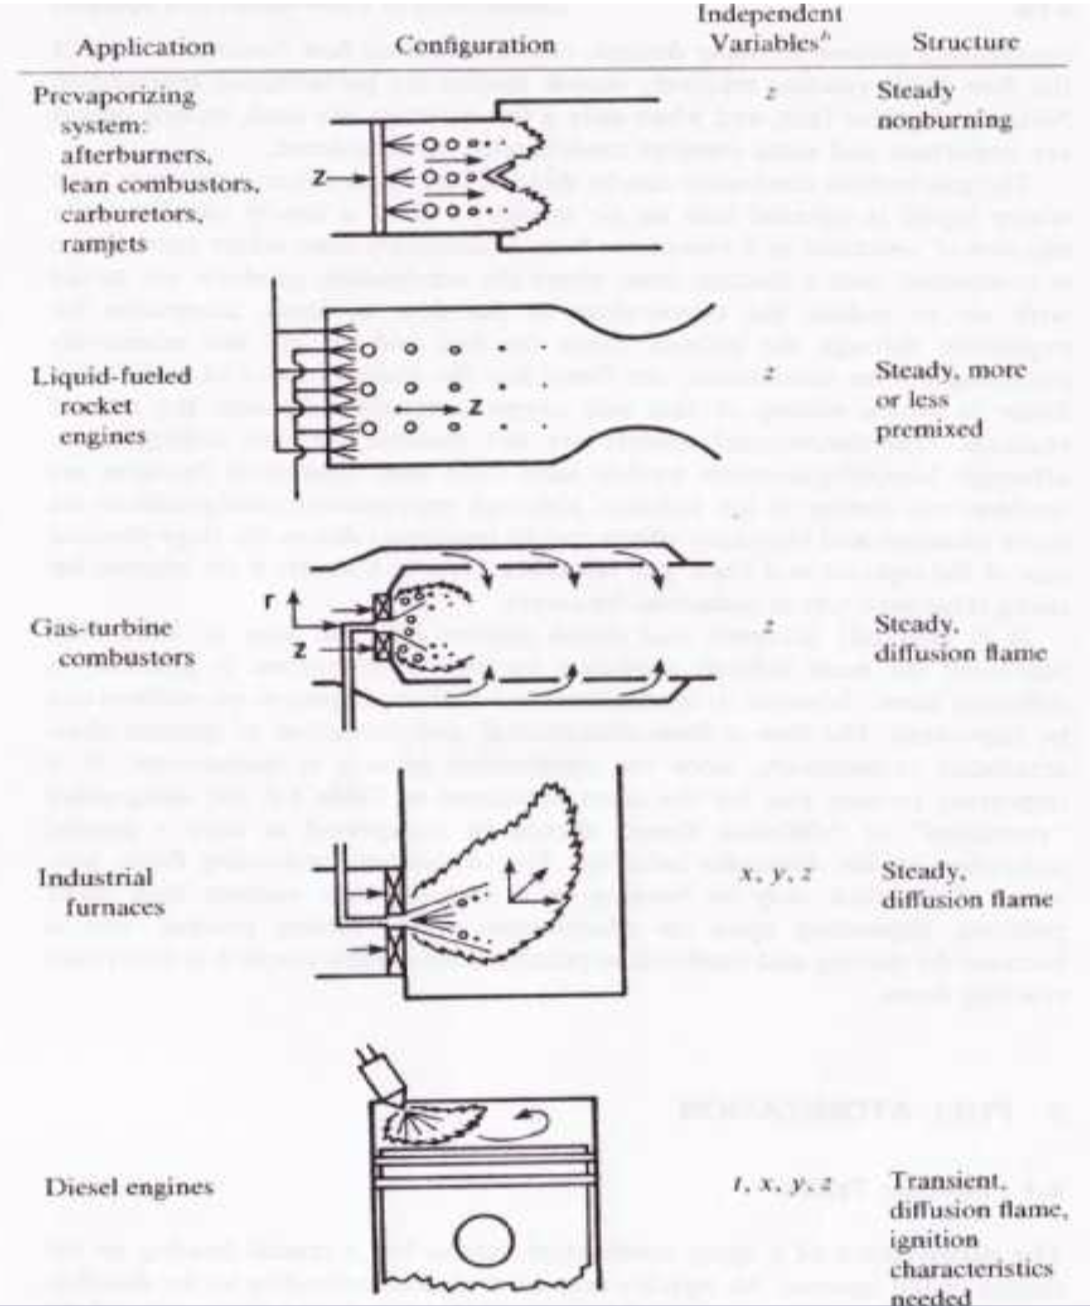
\includegraphics[width=0.4\textwidth]{figures/spraycomb.png}
\end{figure}

\begin{itemize}
    \item \textit{prevaporizing system}: the spray is injected in a heated air stream and the drops are almost completely evaporated before reaching the flame (afterburners)
    \item \textit{liquid rocket engines}: both fuel and oxidizer are injected from one end, providing a more or less premixed
    \item \textit{gas turbine combustor}: the fuel and air are not extensively premixed before combustion, the flame has the characteristics of a diffusion flame
    \item \textit{industrial furnaces}: similar to gas turbines
    \item \textit{diesel engines}: the process is primarily a diffusion flame, prediction is necessary since the combustion process is intermittent
\end{itemize}

\subsubsection{Fuel atomization}

Injectors can be classified into 2 categories:

\begin{itemize}
    \item \textit{pressure-atomizing injectors}: atomization is achieved by pressure drop
    \item \textit{twin-fluid injectors}: atomization of the liquid is aided by a flow at high velocity through injector passages
\end{itemize}


\subsubsection{Spray particles characterization}

The shape of liquid droplets may be considered to be spherical (can be characterized by only the radius) when the following 2 conditions are met:
\begin{enumerate}
    \item the collision and agglomeration effects are small, this requires that the volume occupied by the condensed phase be much less than the total spatial volume
    \item the \textit{Weber} number is low ($We<20$), the degree of deformation of a droplet caused by the slip velocity between the droplet and gas depends upon the ratio of the dynamic force to the surface-tension force:
    \begin{equation}
        We = \frac{dynamic force}{surface tension force} = 2r\rho_{gas}\frac{(v_{drop}-v_{gas})^{2}}{\sigma_{s}}
    \end{equation}
\end{enumerate}

\subsubsection{Drop size distribution}

Overall spray characteristic are represented by distribution curves which are given in terms of the cumulative percentage. In many processes it is desirable to work only with average diameters instead of the complete drop-size distribution.

\begin{figure}[!ht]
\centering
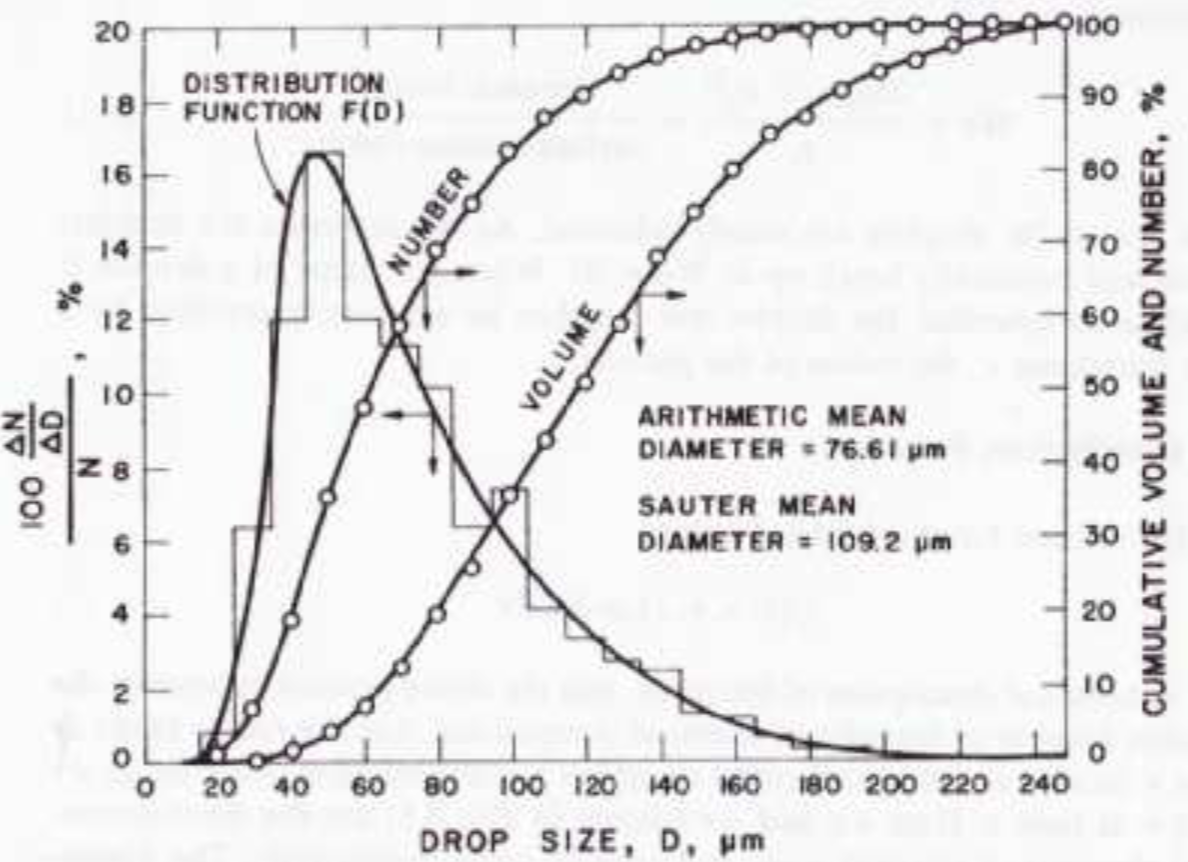
\includegraphics[width=0.4\textwidth]{figures/distribution.png}
\end{figure}

\subsubsection{Spray combustion characteristics}

Although combustion of droplets in a spray in governed by the diffusion of fuel vapor and oxidizer, both premixed and diffusion flame theories have been applied to spray combustion problems but for the former caution must employed.\\ For both cases, it must be considered the size and volatily of the droplet since for very small droplets of a high-volatily fuel, the droplet evaporation may be completed in the heat-up process, so that the flame structure is not influenced by the two-phase flow.

\subsubsection{Spray and gas flame comparison}

Experiments on spray combustion flames of axial jets of kerosene show the region where the droplets exist is limited to a small area above the burner nozzle. It is concluded that most of the droplets in the flame do not burn individually but that fuel vapor from the droplets forms a cloud and burns like a gaseous diffusion flame.\\ Changing only the fuel from liquid kerosene to gaseous propane, the spray combustion flame was found to be very similar to the previous. It is obvious that there is a resemblance between the two cases. However in the gas diffusion flame, chemical reactions occured slightly downstream as compared with the spray one. This is due to higher flow velocity of propane than of kerosene. In the spray, the temperature drop in steeper than in the gas diffusion flame, the difference is caused by the higher radiation cooling rate of the spray combustion flame.

\begin{figure}[!ht]
\centering
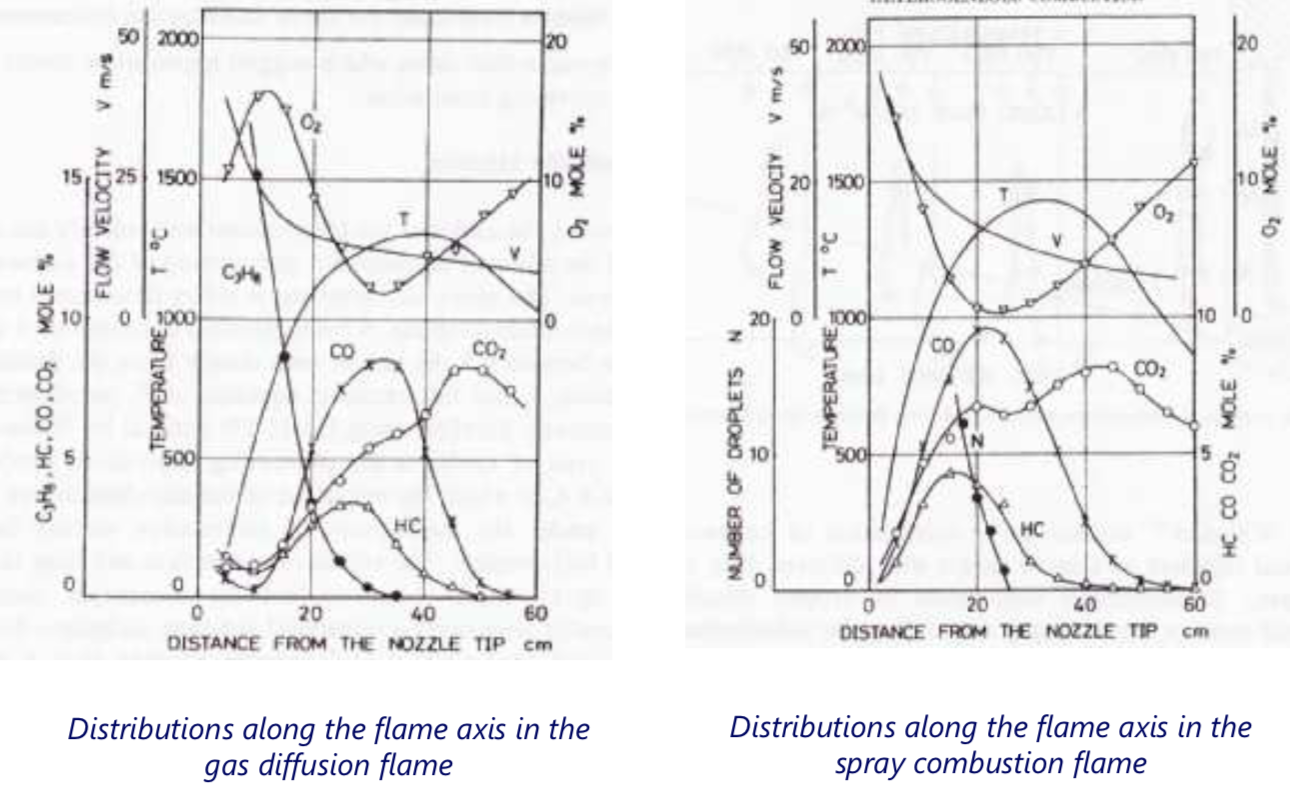
\includegraphics[width=0.6\textwidth]{figures/spraygas.png}
\end{figure}

\subsubsection{The spray combustion process}

\begin{figure}[!ht]
\centering
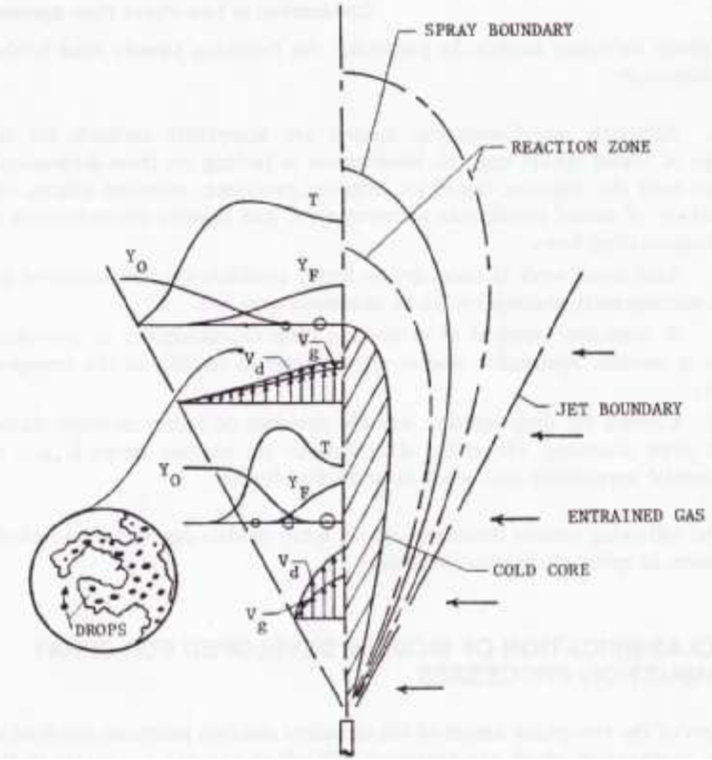
\includegraphics[width=0.5\textwidth]{figures/core.png}
\end{figure}

The figure illustrates the locations of the cold core region, reaction zone, spray boundary and jet boundary of a coaxial spray diffusion flame. The spray leaving the injector is highly nonuniform with smaller droplets at the periphery and larger droplets near the centerline. The outer small droplets evaporate rapidly to provide fuel vapor which is consumed near the outer portion of the turbulent diffusion flame. Larger droplets can travel long distance before evaporation and combustion processes begin, this is due to the high inertia. With increasing distance from the injector exit, the centerline temperature increases due to combustion of the spray. Experiments show that the disappearance of droplets is correlated with positions of maximum temperature, instead fuel evaporation occurs in relatively cool regions.

\subsection{Spray combustion in a Diesel reciprocating engine}

The goal is to develop predictive combustion models for diesel engines. Today, models are able to predict the \textit{ignition delay} including $NO$ and $soot$ emissions. Diesel combustion models can be classified into 2 groups:
\begin{enumerate}
    \item \textit{thermodynamic models}: aim to calculate the heat release rate according to a given pressure history
    \item  \textit{multidimensional models}: are based on the evaluation of the fluid dynamic properties such as temporal and spatial variations, composition, pressure and turbulence. They are more predictive and can provide more fundamental information of the combustion phenomena
\end{enumerate}

\subsubsection{KIVA-II}

KIVA-II is a program devoted to the numerical calculation of transient, 2 and 3-dimensional reactive fluid flows with sprays. A stochastic particle model is used to calculate evaporating liquid sprays, including the effects of droplet collisions.\\
The in-cylinder dynamics of internal combustion engines involve complex physical and chemical processes. These include the transient 3-dimensional dynamics of evaporating fuel sprays, chemical reactions and heat transfer. The KIVA code has the ability to calculate such flows with arbitrarily shaped piston geometries and it solves the unsteady equations of motion of the reactive mixture coupled to the equations for a single component vaporizing fuel spray.\\
The KIVA equations can be used to solve both laminar and turbulent flows which differ primarily in the form and magnitude of the transport coefficients (much larger in the turbulent case).

\begin{figure}[!ht]
\centering
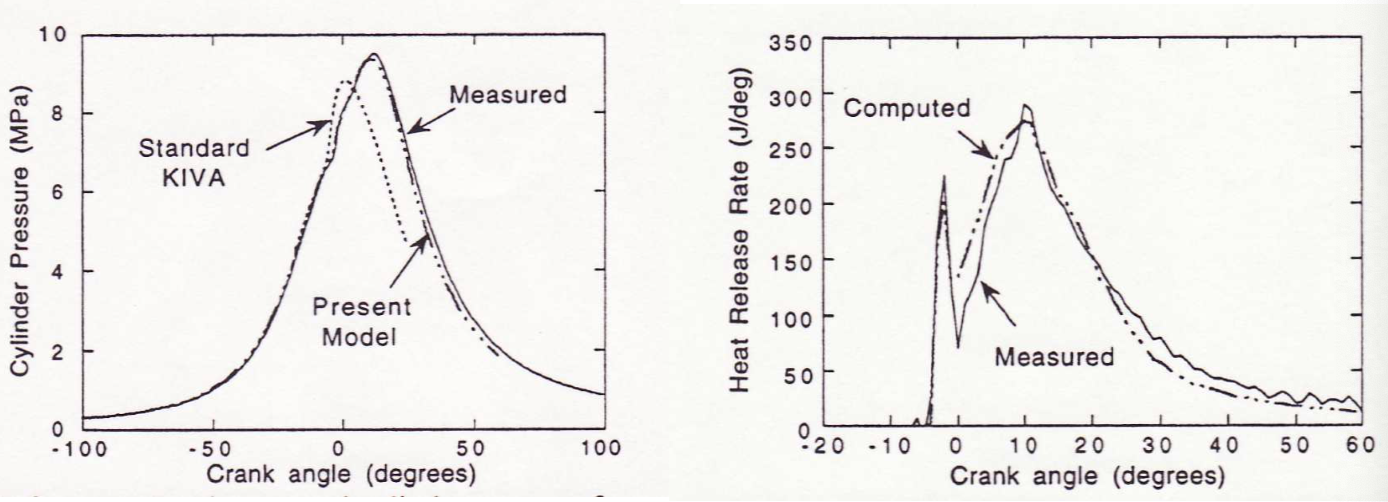
\includegraphics[width=0.6\textwidth]{figures/kiva.png}
\end{figure}

The figures show the computed and measured cylinder pressure (left) and the computed and measured heat release (right) for a Caterpillar engine.

\begin{figure}[!ht]
\centering
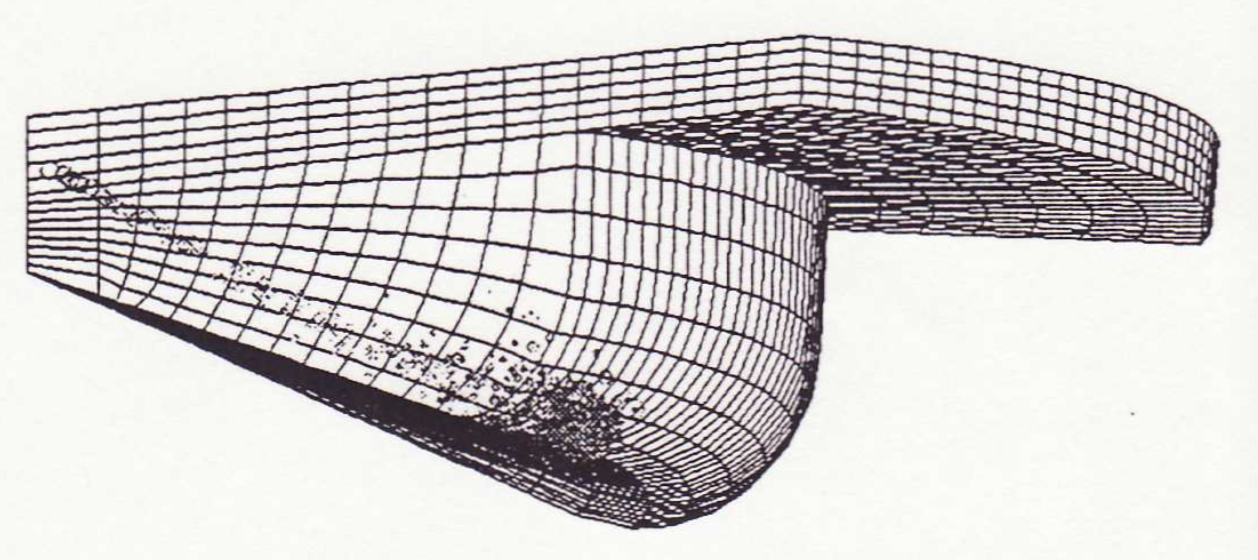
\includegraphics[width=0.4\textwidth]{figures/grid.png}
\end{figure}

Perspective view (1/6 of the combustion chamber) of the computational grid and fuel droplet distribution.

\begin{figure}[!ht]
\centering
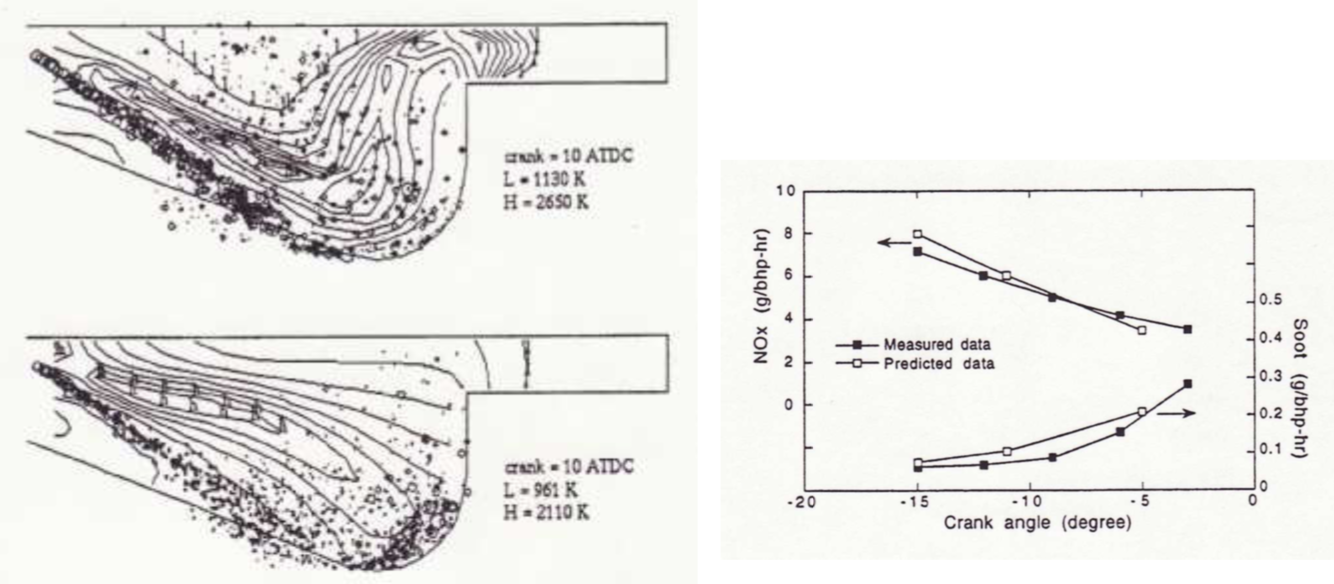
\includegraphics[width=0.6\textwidth]{figures/kiva2.png}
\end{figure}

In-cylinder gas temperature contours computed using different models (left), the wall impingement is visible. Comparison between computed emissions and measured engine-out data with varying fuel injection timing.

\begin{figure}[!ht]
\centering
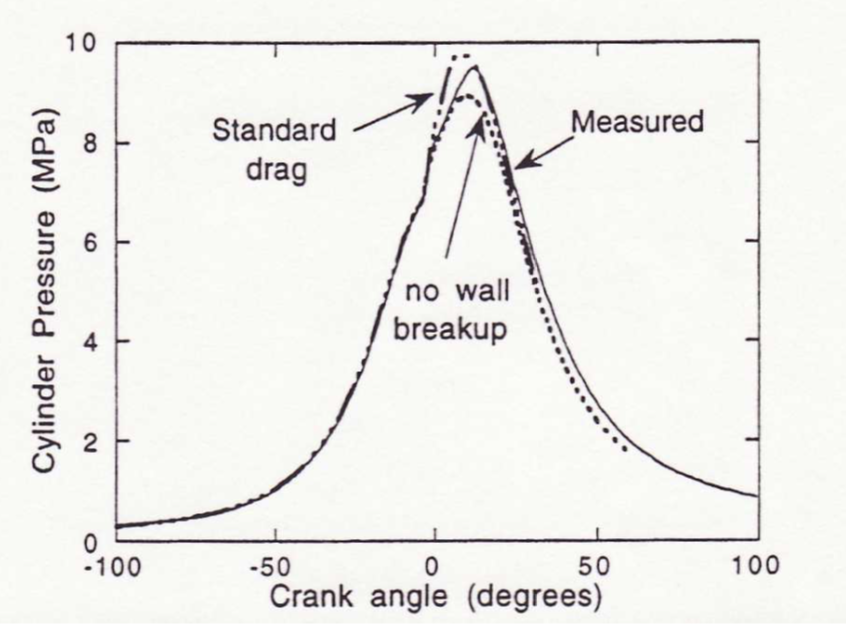
\includegraphics[width=0.5\textwidth]{figures/kiva3.png}
\end{figure}

Effects of drop drag and wall impingement on the combustion process.

\subsubsection{The spray model}

The spray model is a \textit{wave breakup model}, which take into account the wall impingement effects and drop drag varying coefficients. The fuel drop are injected with the size queal to the nozzle hole diameter and the number of drop is determined fromthe fuel flow rate. The mass of new droplets formed due to breakup is subtracted from the parent drop.\\
The high injection pressure in diesel engines produces a very high spray drop velocity with respect to the surrounfìding gas. Therefore the drop is subjected to high inertial forces which distort the drop into a disk shape. In order to model the trajectory of the drops, the drag coefficient must take into account this shape distortion since a distorted drop has a higher drag coefficient than a spherical drop.\\
Spray wall impingement is important since the impact of a drop on a heated surface may lead to its istantaneous vaporization or sliding and rebounding of a distorted drop (only the latter is modeled).

\subsubsection{The turbulence model}

The model is called \textit{RNG k-$\epsilon$}, an extra term is added to the dissipation equation which changes with the mean strain rate.
$k$ is the turbulent kinetic energy and $\epsilon$ is the dissipation rate:
\begin{equation}
    \frac{\partial \rho k}{\partial t}+\nabla\cdot(\rho u k)=...
\end{equation}
\begin{equation}
    \frac{\partial\rho\epsilon}{\partial t}+\nabla\cdot(\rho u \epsilon)=...
\end{equation}

\subsubsection{The ignition model}

A multistep kinetics model is adopted as the ignition model. The premise of the model is that \textit{degenerate branching} plays an important role in determining the cool flame and 2-stage ignition phenomena that are observed during the autoignition of hydrocarbon fuels.

\subsubsection{The combustion model}

This model is combind with the igniton model to simulate the overall combustion process in a diesel engine. The criterion to combine the ignition and combustion model is to switch between the models at $1000 K$. The igniton model is used when the temperature is lower than $1000 K$ to simulate the low temperature chemistry and viceversa. With this combustion model, the time rate of change of the partial density of species $m$ due to conversion from one chemical species to another, is given by:
\begin{equation}
    \frac{dY_{m}}{dt}=-\frac{Y_{m}-Y_{m}^{*}}{\tau_{c}}
\end{equation}
where $Y_{m}$ is the mass fraction of species $m$, $Y_{m}^{*}$ is the local equilibrium value of the mass fraction and $\tau_{c}$ is the characteristic time to achieve such equilibrium. An important aspect to this model is to formulate appropiately the characteristic time $\tau_{c}$ which is the sum of a laminar timescale and a turbulent timescale:
\begin{equation}
    \tau_{c}=\tau_{l}+f\tau_{t}
\end{equation}
where the \textit{delay coefficient $f$} determines the controlling role of turbulent effects.

\subsubsection{The emission model}

The extended \textit{Zel'dovich mechanism} is implemented to describe the $NO$ formartion. $NOx$ was found to be very sensitive to small changes in the computed gas temperature field. In order to obtain quantitative comparisons with experiments, a calibration factor $\beta$ is introduced:

\begin{equation}
    \bigg(\frac{dNO}{dt}\bigg)_{predicted}=\beta \bigg(\frac{dNO}{dt}\bigg)_{Zel'dovich}
\end{equation}

The soot emission model, written in the Arrhenius single step form, considers the rate of change of soot mass equal to the rate of formation less the rate of oxidation:

\begin{equation}
    \frac{dM_{soot}}{dt}= \frac{dM_{form}}{dt}- \frac{dM_{oxid}}{dt}
\end{equation}

\subsection{Spray generation}

Atomization is the process of conversion of the liquid fuel into small drops.\\ The aim is produce a high surface to mass ratio in the liquid phase in order to have a high evaporation rate. To this a high relative velocity between the liquid to be atomized and the sorrounding gas in needed which is what the \textit{pressure atomizers} and \textit{rotary atomizers} actually do. The \textit{airblast atomizers} instead eject a high velocity airstream on a slow liquid film. The Weber number provide a usel indication of both the quality and the nature of the atomization process.

\subsubsection{Spray characteristics}

\begin{itemize}
    \item \textit{Mean drop size}: the idea is to replace a given spray with one in which the droplets have the same diameter, retaining the characteristics of the original spray.
    \item \textit{Drop size distribution}: drop sizes range in diameter from $10$ to $400 \mu m$.
    \item  \textit{Patternation}: the uniformity of the circumferentual distribution of fuel in a conical spray. Poor patternation affects pollutants emission.
    \item \textit{Cone angle}: if the cone angle is narrow, drops are evenly dispersed through the entire spray (\textit{solid spray}). With swirl atomizers, a hollow conical structure of the spray is obtained allowing a better exposure to the sorrounding air.
    \item \textit{Dispersion}: the ratio of the volume of the spray to the volume of the fuel contained with it. A good dispersion allows a good mixing of the fuel with the surrounding gas, with an increase in the evaporation rate and heat release.
    \item \textit{Penetration}: maximum distance the spray reaches when injected in stagnant air. It is governed by the kinetic energy and the aerodynamic resistance. Compact narrow spray has high penetration. The penetration of a spray is greater than that of a single drop since the gas offers less resistance to the following drops which penetrate further.
\end{itemize}

\subsubsection{Simplex atomizer}

\begin{figure}[!ht]
\centering
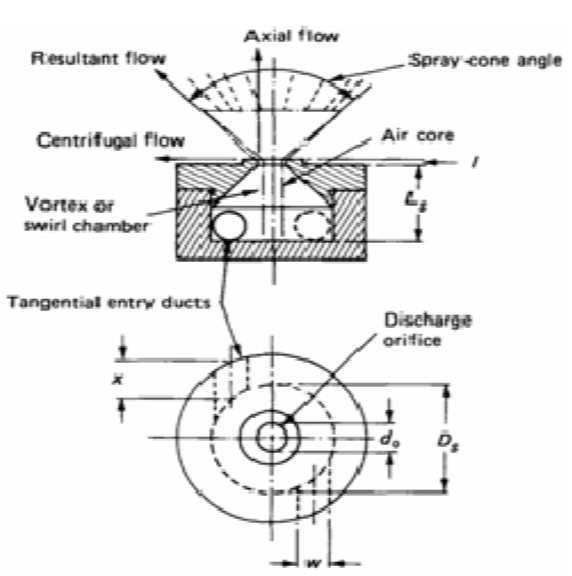
\includegraphics[width=0.5\textwidth]{figures/simplex.png}
\end{figure}

It is a pressure-swirl atomizer. The fuel is fed into a swirl chamber through tangential ports that give the fuel a high angular velocity. The rotating fluid flows through the orifice in the form of a hollo conical sheet. As the air pressure increases, the size distribution is shifted toward smaller drop diameters. The major drawback is that the flow rate varies as the square root of the pressure differential. Therefore, doubling the fuel flow rate requerise fourfold increase in pressure.

\subsubsection{Duplex atomizer}

The drawback of the simplex atomizer has led to the development of wide range atomizers such as \textit{duplex}, \textit{dual orifice} and \textit{spill} atomizers.

\begin{figure}[!ht]
\centering
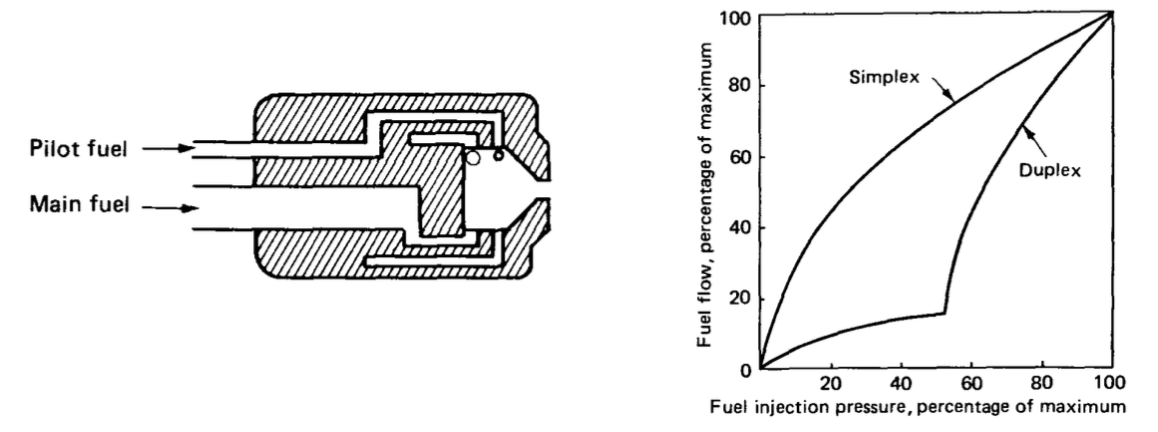
\includegraphics[width=0.8\textwidth]{figures/duplex.png}
\end{figure}

Two simplex nozzles are fitted concentrically, one inside the other. At low fuel flow all the fuel is supplied from the pilot nozzle, when the fuel pressure reaches a fixed value, the pressurising valve opens and admits fuel to the main nozzle.

\begin{figure}[!ht]
\centering
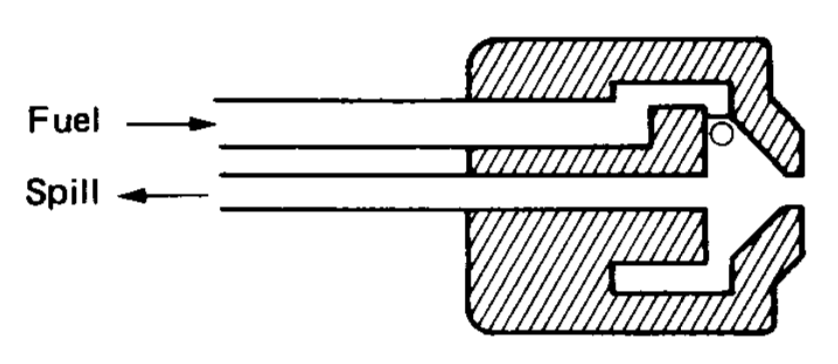
\includegraphics[width=0.5\textwidth]{figures/spill.png}
\end{figure}

The spill atomizer is a simplex atomizer but with a passage through which fuel can be spilled away from the atomizer. There is a constant use of a high pressure meaning that at low fuel flows the swirl is adequate to provide an efficient atomization of the fuel.
//In the rotary atomizer the fuel is fed into a rotating surface where it spreads out under the action of centrifugal force.

\begin{figure}[!ht]
\centering
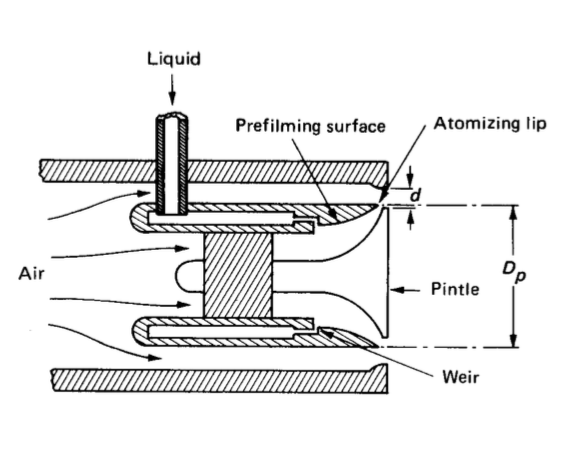
\includegraphics[width=0.5\textwidth]{figures/airblast.png}
\end{figure}

The airblast atomizer improve the atomization by prefilming the fuel and introducing air at high speed.

\newpage

\section{Reacting boundary layer}

A boundary layer is defined as the flow region of moving fluid in qhich shear stresses, heat fluxes and mass diffusion fluxes are significant only in the direction normal to the direction of flow (they don't require the presence of solid walls).Chemical reaction can develop in a geseous phase or in form of heterogeneous reactions at the surface.
The boundary layer flow can be laminar or turbulent, stationary or nonstationary, single-phase or multiphase. The free current flow may be subsonic, transonic, supersonic or hypersonic.

\subsection{The governing equations}

The governing partial differential equations for chemically reacting boundary layers are derived from conservation equations. Order of magnitude analysis is used for the simplification of equations (5 + N variables).\\
The thickness of the boundary layer is assumed to be much smaller than the plate length ($x/L<<1$) and the approximation states:
\begin{equation}
    \frac{\partial u}{\partial x} ~ \frac{u}{L}
\end{equation}

\begin{equation}
    \frac{\partial u}{\partial y} ~ \frac{u}{\delta}
\end{equation}

The continuity equation and the momentum equation for the steady 2-dimensional boundary layer are written as:

\begin{equation}
    \frac{\partial (\rho u)}{\partial x} + \frac{\partial (\rho v)}{\partial y} = 0
\end{equation}

\begin{equation}
    u \frac{\partial u}{\partial x} +  v \frac{\partial u}{\partial y} = - \frac{1}{\rho}\frac{\partial p}{\partial x} + \frac{1}{\rho} \frac{\partial}{\partial y}\bigg( \mu \frac{\partial u}{\partial y} \bigg)
\end{equation}

The dimplified balance equation for the \textit{ith} species can be written as:

\begin{equation}
    \rho \bigg(u \frac{\partial Y_{i}}{\partial x} +  v \frac{\partial Y_{i}}{\partial y} \bigg) - \frac{\partial}{\partial y} \bigg( \rho \mathcal{D_{i}} \frac{\partial Y_{i}}{\partial y} \bigg) = \omega_{i}
\end{equation}

If the body force and radiation is neglected, the nergy equation in terms of enthalpy becomes:

\begin{equation}
    \rho \bigg(u \frac{\partial h}{\partial x} +  v \frac{\partial h}{\partial y} \bigg) = u \frac{\partial p}{\partial x} - \frac{\partial q_{y}}{\partial y} + \mu \bigg(\frac{\partial u}{\partial y} \bigg)^{2}
\end{equation}

where enthalpy includes the chemical energy

\begin{equation}
    h = \sum_{i=1}^{N} Y_{i}h{i}
\end{equation}
and
\begin{equation}
    h_{i} = \int_{T_{0}}^{T} C_{p,i}dT + \Delta h_{f,i}^{0}
\end{equation}

\subsection{The model for the reacting turbulent boundary layer}

In the following set of equations for the axisymmetric flows $m=1$, whereas fot planar flows $m=0$ and the variable $r$ is replaced by $y$.

\begin{figure}[!ht]
\centering
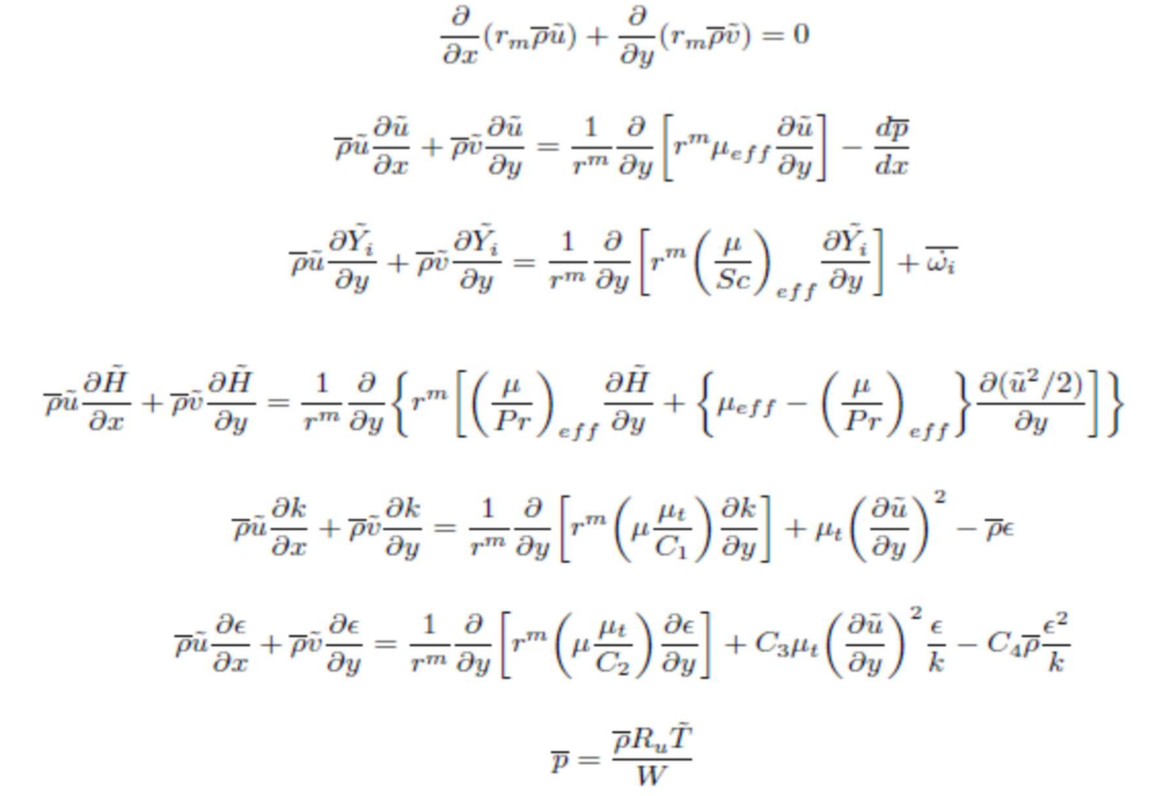
\includegraphics[width=0.8\textwidth]{figures/turbulent.png}
\end{figure}

\subsection{Governing equations for the inviscid region}

For the potential flow regionsm assuming a planar flow at freestream boundary, the following system of equations are considered:

\begin{equation}
    \Tilde{u} = U_{\infty}, \;\;\; \Tilde{T}=T_{\infty}
\end{equation}
\begin{equation}
    \frac{\partial \Tilde{Y}_{F}}{\partial y} =  \frac{\partial \Tilde{Y}_{0}}{\partial y} = 0
\end{equation}
\begin{equation}
    \frac{\partial k}{\partial y} = \frac{\partial \epsilon}{\partial y} = 0
\end{equation}

\subsection{Modeling of the gas-phase chemical reactions}

The term $\dot{omega}$ must be known in order to solve the system of equations with appropiate boundary conditions. In the following, a reacting turbulent boundary layer flow is considered over solid fuel. The chemical reactions of the pyrolysed gaseous reactants emitted by the solid surface are translated into a single irreversible chemical reaction:

\begin{equation}
    v_{F}F + v_{o}O \rightarrow v_{P}P
\end{equation}

Using the Arrhenius law implies some difficulties in the time averaging of the resulting exponential expression. This suggest an alternative approach know as \textit{eddy-breakup model} (EBU). From such a model, the following expression for $\dot{\omega}_{F}$ is obtained:

\begin{equation}
    \dot{\omega}_{F} = -C_{\dot{\omega}}\rho \sqrt{k} \bigg| \frac{\partial \Tilde{Y}_{F}}{\partial r}\bigg|
\end{equation}

where $C_{\dot{\omega}}$ is a constant.

\newpage

\section{Supersonic combustion and detonation}

In the study of detonation attention will be concentrated on the premixed flame. Reactions of the premixed gases are generally divided into three categories:

\begin{itemize}
    \item \textit{explosion}: the rate of heat generation is extremely fast, but it does not require the passage of a combustion wave through the exploding mixture
    \item \textit{deflagration}: the combustion wave propagates at subsonic speed
    \item \textit{detonation}: the combustion wave propagates at supersonic speed
\end{itemize}

Flames in combustibile gas mixture in tubes reaches enourmous velocities (~$3500 m/s$). Detonation waves are shock waves which are sustained by the energy of the chemical reaction that is initiated by the shock compression. Their rate of propagation is limited by the rate at which a shock wave can travel.

\subsection{Shock wave in a neutral gas}

Consider a long tube closed at the left by a piston. A small velocity $dw$ is imparted to the piston, this movement produces in the gas a weak compression wave that travels from left to roght with the velocity of sound. The gas to the right of the wave front is at rest, while the gas between the wave front and the piston is compressed adiabatically by $dp$ and has the velocity $dw$. Then, the velocity of the piston is increased by another $dw$, a second compression wave is produced in the gas. By ripetition of this procedure the velocity of the piston is brought to the final velocity $w$.

\begin{figure}[!ht]
\centering
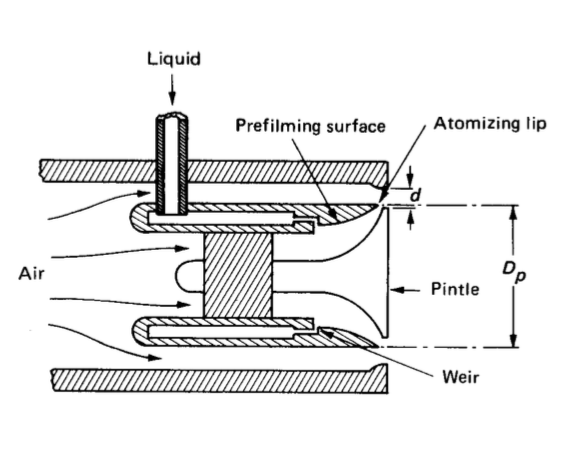
\includegraphics[width=0.5\textwidth]{figures/airblast.png}
\end{figure}

A step-like set of waves is produced. The upper steps of the terrace have greater velocity than the lower steps since the temperature and theredore the velocity of sound is larger in the gas in the upper steps. As soon as the steps are merged, a shock wave with very high steep pressure gradient is formed. After the piston has attained its constant velocity $w$, the column of gas is pushed ahead at the same velocity $w$. Work must constantly be performed by the piston in order to mantain the motion.\\
Consider a coordinate system moving with the wave front. Since the process is stationary, the masses, momenta and energies are constant:

\begin{equation}
    \frac{u_{1}}{v_{1}} =  \frac{u_{2}}{v_{2}}
\end{equation}

\begin{equation}
    \frac{u_{1}^{2}}{v_{1}} + p_{1} =  \frac{u_{2}^{2}}{v_{2}} + p_{2}
\end{equation}

\begin{equation}
    E_{1} + \frac{u_{1}^{2}}{2} + p_{1}v_{1} = E_{2} + \frac{u_{2}^{2}}{2} + p_{2}v_{2}
\end{equation}

The equations represent the conservation of mass, momentum and energy.\\
The velocity of propagation $D$ of the shock wave into the gas at rest is found to be:

\begin{equation}
    D = u_{1} = v_{1}\sqrt{\frac{p_{2}-p_{1}}{v_{1}-v_{2}}}
\end{equation}

and the velocity $w$ of the gas behind the wave (particle velocity) is

\begin{equation}
    w=u_{1}-u_{2}= (v_{1}-v_{2})\sqrt{\frac{p_{2}-p_{1}}{v_{1}-v_{2}}}
\end{equation}

\subsection{The detonation wave}

We now consider a shock wave traveling in combustible gas. Plane $1$ lies in the unburned gas and plane $2$ in the burned gas. The previous set of equation are valid, however the energy difference represent only the change in internal energy caused by compression, whereas now the temperature of the gas passing through plane 2 has been increased due to energy $\Delta E_{c}$ in the reaction:

\begin{equation}
    \Delta E = C_{v}(T_{2}-T{1}) - \Delta E_{c}
\end{equation}

\subsection{The Rankine-Hugoniot curve}

\begin{figure}[!ht]
\centering
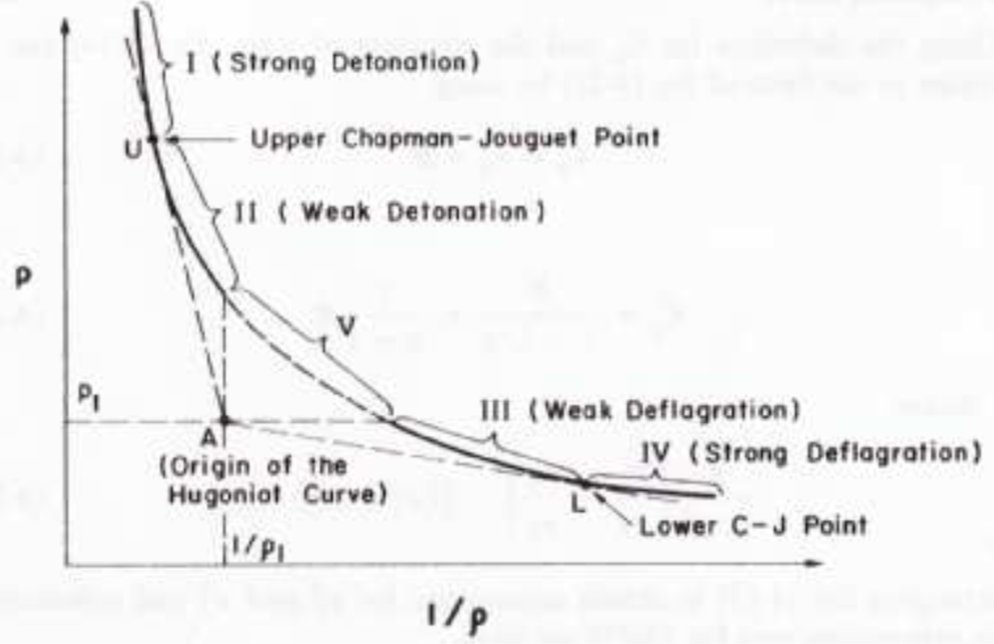
\includegraphics[width=0.5\textwidth]{figures/rankine.png}
\end{figure}

It is essentialy a plot of all possible valies of $1/\rho_{2}$ and $p_{2}$ for a given value of $1/\rho_{2}$, $p_{2}$ and $q$. The point $1/\rho_{2}$ is called the origin. Regions of possible solutions are constructed by drawing tangents to the curve through the point A, and the curve is divided into five regions. The two tangent points to the curve are called \textit{C-J points}. It must be noted that although the curve represents all the possible solutions of the Hugonoit equation (energy eq.), not all the solutions are valid since in the region V the line implies that $u$ is imaginary (physically impossible region).

\subsection{Deflagration detonation comparison}

\begin{figure}[!ht]
\centering
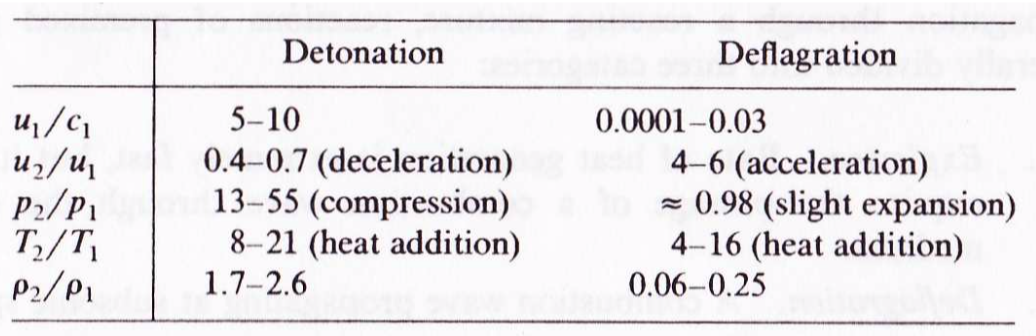
\includegraphics[width=0.5\textwidth]{figures/defla.png}
\end{figure}

All the possible values to compute the equations are found in tables, including the limits of detonability (in per cent fuel).

\newpage

\section{Fuels and propellants}

Hydrocarbons are obtained by oil distillation. Oil is a complex mixture of gas, liquids and solid substances which mainly consists of hydrocarbons, nitrogen, sulphur organic compounds and small quantities of metal constituents. Pure hydrocarbons are composed of only two elements, carbon $C$ and hydrogen $H$. At ambient temperature they can be in gaseous, liquid or solid form, depending on the number of carbon atoms and on the molecular structure. Hydrocarbons up to 4 carbon atoms are gaseous, with 20 ore more carbon atoms are solid, in between are liquid.

\subsection{Fuels}

It is usual to classify hydrocarbons inthe following 5 series:

\begin{itemize}
    \item \textit{Alkanes (paraffins)} $[C_{n}H_{2n+2}]$: the symples hydrocarbon, \textit{methane}, belongs to this series. Hydrocarbons for aeronautical use contain from 35 to 45\% of paraffins. Paraffins have a high ratio hydrogen/carbon, a low density, a high heat of combustion and their combustion is characterized by low carbon deposits and low smoke production. In reciprocating combustion engines they show a low resistance to knock (ability not to self-ignite and burn in an uncontrolled way while the fuel is being compressed).

\begin{figure}[!ht]
\centering
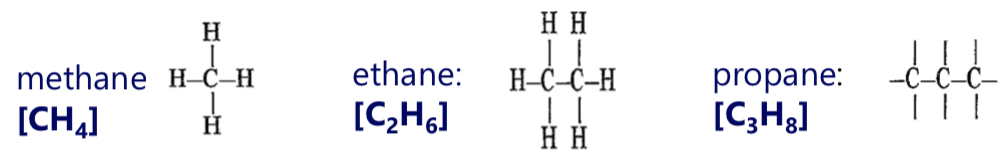
\includegraphics[width=0.5\textwidth]{figures/paraffins.png}
\end{figure}

    \item \textit{Alkanes (olefins)} $[C_{n}H_{2n}]$: olefins do not exist in oil. They come from refining processes. Their molecules contain a lower number of hydrogen atoms, compared to the maximum possible value. Olefins are very active a quickly react with many compounds to form rubbers. For this reason they are undesired in the fuels for gas turbines. The lightest molecule of this series is \textit{ethylene} $(C_{2}H_{4})$ which contains a double bond between the carbon atoms.

\begin{figure}[!ht]
\centering
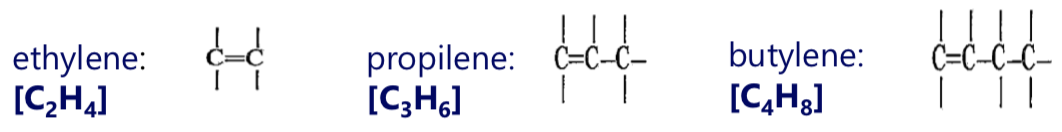
\includegraphics[width=0.5\textwidth]{figures/olefins.png}
\end{figure}

    \item \textit{Alkynes (acetylene series)} $[C_{n}H_{2n-2}]$: they are unsaturated hydricarbons which contain a triple bond. The first member od the series is \textit{acetylene} $C_{2}H_{2}$, very unstable. They have a high combustion temperature and a high flame speed.
    \item \textit{Cyclanes (naphthenes)} $[C_{n}H_{2n}]$: saturated hydrocarbons, in which carbon atoms form rings instead of chains. In distelled fuels they are in the same proportion of paraffins (35 to 45\%). Similar to paraffins for chemical stability, heat combustion, and the low tendency to produce smoke.

\begin{figure}[!ht]
\centering
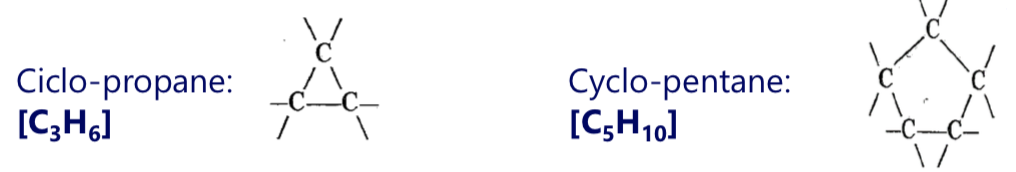
\includegraphics[width=0.5\textwidth]{figures/cyclanes.png}
\end{figure}

    \item \textit{Aromatics} $[C_{n}H_{2n-6}]$: the molecular structure is a ring, with six carbon atoms and three double bonds. They contain a lower amount of hydrogen and consequently their heat of combustion is lower. Another disadvantage is the high smoke production and high hygroscopicity, which can lead to crystals precipitation when the fuel is at low temperature. Aromatics have a high solvent activity in the rubbers, this can lead to serious problems during fuel feeding in aircrafts with rubber tanks. The simplest aromatic is $benzene$.

\begin{figure}[!ht]
\centering
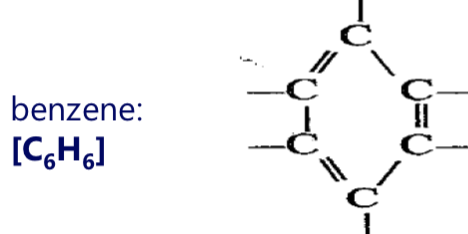
\includegraphics[width=0.2\textwidth]{figures/aromatics.png}
\end{figure}

\end{itemize}

\subsection{Fuel properties}

\begin{itemize}
    \item \textit{Relative density}: ratio between the mass of a given amount of fuel at temperature $T_{1}$ and the mass of the same volume of pure water at temperature $T_{2}$. Typical values are in the interval of 0.72 to 0.97.
    \item \textit{Interval of distillation}: it affectes the physical characteristics of the fuel.
    \item \textit{Vapor pressure}: it is the pressure of vapor on the liquid surface at a certain temperature. A high vapor pressure is desired due to the rapid evaporation in the primary zone. Low vapor pressure imply lower losses due to the fuel evaporation at high altitudes.
    \item \textit{Flash point}: it is defined as the lowest temperature at which a fuel develops enough vapor to form an ignitable mixture with the surrounding air. Higher is the vapor pressure, lower is the flash point.
    \item \textit{Volatility}: if high, easier ignition, better stability, higher combustion efficiency. Disadvantages are evaporation losses at high altitude.
    \item \textit{Viscosity}: important for the atomization process, depends on temperature.
    \item \textit{Freezing point}: freezing points are at $227 K$ or $215 K$ depending on the type of service.
    \item \textit{Specific heat}: it is important for cooling of the aircraft structure at high Mach number. Paraffins are the best fuels since they have the highest specific heat.
\end{itemize}

Three liquid bipropellant combinations are commonly used today:

\begin{itemize}
    \item \textit{cryogenic oxygen-hydrogen} propellant system, used in upper stages of space lunch vehicles, it gives the highest specific impulse for non-toxic combination
    \item \textit{liquid oxygen-hydrocarbon} propellant combination, used for booster stages of space launch vehicles, its higher average density allows a more compact booster stage
    \item \textit{storable propellant combinations} used in large rocket engines for first and second stage
\end{itemize}

\subsection{Propellants performance}

The performance can be compared on the basis of the specific impulse, the specific propellant consumption and the effective or ideal exhaust velocity. For high performance a high content of chemical energy per unit of propellant mixture is desirable because it permits high chamber temperature. A low molecular mass of product gasses ia also desirable, it is accomplished if a large portion of the hydrogen produced does not combine with oxygen. In general, therefore the best mixture ratio for many bipropellants is not the stoichiometric one but usually a fuel-rich mixture containing a large portion of low-molecular-mass products.

\subsection{Common physical hazards}

\begin{itemize}
    \item \textit{Corrosion}: various propellants have to be handled in containers and pipelines of special materials.
    \item \textit{Explosion hazard}: some propellants are unstable and tend to detonate under certain conditions of impurities, temperature and shock.
    \item \textit{Fire hazard}: many oxidizers will start chemical reactions spontaneously with many organic substances. Most fuels are readily ignitable when exposed to air and heat.
    \item \textit{Health hazards}: many propellants are toxic or poisonous and special precautions have to be taken to protect personnel.
\end{itemize}

\subsection{Desirable physical properties}

\begin{itemize}
    \item \textit{Low freezing point}
    \item \textit{HIgh specific gravity}: in order to accomodate a large mass of propellants in a tank, high density is required.
    \item \textit{Stability}: no decomposition of the liquid propellant during operation or storage. Minimal reaction with the atmosphere.
    \item \textit{Heat transfer properties}: high specific heat, high thermal conductivity, high boiling temperature.
    \item \textit{Pumping properties}: a low vapor pressure permits a more effectuve pump design reducing the potential for cavitation. If the viscosity is too high the design become difficult.
    \item \textit{Ignition}: spontaneously ignitable propellants (hypergolic) means that burning is initiated as the oxidizer and the fuel come in contact. If autoignitable it does not require an ignition system.
    \item \textit{No variations}: properties must now vary, because this can affect engone performance.
    \item \textit{Additives}: tailoring propellant properties can be achieved with additives.
\end{itemize}

\subsection{Liquid oxidizers}

\begin{itemize}
    \item \textit{Liquid Oxygen} $O_{2}$: boils at $90 K$ at atmospheric pressure. It is widely used as an oxidizer and burns with most hydrocarbon fuels. Because liquid oxygen evaporates rapidly, it cannot be stored readily for long time so it is produced very close to its application. It is necessary to insulate all lines and tanks in order to reduce the evaporation loss.
    \item \textit{Hydrogen Peroxide} $H_{2}O_{2}$: in rocket applications is used in a highly concentrated form (70 to 99\%), the remainder is water. The theoretical specific. Even under favorable conditions it decomposes at a slow rate during storage.
    \item \textit{Nitric Acid} $HNO_{3}$: there are several types of nitric acid mixtures that have been used as oxidizers but they are not used extensively today. The most common are the \textit{red duming nitric acid} and the \textit{white duming nitric acid}. Nitric acid is highly corrosive. The high density permits compact storage.
    \item \textit{Nitrogen Tetroxide} $N_{2}O_{4}$: this is a high-density yellow liquid. Although it is the most common storable oxidizer used, its liquid temperature range is narrow and it is easily frozen or vaporized. It is hypergolic with many fuels and can cause spontaneous ignition. The fumes are brown and are extremely toxic. Its properties make it a very good oxidizer for space applications.
\end{itemize}

\subsection{Liquid fuels}

\begin{itemize}
    \item \textit{Hydrocarbon Fuels}: petroleum derivatives such as gasoline, kerosene, diesel oil and turbojet fuel. Their properties vary with the type of crude oil from which they were defined and with the chemical process used in their production.
    \item \textit{Liquid Hydrogen} $H_{2}$: when burned with liquid fluorine or liquid oxygen it gives a high performance. It also is an excellent coolant. It burns with a colorless flame. Of all known fuels, liquid hydrogen is the lightest and the coldest. Its very low fuel density requires big tanks and the extremely low temperature makes the problem of choosing suitable tank difficult since many metals become brittle at low temperatures.
    \item \textit{Hydrazine} $N_{2}H_{4}$: is used as bipropellant fuel as well as monopropellant. It is a toxic colorless liquid with a high freezing point. Hydrazine has a short ignition delay and is spontaneously ignitable with nitric acid, nitrogen tetroxide and also air. Pure hydrazine is stable and can be stored in sealed tanks for over 15 years. With impurities it decomposes so tanks and pipes must be cleaned of impurities.
    \item \textit{Unsymmetrical Dimethylhydrazine} $(CH_{3})_{2}NNH_{2})$: a derivative of hydrazine, is often used in mixtures with hydrazine since it forms a more stable liquid. It has lower freezing point.
    \item \textit{Monomethylhydrazine} $(CH_{3}NHNH_{2})$: has been used as a fuel in small attitude control engines. It has better heat transfer and better liquid temperature range than pure hydrazine. All hydrazines are toxic materials but this one is the most of them.
\end{itemize}

\subsection{Liquid monopropellants}

\begin{itemize}
    \item \textit{Hydrazine} as a monopropellant: hydrazine is not only an excellent storable fuel, but also an excellent monopropellant when decomposed by a suitable catalyst.
    \item \textit{Hydroxyl Ammonium Nitrate}: this is a new synthetic propellant material rich in oxygen. The liqyid us corrosive, toxic, denser than hydrazine monopropellant.
\end{itemize}

\subsection{Gaseous propellants}

Cold gas propellants have been used for many years. The engine consists of one or more high-pressure gas tanks, multiple metal nozzles, an electrical control valve with each nozzle. The tank size is smaller if the tank pressures are high.

\subsection{Solid propellants}

There are 2 classes:

\begin{enumerate}
    \item \textit{Double-base (DB) propellants}: form a homogeneous propellant grain with a minor percentage of additives.
    \item \textit{Composite propellants}: form a heterogeneous propellant grain with the oxidizer crystals and a powdered fuel held together by a binder.
\end{enumerate}

\subsubsection{Propellant characteristics}

\begin{itemize}
    \item High performance or high specific impulse, this meand high temperature or low molecular mass.
    \item Predictable burning rate to fit the need of grain design.
    \item High density.
    \item Good aging characteristics and long life.
    \item Low absorption of moisture, which causes chemical deterioration.
    \item Simple manufacturing. Non-toxic exhaust gases.
    \item Not prone to combustion instability.
\end{itemize}

\begin{figure}[!ht]
\centering
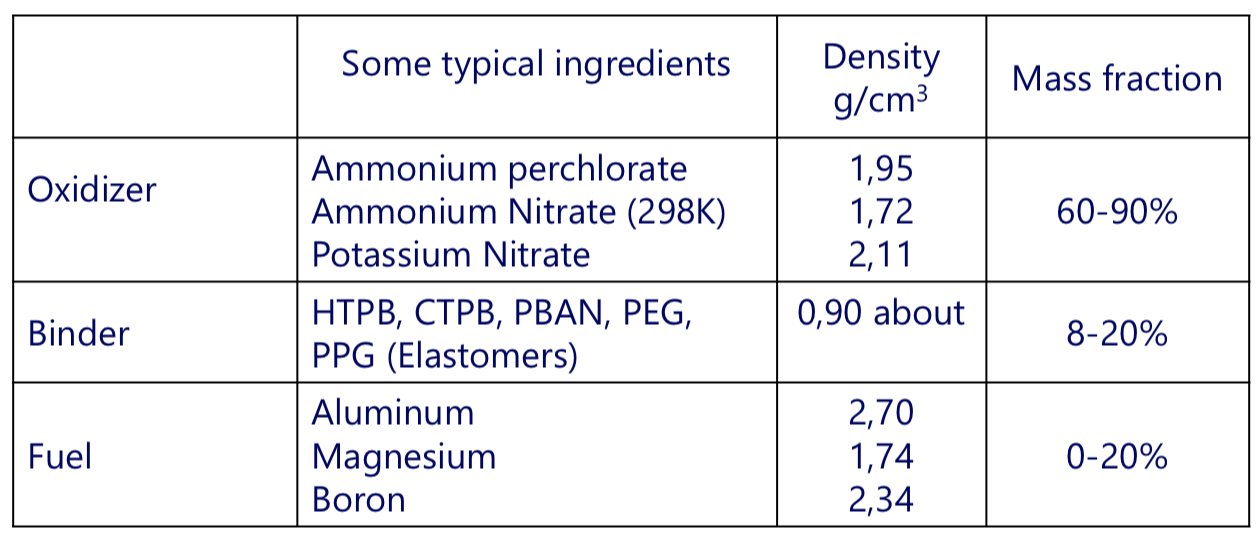
\includegraphics[width=0.5\textwidth]{figures/table.png}
\end{figure}

\subsubsection{Manufactring}

The solid ingredients (powder and oxidizer) are mixed in the pre-polymer, along with plasticizers and curing agents. The highly viscous compound is cast in forming molds. Then, the propellants is solidified.
\begin{itemize}
    \item \textit{Debonding of interfaces}: detachment between propellant and thermal protection. The flame propagates inside the opening.
    \item \textit{Dewetting (cohesive fracture)}: in some regions, the contact between binder and particles is lost. Vaculoes are opened. When loaded, cracks open and propagate.
\end{itemize}

\subsubsection{The oxidizer}

The typical oxidizer is the ammonium perchlorate which is an inorganic salt, non-toxic and soluble in water. Products of the combustion include cloridric acif ($HCl$) and other substances highly toxic and corrosive.

\subsubsection{The polymeric binder}

Its role is the coesion of cristallin ingredients and it is responsible for elasticity and mechanical properties. It is also the fuel, responsible for a regular and complete combustion. Typically, propellants have a binder mass fraction between 14\% and 17\%. If low the mixture is more reactive, if high incomplete combustion.

\subsubsection{Metal powders}

Oxidation of $Al$ to $Al_{2}O_{3}$ is strongly exothermic and it has higher density compared to other propellants ingredients. It has combustion products with a lower molecular weight and it improves the specific impulses.\\
Cons:
\begin{itemize}
    \item higher temperature means higher thermal stresses and heavier thermal protections
    \item generation of metal agglomerates which cause a reduction of the specific impulse. Coarse fraction of agglomerates is removed by the use of nanoaluminum.
\end{itemize}

\subsection{Green propellants}

\textit{Ammonium perchlorate} (AP) and \textit{hydrazine} are today used as propellants. AP as oxidizer in solid propellants and hydrazine as liquid monopropellant. These propellants are well known for their good performance characteristics, but their limitations regarding toxicity, operational handling and environmental impact are also well documented (bad).\\
Propellants of the future must not present hazards to the crew or personnel. The use of green propellants would reduce the risks associated with toxicity, operational handling complexity, spacecraft contamination, and contamination of the environment. Green propellants have also shown promise from performance and total life cycle cost perspective.\\
One material that has the potential to replace AP as well as hydrazine is \textit{ammonium dinitramide} (ADN). It is a solid white salt, work is in progress on improving the mechanical properties, to characterize the sensitivity, on ignition and thruster development.

\newpage

\section{Environmental impact of combustion processes}

Pollutants from gas turbines:
\begin{itemize}
    \item $CO$: carbon monoxide (extrmely toxic)
    \item $UHC$: Unburnt Hydro Carbon (mutagenic effects)
    \item $NO_{x}$: nitrogen oxides (affect the ozone belt)
    \item $SO_{x}$: sulphur oxides (acid rains)
    \item $CO_{2}$ and $H_{2}O$: not pollutants but responsible of greenhouse effect
\end{itemize}

The most interesting and important pollutant is $NO_{x}$ with the linked reactions with ozone:
\begin{equation}
    NO+O_{3} \rightarrow NO_{2}+O_{2}
\end{equation}
\begin{equation}
    NO_{2}+O \rightarrow NO+O_{2}
\end{equation}

the first equation shows the depletion of ozone, the second as nitric oxide ($NO$) is produced to react again (loop).

\subsection{Carbon monoxide}

High $CO$ concentration due to rich mixtures in the primary zone and due to poor oxygen concentration for the oxidation of $CO$ to $CO_{2}$. It is possible to reduce this concentration to negligible values introducing air after the primary zone to abtain a progressive reduction of combustion products temperature.\\
Mainly $CO$ comes from the incomplete combustion of the fuel. This is caused by:
\begin{itemize}
    \item not good reaction rates in the primary zone, due to a too low mixture ratio or insufficient residence time
    \item not good mixing
    \item extinction of combustion due to cooling air
\end{itemize}

Low $CO$ levels can be obtained in a narrow interval of equivalence ratios (between 0.7 and 0.9). Since for lower $\phi$, $CO$ levels are high due to low oxidation rate, for higher $\phi$, $CO$ levels are high due to equilibrium.\\
At low temperature the main reaction of $CO$ removal is:
\begin{equation}
    CO+H_{2}O \leftrightarrow CO_{2}+H_{2}
\end{equation}
At high temperature the main reaction of $CO$ removal is:
\begin{equation}
    CO+OH \leftrightarrow CO_{2}+H
\end{equation}

\subsection{Unburnt hydrocarbons}

They include fuel, not completely oxidized, which leaves the combustion chamber in form of vapor or droplets, as well as thermal degradation products at lower molecular weight, such as methane or acetylene. They are dye to poor mixing, low chemical reaction rates or effects due to the cooling air. Increases in the engine power reduce the emission of the unburnt hydrocarbons, due to increase of the chemical reaction rates in the primary zone.

\subsection{Nitrogen oxides}

Nitrogen oxides are products of the atmospheric nitrogen oxidation in the regions of high temperature of the flame. The process in endothermic, $NO$ develops only in the central regions of the combustion chamber at the highest temperature.\\
It is produced through 3 mechanisms:
\begin{itemize}
    \item $NO$ thermal: oxidation in the post-flame gases
    \item $NO$ prompt: generated at the flame front through fast reactions
    \item $NO$ of the fuel: due to oxidation of nitrogen contained in fuel
\end{itemize}

The first is the most significant mechanism. $NO$ thermal is produce through the Zeldovich mechanism:
\begin{equation}
    O_{2} \leftrightarrow 2O
\end{equation}
\begin{equation}
    O + N_{2} \leftrightarrow NO + N
\end{equation}
\begin{equation}
    N + O_{2} \leftrightarrow NO + O
\end{equation}

\begin{figure}[!ht]
\centering
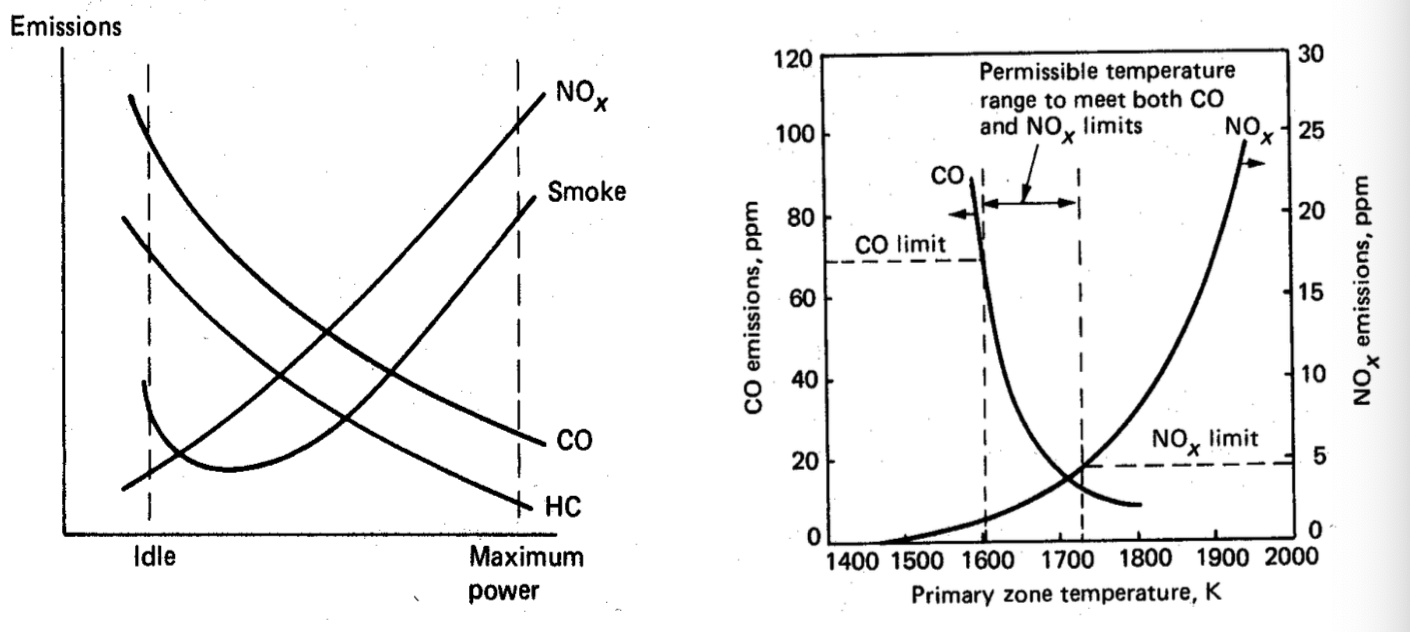
\includegraphics[width=0.8\textwidth]{figures/pollutants.png}
\end{figure}

\newpage

\section{Combustion in air-breathing engines: gas turbines}

The design of a combustion chamber aims to reduce the size of the chamber, completing all the processes occuring:
\begin{itemize}
    \item injection of the liquid
    \item fuel atomization
    \item fuel vaporization
    \item mixing of fuel vapor with the air
    \item development and completion of chemical reactions
\end{itemize}
In order to keep the engine size small, the intensity of combustion is usually very high 500000 $KJ/(m^{3}s))$.

\begin{figure}[!ht]
\centering
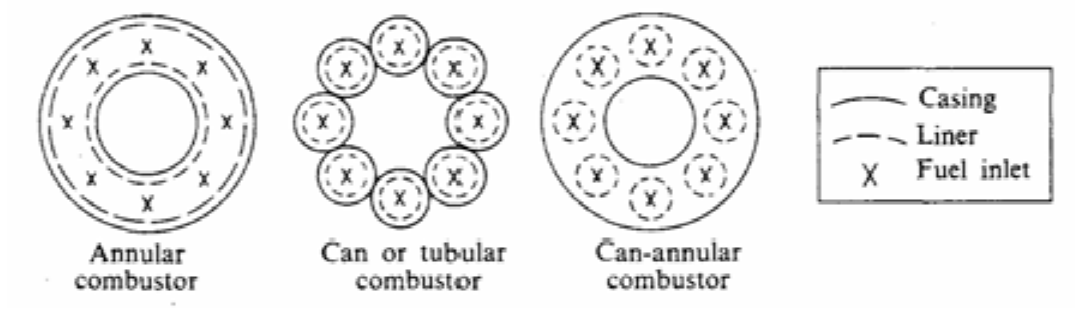
\includegraphics[width=0.7\textwidth]{figures/gaschamber.png}
\end{figure}

Chemical reactions are confined to the interior of a perforated liner . The air flow moving between the liner and the casing keeps the metal cool enough to mantain its mechanical properties.\\
High turbulence is needed for intense combustion. This causes a considerable pressure drop.

\subsection{Approximate calculation of mixture ratio}

\begin{figure}[!ht]
\centering
\includegraphics[width=0.5\textwidth]{figures/mixturetable.png}
\end{figure}

Approaching the turbojet combustion as a heating process, we can write:
\begin{equation}
    \dot{m}_{f}\Delta H_{r} = \dot{m}_{a}C_{p}(T_{04}-T_{03}) \rightarrow f = \frac{\dot{m}_{f}}{\dot{m}_{a}} = \frac{C_{p}(T_{04}-T_{03})}{\Delta H_{r}}
\end{equation}
Normal value of the mixture ratio (0.025) are lower than the respective stoichiometric ratio. This is due to prevent the high temperature at the exit of the combustion chamber.\\
The required value of f would lead to a mixture too lean for ignition and combustion. For this reasin the fuel, is initially mixed and burned with a small amount of primary air.

\begin{figure}[!ht]
\centering
\includegraphics[width=0.6\textwidth]{figures/airdistribution.png}
\end{figure}

The primary zone is fed by ~20\% of the airflow, about 12\% of the air passes through the swirling vanes that sorround the central fuel spray nozzle. The entering flow is designed to create a large swirl so that the pressure is low on chamber axis (radial gradient) creating recirculation. Most of the air is used for diluting the combustion products in order to reduce the combustion temperature.

\subsection{Flame}

In this figure it is possible to see the trend of the adiabatic flame temperature vs $\phi$. The pressure dependence is a result of dissociation (larger at lower pressure). Dissociation reduced the maximum temperature reachable.

\begin{figure}[!ht]
\centering
\includegraphics[width=0.5\textwidth]{figures/tvsphi.png}
\end{figure}

The jet engine performance is strongly dependent on the mass flow rate per unit cross-sectional area. A large area for a given flow implies large engines mass, large volume and large drag. For this, the fluid velocity has to be as high as possible, avoiding losses due to friction. The chamber is responsible for a limitation, due to the need to mantain a stationary flame within a moving stream. The flame remains stationary when the speed of the flame is equal to the mixture velocity.

\begin{figure}[!ht]
\centering
\includegraphics[width=0.5\textwidth]{figures/flame1.png}
\end{figure}

The perforated plate generates enough turbulence to make flame speed an order of magnitude greater than for laminar flow. In the figure is also evident the need of initial burning in primary zone for lean mixtures.\\
The average axial velocity of the reactants in the combustion chamber is about $30 m/s$. The velocity of a laminar flame is $1 m/s$, turbulence can raise the burning velocity to $8 m/s$, in this condition the flame cannot have a stable position. The combustion chamber design has to provide zones of low velocity in which the flame can propagate in the unburned mixture (recirculation zones). At sea-level pressure in high enough that reaction rates are faster than turbulent mixing rates. At high altitude, reaction rates are slower than turbulent mixing rates, combustion may be incomplete.\\
The mass flow rate in the combustion chamber is proportional to the pressure, while the chemical reaction rate is proportional to $~p^{2}$. Going from sea level to $12000 m$ altitude, the flow of reactants is ~$11\%$ of the sea-level value and the chemical reaction rate is $1.6\%$ of its sea level value. Therefore, at altitude, the chemical reaction rate become the limiting factor.

\subsection{Atomization}

It is the process of conversion of the liquid fuel into small drops. The aim is to produce a high surface to mass ratio in the liquid phase, in order to have high evaporation rate. To do this a high relative velocity between the liquid to be atomized and the air is needed:
\begin{itemize}
    \item pressure and rotary atomizers: ejection of the liquid at high velocity
    \item airblast atomizers: ejection of a high velocity airstream on a slow liquid film
\end{itemize}

\subsection{Ignition system}

Need of an easy and reliable light-up during ground starting and also relighting if the combustion chamber after a flameout in flight. The ignition performance is affected by fuel properties through concentration of the fuel vapor. Effects of volatility on evaporation rates, viscosity and the mean drop size are also important.

\begin{figure}[!ht]
\centering
\includegraphics[width=0.5\textwidth]{figures/ignitionloop.png}
\end{figure}

The ignition performance of an engine is usually expressed in terms of the range of flight conditions over which combustion can be restablished after a flameout at altitude (ignition loop diagram).

\begin{figure}[!ht]
\centering
\includegraphics[width=0.8\textwidth]{figures/flameholder.png}
\end{figure}

The figure shows the performance of a bluff body as a flameholder. Flame velocity is $u_{f}$ and mixture velocity is $u_{m}$ ($u_{f}<u_{m}$). If the intermittent spark is replaced by a continuous spark, a canonical region of combusted products is the result. The result is the recirculation of hot and combusting gases in the wake that allows to mantain a stationary flame within a stream with greater velocity than the flame speed. The lenght of the combustion chamber can be reduced by increasing the number of flameholders but the stagnation pressure losses increase.

\newpage

\section{Combustion in air-breathing engines: scramjet}

Hypersonic flight cannot be achieved by conventional turbojet or ramjet engines. These engines operate by compressing and reducing the speed of a subsonic or supersonic airflow prior to combustion by means of multi-shock intake system. This deceleration and compression translates into an increase in the overall pressure, temperature, and density of the airstream. At speeds of Mach 6 and greater the temperatures and heat transfer rates generated are high enough to incinerate most known materials. These temperatures also
result in dissociation of the combustion materials, resulting in large chemical energy losses. Fuel is added to the subsonic airflow, the mixture combusts and then reaccelerates to supersonic speeds.\\
A sramjet propulsion system is a hypersonic air-breathing engine in which heat addition, due to combustion of fuel and air, occurs in the flow that is supersonic relative to the engine. Scramjet engines are able to make the transition between ramjet and scramjet operation.  A major drawback is
that scramjet engines cannot produce thrust at a standstill, required some other power to accelerate up to takeover speed.
Crossover points between ramjet and scramjet operation indicate the benefits of operating in ramjet until Mach 5-6. For speeds greater than Mach 6, the combustion is supersonic (scramjet) due to limitation of engine structural integrity.

\begin{figure}[!ht]
\centering
\includegraphics[width=0.6\textwidth]{figures/ramjetcomp.png}
\end{figure}

A close integration engine/vehicle is observed for a propulsion system with a scramjet. The engine occupies the entire lower surface of the vehicle body. It consists of 5 major engine components: \textit{internal inlet, isolator, combustor, internal noozzle and the fuel supply subsystem}.

\begin{figure}[!ht]
\centering
\includegraphics[width=0.8\textwidth]{figures/scramjetengine.png}
\end{figure}

\subsection{Ramjet vs Scramjet}

Engine layout comparison between ramjet and scramjet:

\begin{figure}[!ht]
\centering
\includegraphics[width=0.7\textwidth]{figures/ramvsscra.png}
\end{figure}

\subsection{Internal inlet physics}

The primary purpose of the high speed air induction system is to capture and compress air for processing by the remaining components of the engine. For vehicles flying at high supersonic speeds, adequate compression can be achieved without a mechanical compressor. The forebody provides the initial external compression and contributes to the drag and moments of the vehicle. The air in the captured stream tube undergoes a reduction in Mach number with an increase in pressure and temperature as it passes through the system of shock waves.

\begin{figure}[!ht]
\centering
\includegraphics[width=0.7\textwidth]{figures/scram2.png}
\end{figure}

\subsection{Isolator and combustor physics}

The isolator allows supersonic flow to adjust to a static pressure higher than its inlet static pressure. The isolator cross-sectional area is constant or slightly divergent to accomodate boundary layer separation. When the combustion begins to separate the boundary layer, a pre-combustion shock forms. The shock structure or train allows the required pressure rise to occur over a finite distance, isolating the combustion from the inlet compression process, thus acting to prevent inlet unstart. The required length to capture the pressure rise is defined as the isolator length. The isolator in a dual mode ramjet and scramjet is a critical component that enables the combustor to capture the induced combustor pressure rise without inlet unstart and facilitate the engine to transition to scramjet operation.

\subsection{Nozzle}

The expansion system, consisting of the internal nozzle and vehicle aftbody, completes the propulsion path to produce thrust. The design of the nozzle has a major effect in the efficiency of the propulsion system and the vehicle due to its ability to influence vehicle pitching moment and lift.

\begin{figure}[!ht]
\centering
\includegraphics[width=0.5\textwidth]{figures/scramnozzle.png}
\end{figure}

\subsection{Dual mode}

As the scramjet powered vehicle accelerates along its flight trajectory from Mach 3 to 8, the scramjet engine operates as a dual-mode ramjet in the Mach 3 to 6 regime along the isolator capability limit to avoid inlet unstart and remain within the structural limits.\\
There is an inevitable transition region from Mach 5 to 7 in which neither ramjet nor scramjet operation is sufficient to describe the internal flow. The total temperature begins to decrease along with the pressure rise produced by the combustion. Consequently, a weaker pre-combustion system is required and the pre-combustion shock is pulled back from the throat towards the entrance. Operation in this critical regime is referred to as dual-mode scramjet, implying mixed characteristics of both subsonic and supersonic flow.\\
As the vehicle continues to accelerate beyond Mach 7, the combustion process is unable to separate the flow and the engine operates in scramjet mode with a shock-free isolator. The inlet shocks propagate through the entire engine. The scramjet operational line and isolator phenomena during mode transition are illustrated in the following figure:

\begin{figure}[!ht]
\centering
\includegraphics[width=0.8\textwidth]{figures/dualmode.png}
\end{figure}

\subsection{Fuel choice}

Fuel choice between hydrocarbon and hydrogen is typically driven by heat-sink requirements. Missiles may use hydrocarbon fuels for their volumetric energy density. Long range aircraft tend toward hydrogen because it has superior energy release per kg of fuel and heat absorption capability.

\subsection{Fuel injection}

Fuel injectot in scramjet enginee is a diffcult task to accomplish. The major challenges are accomplishing stable, efficient, mixing and combustion in a supersonic flow. The subsonic flow withon ramjets allow sufficient time for fuel to mix. However, at supersonic sppeds encounteres within sramjet the residence time of any fluid particle is on order of $10^{-3}$ seconds. Low pressure zones created by ramps and cavities internal to the combustor have been effective at flame holding but the also may contribute to pressure losses.

\begin{figure}[!ht]
\centering
\includegraphics[width=0.5\textwidth]{figures/injescram.png}
\end{figure}

Injection of fuel at the base of a low degree ramp is a good technique since it creates recirculation.

\subsection{Combined cycles}

Air-breathing combined cycle engines are intended primarily for missions involving high-speed cruise in the atmosphere, but cannor support transatmospheric flight when air density becomes too low to sustain the cycle. They are tipically referred as rocket-based combined-cycle engines $\textit{RBCC}$.

\begin{figure}[!ht]
\centering
\includegraphics[width=0.5\textwidth]{figures/injector.png}
\end{figure}

The $\textit{ejector}$ results in an increased total mass flow. The rocket ejector mode is used from takeoff through low supersonic speeds. As the Mach number approaches 3, the engine transition to ramjet mode provides a higher specific impulse. Around $M=6$ the operation of the engine turns to the scramjet mode and the flow remains supersonic throughout the entire engine.

\newpage

\section{Combustion in solid rockets}

Used for take-off of heavy launchers. It is simple, cheap and not flexible. Combustion involves comprex reactions in solid, liquid and gaseous phases. These combustion processes are usually very efficient, due to the very high combustion temperatures and thus high rate of chemical reactions, helping to achieve nearly complete combustion. Heat release is between 95 and 99.5 \% of the maximum available.

\begin{figure}[!ht]
\centering
\includegraphics[width=0.7\textwidth]{figures/homo.png}
\end{figure}

Heterogeneous solid propellants during combustion produce a lot more smoke. Heterogeneous propellants are composed by a binder, ozidizer and metallic fuel.
Experimental observations show complicated 3-dimensional micro-structures, a 3-dimensional flame structure, alluminum agglomeration and nonlinear response behavior.

\subsection{Behavior of single ingredients}

Ammonium perchlorate is one of the major ingredients. This oxidizer is capable of self-deflagration with a low pressure combustion limit at approximately 2 MPa. Its influence on combustion is critically dependent on oxidizer purity. The surface regression rate ranges from 3 mm/s (2 MPa, 299 K) to 10 mm/s (1.4 MPa, 423 K). The various binders used in composite propellants are less well characterized and their combustion properties vary, depending on the binder type, heating rate, and combustion chamber pressure. The addition of powder alluminum is known to favorably influence specific impulse and combustion stability. Alluminum particles usually collect into large agglomerate during combustion process. The combustion behavior depends on particle size, shape, surface oxidizers and combustion wave environment.

\subsection{Combustion wave structure of homogeneous propellants}

When the heat flux from the flame pyrolyzes the solid propellant, the gaseous products are pre-mixed. A flame emitting a strong radiation and a dark zone (emit in the infrared) between the flame and the burning surface is observed. The thickness of the dark zone decreases when pressure increases and the heat release close to the surface increases.

\begin{figure}[!ht]
\centering
\includegraphics[width=0.7\textwidth]{figures/homo2.png}
\end{figure}

A thin layer of liquid fuel, which is the degradation zone is observed. Here the temperature is quite high so that the propellant molecules vaporize and give degradation products as $NO_{2}$, $NO$ which leave the surface of the propellant. Usually, catalyzers change the primary combustion zone more than the condensed phase processes. They increase or decrease the heat flux at the surface and change the amount of burned propellant.

\subsection{Heterogeneous propellants}

Chemical ingredients:

\begin{itemize}
  \item binder
  \item oxidizers
  \item metal powders
  \item ballistic modifiers
\end{itemize}

\begin{figure}[!ht]
\centering
\includegraphics[width=0.7\textwidth]{figures/hetetable.png}
\end{figure}

\subsubsection{Oxidizer}


Typical oxidizer is the ammonium perchlorate $(NH_{4}ClO_{4})$ which is an inorganic salt, non-toxic and soluble in water. Products of the combustion processes are cloridric acid and other substances highly toxic and corrosive:

\begin{equation}
  (NH_{4}ClO_{4}) \rightarrow \frac{3}{4}O_{2} + \frac{1}{2}Cl_{2} + 2H_{2}O + \frac{1}{2}NO_{2}
\end{equation}

\subsubsection{Binder}

The role of the polymeric binder is the coesion of ingredients, it is also fuel (for regular and complete combustion) and it is responsible for elasticity and mechanical properties. If the binder mass fraction is low, then the mixture is more reactive but rigid. Instead, if binder mass fraction is high the combustion is incomplete. Tipically, propellants have a binder mass fraction of ~17\%.

\subsubsection{Additives}

The aim is to:
\begin{itemize}
  \item improve mechanical properties
  \item speed up chemical reactions
  \item guarantee a better powder dispersion
\end{itemize}

They are divided in $\textit{plasticizers}$ and $\textit{dispersion agents}$. Plasticizers are used to low the viscosity to improve propellant manufacturing, while dispersion agents improve adesion, prevent agglomeration and inhibits corrosion.

\subsubsection{Metal powders}

Advantages given by the Alluminum powders:
\begin{itemize}
  \item oxidation from Al to $Al_{2}O_{3}$ strongly exothermic
  \item higher density with respect to other ingredients
  \item combustion products with a lower molecular weight
  \item improvement of specific impulses
\end{itemize}

\begin{figure}[!ht]
\centering
\includegraphics[width=0.3\textwidth]{figures/powder2.png}
\end{figure}

The solid is $\textit{macroscopically homogeneous}$ (density in different locations is the same) but it is $\textit{microscopically heterogeneous}$.\\
There can be also multimodeal powder with improved filling factor. The higher is the filling factor, the lower is the size required to full the propellant.

\subsection{Ignition}

3 phases:

\begin{enumerate}
  \item Ignition time lag: the period from the moment the igniter receives a signal until the first bit of grain surface burns.
  \item Flame-spreading interval: the time from the first ignition of the grain surface until the complete grain burning area has been ignited.
  \item Chamber-filling interval: the time for completing the chamber filling process and for reaching equilibrium.
\end{enumerate}

The critical process is a gas-phase reaction above the burning surface. If the igniter is not powerful enough, the flame will be extinguished. The ignitability of a propellant at a given pressure and temperature is shown in the figure:

\begin{figure}[!ht]
\centering
\includegraphics[width=0.4\textwidth]{figures/ignita.png}
\end{figure}

The mechanisms for achieving extinction are:
\begin{itemize}
  \item very rapid depressurization: done by a sudden increase of the nozzle throat area
  \item quenching flames by injecting liquid such as water
  \item lowering the combustion pressure below the pressure deflagration limit
\end{itemize}

\subsection{Mechanical properties}

4 main failures can be identified in solid propellants:
\begin{itemize}
  \item surface cracks
  \item debonding of interfaces
  \item dewetting (dilatation)
  \item excessive deformation
\end{itemize}

In presence of a fracture, the flame penetrates in the opening and the surface of burning is modified.

\begin{figure}[!ht]
\centering
\includegraphics[width=0.4\textwidth]{figures/debo.png}
\end{figure}

Debonding of interfaces happens when there is detachment between propellant and thermal protection or between thermal protection and case. The flame propagates inside the opening.\\
Dewetting occurs when contact between binder and particles is lost. Vaculoes are opened. When loaded, cracks opens and propagate

\subsection{Metallized propellants}

Alluminum is an interesting metal fuel due to its stability, low toxicity, low cost, availability. Powders available:
\begin{itemize}
  \item nano-alluminum: 50-200 nm
  \item micro-alluminum: 5-50 $\mu$m
  \item activated alluminum: processed to enhance reactivity
\end{itemize}
 Some of the disadvantages of alluminum are the high temperature that causes thermal stresses (heavier protections) the generation of agglomerates which cause a reduction of the real specific impulse. Coarse agglomerates are removed by the use of nanoaluminum. Combustion of fines metals have better quality and may lead to better efficiency. Finer oxidizer grant faster burnig rate.

\subsection{Results}

 Combustion mainly depend on:
 \begin{itemize}
   \item pressure
   \item propellant chemical formulation (binder, oxidizer, powder)
   \item ingredients size
 \end{itemize}

\subsubsection{Burning rate measurement}

\begin{figure}[!ht]
\centering
\includegraphics[width=0.6\textwidth]{figures/expe.png}
\end{figure}

The experimental infromation gives the Vieille law:

\begin{equation}
  r_{b} = ap^{n}
\end{equation}

but it also depends on alluminum powder size and on the ingredients mass fraction:

\begin{figure}[!ht]
\centering
\includegraphics[width=0.5\textwidth]{figures/burning3.png}
\end{figure}

The use of nanoaluminum implies burning rate $r_{b}$ increase, combustion efficiency increase and condensed particle size decrease.\\
A variant of nanoaluminum is $\textit{hydrides}$ which is an extremely reactive material (dissociates at 500 Celsius) and has the same advantages but increased specifc impulse.

\subsubsection{Combustion instabilities}

Combustion instability means pressure oscillations that through the heat transfer increase to the noozle walls and to the case. Fortunately, there are elements which contribute to damping of the instabilities such as the visco-elastic material which absorb energy.

\begin{figure}[!ht]
\centering
\includegraphics[width=0.8\textwidth]{figures/vortex.png}
\end{figure}

In the figure it is possible to see the vortex-shedding instabilities.

\newpage

\section{Combustion in liquid rockets}

The design and operation of liquid rocket engines requires efficient stable burning of the propellants and the generation of a high temperature. The objective is to operate at very high combustion efficiencies and to prevent the occurence of instability.\\
The combustion of liquid propellants is very efficient in well designed chambers. Efficiences of more than 95\% are typical compared to turbojets which range from 50 to 97\%. This is due to very high reaction rate, high combustion tempertures and the mixing of fuel and oxidizer by means of good injection and turbulence. The losses are due to incomplete burning or inadequate mixing.

\subsection{Combustion chamber zones}

It is helpful to divide the combustion chamber into a series of dicrete zones, as shown in the following figure:

\begin{figure}[!ht]
\centering
\includegraphics[width=0.8\textwidth]{figures/zones.png}
\end{figure}

The behavior of these zones are influenced by the specific propellant combination, the operating conditions (pressure, mixing ratio), the injector and the geometry.\\
The combustion chamber has a flat injector face with many small injection orifices for introducing both fuel and oxidizer liquids as many individual sprays:
\begin{itemize}
  \item hydrogen fuel: if used to cool the chamber, the hydrogen would be gaseous and warm. There would be no hydrogen liquid droplets and no evaporation.
  \item hypergolic propellants: the contact between the droplets of fuel and the droplets of oxidizer can create local explosion with enough energy to suddenly vaporize the fuel and the oxidizer.
\end{itemize}

\subsection{The injection/atomization zone}

The injector design has a strong influence on the combustion that even some minor design changes can have a major effect on instability. Liquids are injected at velocities between 7 and 60 m/s. The individual sprays break up into droplets by impingement of one jet with another or by instabilities of liquid sprays. In this first zone the liquids are atomized into a large number of small droplets. This zone is heterogeneous since it comtains liquids, vaporized propellant and some burning gas. Reactions occur in this zone, but the rate of heat generated is low since the liquids and gases are still relatively cold.\\
This process is different if one of the propellants is a gas. This occurs in liquid oxygen with gaseous hydrogen propellant which has absorbed heat from cooling jackets and has been gasified. The gas usually has a higher injection velocity (120 m/s) than the liquid propellant. This causes shear forces on liquid, with more rapid droplet formation.

\subsection{The rapid combustion zone}

In this zone intensive and rapid reactions occur at increasingly higher temperture. Any remaining droplets are vaporized by convective heating, the mixing is aided by turbulence and diffusion of the gas species. The rate of heat release increases and this causes the local axial velocity to increase by a factor of 100. As the reaction product gases are accelerated, they become hotter and the lateral velocities become small compared to the increasing axial velocities.

\subsection{The stream tube combustion zone}

In this zone oxidation reactions continue, but at a lower rate. Streamlines are formed and there is little turbulent mixing across streamline boundaries. The chemical reactions continue throughout the remainder of the combustion chamber and also into the nozzle to achieve chemical equilibrium.\\
The residence time of the propellant in the combustion chamber is very short, usually less than 10 milliseconds. Combustion in a liquid rocket engine is very dynamic.

\newpage

\section{Combustion in hybrid rockets}

TODO













\end{document}
